\documentclass[12pt,a4paper]{article}

% ---------- Packages ----------
\usepackage[T1]{fontenc}
\usepackage[utf8]{inputenc}
\usepackage{mathptmx}
\usepackage[margin=2.5cm]{geometry}
\usepackage{graphicx}
\graphicspath{{figs/}}
\usepackage{amsmath,amssymb}
\usepackage{siunitx}
\usepackage{booktabs}
\usepackage{caption}
\usepackage[hidelinks]{hyperref}
\usepackage{fancyhdr}
\usepackage{xcolor}
\usepackage{setspace}
\usepackage{enumitem}
\usepackage[nottoc]{tocbibind}
\usepackage{siunitx} % For \SI{val}{unit} formatting
\usepackage{cite}    % For \cite{} handling
\usepackage{circuitikz} 
\usepackage{subcaption}
\usepackage{float}
\usepackage{tikz}
\usepackage{pgfplots}
\usepackage{caption}
\pgfplotsset{compat=1.18}
\usepgfplotslibrary{groupplots}
 \usepackage{xurl}


\hypersetup{pdftitle={TMR Sensor Final Year Technical Report}, pdfauthor={Sam Ye}}

\newcommand{\todo}[1]{\textcolor{red}{\textbf{[TODO: #1]}}}

\pagestyle{fancy}
\fancyhf{}
\fancyfoot[C]{\thepage}
\renewcommand{\headrulewidth}{0pt}

\setlength{\parskip}{0.4em}
\setlength{\parindent}{0pt}

\begin{document}

% ============================================================
% TITLE PAGE (excluded from page count)
% ============================================================
\begin{titlepage}
\centering
\vspace*{1.5cm}
{\large Department of Electrical, Computer, and Software Engineering \\ The University of Auckland \par}
\vspace{2.5cm}
{\Huge\bfseries Characterisation, Field Modelling, and Radiation Testing of a Commercial Tunnelling Magnetoresistance (TMR) Sensor for CubeSat Attitude Determination and Control \par}
\vspace{2cm}
{\Large Final Year Technical Report \par}
\vspace{2.5cm}
{\large\bfseries Sam Ye \par}
\vspace{0.6cm}
{\large Supervisor: Dariusz Kacprzak \par}
\vspace{0.2cm}
{\large Project Partner: Daniel Tieu \par}
\vfill
{\large \todo{insert submission date} \par}
\end{titlepage}


\clearpage


% ============================================================
% ABSTRACT (excluded from page count)
% ============================================================
\pagenumbering{roman}
\setcounter{page}{2}
\section*{Abstract}
\addcontentsline{toc}{section}{Abstract}

Tunnelling magnetoresistance (TMR) sensors offer chip-scale, high-sensitivity magnetic field detection that is attractive for CubeSat attitude determination and control, yet the technology has little space heritage, and little device-level data exists on how a commercial part behaves when it is saturated by a strong field or after irradiation. This report characterises a low-cost commercial TMR sensor, the CT100, using two custom printed circuit boards: a standalone board exposing the raw bridge output, and an integrated board that adds an STM32 microcontroller and an independent current-sense reference to drive and log a controlled test field from a PCB trace. A field model built from the board stack-up and the datasheet position of the sensing element predicts a current-to-output gradient of \SI{1.33}{\milli\volt\per\ampere}; all nine fitted sweeps lie within $-5\%$ to $+9\%$ of this prediction, equivalent to a sensitivity of 4.3 to \SI{4.9}{\milli\volt\per\volt\per\milli\tesla} against a typical datasheet value of 4.5. The saturation ceiling was within about 5\% of $V_{\text{DD}}/3$ on every unit and symmetric about zero, and the output settled after saturation within 40 to \SI{85}{\milli\second}, an upper bound set largely by how quickly the hand-held magnet was withdrawn. At a \SI{10}{\hertz} magnetometer rate this requires the first one to two samples after a saturating event to be discarded. On a fresh sensor, saturation shifted the zero-field output by about \SI{16}{\milli\volt} (roughly \SI{1}{\milli\tesla}) while the gradient changed by only 0.5\% and the response stayed linear, so the offset must be re-estimated after saturation. After a total ionising dose of \SI{40.76}{\kilo rad}(Si), no measurable permanent change was found in the ceiling, recovery or gradient of the three sensors tested, and a ferrite enclosure produced no change that the 12-bit readout could resolve. The results suggest that the CT100 is a promising low-cost COTS candidate for CubeSat magnetometry: its intrinsic noise is low enough to resolve the geomagnetic field, but the unamplified 12-bit readout used here is not, so a gain stage or a higher-resolution converter is required.

\clearpage

\section*{Signed Statement of Contribution}
\addcontentsline{toc}{section}{Signed Statement of Contribution}
% Check whether the faculty provides a form for this; if so, use it.
This project was carried out jointly by Sam Ye and Daniel Tieu under the supervision of Dariusz Kacprzak. Sam Ye was responsible for \todo{list: sensor characterisation, design of both PCBs, firmware, field modelling and Ansys simulation, saturation, radiation, shielding and hysteresis testing}. Daniel Tieu was responsible for \todo{list: thermal-cycling and temperature-sensitivity testing}.
 
\vspace{1.5cm}
\noindent Signed: \rule{5cm}{0.4pt} \hfill Date: \rule{4cm}{0.4pt}
\clearpage



% ============================================================
% TABLE OF CONTENTS (excluded from page count)
% ============================================================
\tableofcontents
\clearpage

% ============================================================
% GLOSSARY OF TERMS
% \todo Confirm with your rubric whether the Glossary counts toward
% the 20-page limit -- see the note in Section 1.
% ============================================================
\pagenumbering{arabic}
\setcounter{page}{1}
\section*{Glossary of Terms}
\addcontentsline{toc}{section}{Glossary of Terms}

\begin{description}[leftmargin=3.2cm, style=nextline]
\item[ADCS] Attitude Determination and Control System
\item[ADC] Analogue-to-Digital Converter
\item[AMR] Anisotropic Magnetoresistance
\item[COTS] Commercial-Off-The-Shelf
\item[EPS] Electrical Power System
\item[FEM] Finite Element Method
\item[FGM] Fluxgate Magnetometer
\item[GMR] Giant Magnetoresistance
\item[HAL] Hardware Abstraction Layer (STM32 firmware library)
\item[$\text{I}^2\text{C}$] Inter-Integrated Circuit (serial communication bus)
\item[INA] Current-sense amplifier (current monitor IC)
\item[krad(Si), Mrad(Si)] Kilorad / megarad of absorbed dose in silicon -- units of Total Ionising Dose
\item[LDO] Low-Dropout (linear voltage regulator)
\item[MCU] Microcontroller Unit
\item[MgO] Magnesium Oxide (crystalline tunnel-barrier material)
\item[MI] Magneto-Inductive (sensor technology)
\item[MTJ] Magnetic Tunnel Junction
\item[OBC] On-Board Computer
\item[PCB] Printed Circuit Board
\item[SWaP-C] Size, Weight, Power, and Cost
\item[SWV] Serial Wire Viewer (ARM Cortex debug trace interface)
\item[TID] Total Ionising Dose
\item[TMR] Tunnelling Magnetoresistance
\item[TRL] Technology Readiness Level
\item[Rad-Hard] Radiation-Hardened
\end{description}

\clearpage

% ============================================================
% PAGE-COUNT RANGE START (Introduction -- Conclusions)
% ============================================================

\section{Introduction}
\label{sec:intro}

CubeSats are nanosatellites (1--10~kg) built from standardised 10~cm cubic units, offering low-cost, rapid access to space relative to traditional monolithic satellite missions. This miniaturisation is achieved at the expense of severe Size, Weight, Power, and Cost (SWaP-C) constraints, which particularly affect the Attitude Determination and Control System (ADCS): the subsystem responsible for orienting a CubeSat for communications, power generation, and payload pointing. Onboard magnetometers are the primary means by which a CubeSat senses its attitude relative to the Earth's magnetic field, so the choice of magnetometer technology is central to ADCS performance within a tightly constrained mass, volume, and power budget.

Heritage fluxgate magnetometers offer excellent sensitivity but are too large and power-hungry for CubeSat platforms, motivating a shift toward chip-scale magnetoresistive sensors. Among these, Tunnelling Magnetoresistance (TMR) sensors offer higher sensitivity than AMR or GMR sensors in a footprint of only a few millimetres square. However, TMR remains comparatively immature for space use, typically cited at Technology Readiness Level (TRL) 3, with comparatively little published characterisation data under space-relevant stresses such as strong transient fields from onboard actuators (e.g.\ magnetorquers) and ionising radiation.

This report documents the design, construction and testing of a project evaluating a commercial-off-the-shelf (COTS) TMR sensor, the CT100, for CubeSat ADCS/EPS applications. Two custom PCBs were developed: a standalone board exposing the raw bridge output, and an integrated telemetry board combining the sensor with microcontroller-based logging and an independent current-based field reference. The research question, objectives and hypotheses that structure the work are set out in Section~\ref{sec:research-question}.

A parallel thermal-cycling test campaign investigating TMR temperature sensitivity and thermal-shock response was led by project partner Daniel Tieu and is reported separately; it is outside the scope of this report.

The remainder of this report follows the project's own design and testing sequence. Section~\ref{sec:litreview} reviews the literature and identifies the research gap, and Section~\ref{sec:research-question} states the research question, objectives and hypotheses. Section~\ref{sec:ct100} describes the CT100, Section~\ref{sec:instrumentation} the instrumentation, and Section~\ref{sec:standalone-board} the standalone board and the sensor-only saturation tests. Section~\ref{sec:integrated-board} covers the integrated board, the field model and the firmware. Section~\ref{sec:nonirr-characterisation} presents the non-irradiated saturation recovery and current sweeps and validates the instruments against each other. Sections~\ref{sec:radiation-testing}, \ref{sec:shielding} and~\ref{sec:hysteresis} cover radiation, shielding and the effect of saturation on the sensor's offset. Sections~\ref{sec:discussion} and~\ref{sec:conclusions} discuss the findings and conclude.

\section{Literature Review}
\label{sec:litreview}

\subsection{Magnetometer Technologies for CubeSat ADCS}
\label{sec:magnetometer-tech}

Fluxgate magnetometers (FGMs) have been used in space exploration for decades: an alternating current drives a coil-wrapped permeable core toward saturation, and an external field produces a measurable imbalance between drive and sense coil currents. FGMs offer excellent sensitivity (of order \SI{10}{\pico\tesla\per\sqrt{\hertz}}) but are far too large and power-hungry for CubeSat platforms, typically weighing over \SI{1}{\kilo\gram} and drawing more than \SI{10}{\watt} \cite{survey-magnetic-sensing,bennett2021}. Magneto-inductive (MI) sensors, which sense an external field through the change it induces in the resonant frequency of an LR oscillator, trade sensitivity for a much smaller footprint and lower power draw \cite{survey-magnetic-sensing}.

Hall-effect sensors are inexpensive and, because they contain no ferromagnetic material, immune to magnetic saturation. However, their comparatively low sensitivity confines them to detecting fields above roughly \SI{1}{\milli\tesla}, and while flux concentrators can improve their effective sensitivity, doing so reintroduces the mass and volume penalty that SWaP-C constraints are meant to avoid \cite{amr-gmr-hall-bridging}. Magnetoresistive sensors (AMR, GMR and TMR) instead occupy the sub-milliTesla sensitivity range needed for geomagnetic-field sensing while remaining chip-scale. AMR sensors (typically permalloy thin films) achieve high resolution and bandwidth but saturate above roughly \SI{1}{\milli\tesla} and often require periodic magnetic reset \cite{amr-gmr-hall-bridging}. GMR sensors, based on a multilayer stack of alternating ferromagnetic and non-magnetic conductive layers, offer higher sensitivity again but are more prone to hysteresis-induced offset and can be permanently degraded by strong fields \cite{amr-gmr-hall-bridging}. Chip-scale magnetoresistive sensing has already reached flight heritage: the AMR-based MAGIC instrument, for example, has demonstrated a \SI{104}{\gram}, \SI{0.5}{\watt} dual-sensor vector magnetometer in orbit on the RadCube CubeSat \cite{magic-radcube}.

TMR sensors extend this trend further. They are built from magnetic tunnel junctions, whose spin-dependent tunnelling through an ultra-thin barrier was first demonstrated by Julli\`ere \cite{julliere1975} and made practical at room temperature with crystalline MgO barriers \cite{parkin2004,yuasa2004}. TMR is the newest of the magnetoresistive technologies and is generally cited at TRL 3, compared with TRL 9 for AMR and GMR \cite{alves-thesis}. The specific device used in this project is described in Section~\ref{sec:ct100}.

Two further properties of TMR sensors matter for this project. First, the sensing signal comes from the change in junction resistance between the parallel and antiparallel magnetisation states, usually expressed as the TMR ratio $(R_{\text{AP}} - R_{\text{P}})/R_{\text{P}}$ \cite{julliere1975}; in a packaged bridge sensor this appears as a sensitivity in mV/V/mT. Second, the response depends on the bias voltage across the junctions: Wi\'sniowski et al.\ found that raising the bias improves sensitivity and field detection but worsens nonlinearity and hysteresis \cite{wisniowski2021}, so the supply voltage is a design choice rather than a fixed property of the part. Chip-scale magnetoresistive magnetometers already have CubeSat flight heritage. The AMR-based MAGIC instrument flew on CINEMA, where an attitude-independent calibration against the International Geomagnetic Reference Field gave an absolute accuracy within 2\% \cite{archer2015}, and on RadCube, where both a boom-mounted and an inboard sensor met ESA space-weather measurement requirements \cite{magic-radcube}. These missions show that low-cost chip sensors can be calibrated in orbit, but they used AMR rather than TMR sensors.

These findings shaped the method in two ways. Because sensitivity depends on the bias across the junctions, every test in this work was run at the same nominal supply of \SI{3.3}{\volt}, so that results from different boards and sessions can be compared. Because flight magnetometers correct their offset by in-orbit calibration, the offset and the gradient of the response are measured and reported separately throughout this report.

\subsection{Radiation Tolerance of TMR Sensors}
\label{sec:rad-tolerance-lit}

Because TMR is comparatively new to the space sector, published radiation-tolerance data is limited, though what exists is promising. Alves' assessment of magnetoresistive sensors for space applications supports the conclusion that TMR devices are radiation-hard \cite{alves-thesis}. Published testing of TMR magnetic sensors based on MTJ structures found their performance unchanged under bias voltages of $+5$, $0$, and $-5\,\text{V}$ after a Total Ionising Dose (TID) of \SI{5}{\mega rad}(Si) using $\gamma$-ray and X-ray sources \cite{tmr-bias-radiation}, and MTJs intended for a CubeSat magnetometer have been tested to \SI{100}{\kilo rad} \cite{nguyen2010}. Ren et al.\ exposed MgO-barrier MTJs to gamma rays up to \SI{10}{\mega rad}(Si) and found no change in coercivity, exchange coupling or tunnelling magnetoresistance \cite{ren2012}, and a 2023 review of MgO-based MTJs under gamma, X-ray and other radiation concluded that they are more tolerant than silicon devices \cite{seifu2023}. These doses are well above the \SI{100}{\kilo rad}(Si) level typically used to qualify a device as radiation-hardened. The result is physically consistent with the crystalline MgO barrier at the heart of the MTJ: ionising radiation predominantly damages devices through electron-hole pairs that become trapped at defect sites, permanently shifting threshold voltages, a mechanism that primarily affects the \emph{amorphous} SiO\textsubscript{2} gate oxide used in conventional CMOS devices \cite{tid-basics-lanl}, and for which MgO's ordered crystal lattice offers far fewer trap sites.

Commercial magnetometers are also routinely radiation-tested before use in space. Regoli et al.\ irradiated nine PNI RM3100 magnetometers, a COTS magneto-inductive sensor, to \SI{300}{\kilo rad}(Si) and found that most units tolerated the full dose \cite{regoli2020}, and a commercial CubeSat magnetometer is specified at a component-level TID of \SI{10}{\kilo rad} \cite{nss_magnetometer}. Testing several units of a low-cost COTS part is therefore an accepted approach. The tolerance of TMR junctions, however, has mostly been shown for the sensing element itself rather than for a packaged COTS part working in a circuit. Because the literature predicts no permanent change at doses far above the one available here, the test in Section~\ref{sec:radiation-testing} was designed as a comparison against the spread between non-irradiated units and sessions rather than as a search for degradation, and the irradiated sensors were put through exactly the same saturation and current-sweep tests as the non-irradiated ones.

\subsection{Strong Magnetic Fields on CubeSats and Offset Shift in TMR Sensors}
\label{sec:strong-field-lit}

CubeSat magnetometers sit close to magnetic sources, chiefly the magnetorquers used for attitude control, and are therefore usually mounted as far from the spacecraft as possible, ideally on a boom \cite{nss_magnetometer}. A typical CubeSat magnetorquer board has a nominal magnetic moment of about $\SI{0.2}{\ampere\metre\squared}$ and can sit inside the electronics stack \cite{isis_imtq}. The on-axis field of a current loop of radius $R$ carrying current $I$ is $B = \mu_0 I R^2 / \left(2(r^2+R^2)^{3/2}\right)$ \cite{openstax_up2}. Far from the loop ($r \gg R$) this becomes $B = \mu_0 m / (2\pi r^3)$, where $m = I\pi R^2$ is the magnetic moment. Applied to the magnetorquer, this gives $\SI{5}{\milli\tesla}$ at $\SI{2}{\centi\metre}$, $\SI{1.5}{\milli\tesla}$ at $\SI{3}{\centi\metre}$ and $\SI{0.3}{\milli\tesla}$ at $\SI{5}{\centi\metre}$. These are roughly 5 to 100 times Earth's field of 25 to $\SI{65}{\micro\tesla}$ \cite{wmm}, but they are within the CT100's $\pm\SI{50}{\milli\tesla}$ operating range \cite{ct100_datasheet}. (The point-dipole estimate overstates the field at distances comparable to the coil size, so these values are an order-of-magnitude guide.) A correctly operating magnetorquer would therefore not normally saturate a TMR sensor, although it would swamp the geomagnetic signal unless the readings are timed around it. Saturation needs a much stronger or closer source, such as a permanent magnet near the sensor, a magnetorquer within about a centimetre, or magnetising equipment during ground handling and test. It is best treated as an off-nominal event, and the questions that matter are whether the sensor survives it and what it leaves behind.

The manufacturer states that its XtremeSense TMR sensors survive any magnetic field amplitude, but notes that after a strong field the offset can shift, that this shift is stable and irreversible, and that, because such events are rare, an offset recalibration is typically recommended \cite{allegro_an133}. This confirms that the effect is expected, but it gives no magnitude for a specific part and does not consider a platform on which the sensor's signal is only a few tens of microtesla, where an offset of even one millitesla would dominate. The datasheet quotes a hysteresis error of at most 0.05\% for fields within $\pm\SI{20}{\milli\tesla}$ \cite{ct100_datasheet}, but this describes behaviour inside the operating range and says nothing about what remains after the sensor has been driven beyond it. Because in-flight calibration can recover a magnetometer's offset \cite{archer2015}, the question that matters for a CubeSat is not whether such a shift exists but how large it is and whether the rest of the response survives.

This is why the hysteresis test in Section~\ref{sec:hysteresis} uses a fresh sensor measured before and after saturation in a single session: it is the simplest design that isolates the effect the manufacturer describes and gives it a size.

\subsection{Comparison of Prior Evidence}
\label{sec:lit-synthesis}

The studies above differ in what was tested, and that difference decides how far each applies to a CubeSat that would fly a low-cost COTS TMR part. Table~\ref{tab:lit-synthesis} sorts them by the level at which the evidence was obtained: the bare junction, a packaged device, or a complete instrument.

\begin{table}[H]
\centering
\caption{Prior evidence relevant to this work, by the level at which it was obtained.}
\label{tab:lit-synthesis}
\small
\begin{tabular}{@{}>{\raggedright\arraybackslash}p{0.17\textwidth}>{\raggedright\arraybackslash}p{0.17\textwidth}>{\raggedright\arraybackslash}p{0.18\textwidth}>{\raggedright\arraybackslash}p{0.19\textwidth}>{\raggedright\arraybackslash}p{0.21\textwidth}@{}}
\toprule
Source & Level tested & Stimulus & Main finding & What it leaves open \\
\midrule
Ren et al.\ \cite{ren2012} & MgO junctions & Gamma rays to \SI{10}{\mega rad}(Si) & No change in TMR, coercivity or exchange coupling & Bare junctions: no package, bridge or readout \\
Bias-voltage study \cite{tmr-bias-radiation} & TMR sensors, biased & Gamma and X-ray to \SI{5}{\mega rad}(Si) at $+5$, 0 and $-5$~V & Performance unchanged at every bias & Not a low-cost COTS part; saturation not tested \\
Nguyen et al.\ \cite{nguyen2010} & Junctions for a CubeSat magnetometer & To \SI{100}{\kilo rad} & Tolerated & Research devices, not a commercial part \\
Regoli et al.\ \cite{regoli2020} & Packaged COTS magnetometer (9 units) & To \SI{300}{\kilo rad}(Si) & Most units tolerated the full dose & Magneto-inductive, not TMR \\
Archer et al.\ \cite{archer2015}; MAGIC \cite{magic-radcube} & Complete AMR instrument & Flight & 2\% absolute accuracy after in-orbit calibration & AMR, not TMR; offset removed by calibration \\
Allegro AN133 \cite{allegro_an133}; datasheet \cite{ct100_datasheet} & Commercial TMR sensors & Strong field & Offset may shift, stably and irreversibly; hysteresis $\le 0.05\%$ within $\pm\SI{20}{\milli\tesla}$ & No size of shift, no recovery time, no effect on gradient \\
Wi\'sniowski et al.\ \cite{wisniowski2021} & TMR sensors & Bias voltage & Higher bias gives more sensitivity but more nonlinearity and hysteresis & Bias must be fixed and stated \\
\bottomrule
\end{tabular}
\end{table}

Three patterns follow from Table~\ref{tab:lit-synthesis}. First, the radiation evidence is strongest where it is least specific. The junction-level studies use doses far above any CubeSat mission, but on bare junctions, while the only packaged-device study reviewed here concerns a different sensing technology. A packaged sensor adds a mould compound, bond wires and a bridge whose four elements must stay matched, so tolerance at the junction level is necessary but not sufficient evidence for the packaged part. Second, the strong-field evidence comes only from the manufacturer and is qualitative. It says that an offset shift can occur, but not how large it is, how long recovery takes or whether the gradient survives, which are the quantities a flight-software designer needs. Third, the flight results for chip-scale magnetometers show that an offset can be corrected in orbit, so a lasting offset shift is manageable if its size is known, whereas a change in gradient or linearity would be harder to correct. This work therefore tests the packaged CT100 in a circuit, measures offset and gradient separately, and reports recovery in terms of a magnetometer's sample interval.

\subsection{Research Gap}
\label{sec:gap}

Taken together, the literature establishes four things. TMR is among the most sensitive chip-scale magnetoresistive technologies suitable for CubeSat-class ADCS/EPS use (Section~\ref{sec:magnetometer-tech}). TMR junctions have been shown to tolerate radiation at the element level, and COTS magnetometers are routinely radiation-tested (Section~\ref{sec:rad-tolerance-lit}). Strong fields are an off-nominal hazard for a CubeSat magnetometer, and the manufacturer acknowledges a lasting offset shift after one (Section~\ref{sec:strong-field-lit}). Yet, in the sources found for this review, no study reports device-level data for a specific low-cost packaged COTS TMR sensor working inside a real circuit that covers (a) how quickly it recovers from saturation, in terms an on-board computer designer can use, (b) how large the lasting offset shift is and whether its gradient and linearity survive, and (c) its behaviour after irradiation, using a test method that can be reproduced with ordinary bench equipment. To the best of the author's knowledge no published study reports these for the CT100. This gap motivates the research question and objectives in Section~\ref{sec:research-question}.

\section{Research Question, Aims, and Objectives}
\label{sec:research-question}

\textbf{Research question.} Is a low-cost, commercial-off-the-shelf TMR sensor (the CT100) operationally viable for CubeSat ADCS/EPS use, specifically with respect to (a) its behaviour when driven into saturation by an unexpectedly strong magnetic field and then recovered, including any lasting change to its output, and (b) any change in its sensing performance following Total Ionising Dose radiation exposure representative of the CubeSat orbital environment?

This question follows directly from the gap identified in Section~\ref{sec:gap}: the literature supports TMR's theoretical suitability and likely radiation tolerance, and the manufacturer acknowledges an offset shift after strong fields, but it does not provide device-level evidence for a specific, inexpensive COTS part of the kind a resource-constrained CubeSat programme would actually select.

\textbf{Aims.} This project aims to generate that device-level evidence for the CT100, and, in doing so, to build and validate a low-cost, automatable test methodology that could be reused for other candidate COTS TMR devices without requiring specialised space-qualification equipment.

\textbf{Objectives.} The research question and aims above translate into the following concrete objectives, which structure the remainder of this report:
\begin{enumerate}[label=(\roman*)]
\item characterise the TMR sensor itself, including its operating principle and its saturation ceiling explored in Section~\ref{sec:ct100};
\item design and build hardware capable of generating a known, controllable test field and logging the sensor's response to it automatically, without relying on specialised or costly space-test equipment, this can be found in Sections~\ref{sec:instrumentation}--\ref{sec:integrated-board};
\item quantify the sensor's sensitivity and saturation-recovery time, and the accuracy of the field model used to drive it, establishing a non-irradiated baseline cross-validated across instruments evaluated in Sections~\ref{sec:nonirr-characterisation} and~\ref{sec:instr-validation};
\item measure, with a controlled before-and-after test on a fresh sensor, how saturation changes the sensor's output offset, gradient and linearity (Section~\ref{sec:hysteresis});
\item evaluate the effect of a low-cost ferrite enclosure on the sensor's zero-field offset and on its response to the test field (Section~\ref{sec:shielding}); and
\item assess the sensor's tolerance to Total Ionising Dose radiation representative of the CubeSat orbital environment, with and without magnetic shielding, against the same validated methodology (Section~\ref{sec:radiation-testing}).
\end{enumerate}

\subsection{Hypotheses}
\label{sec:hypotheses}

The objectives above are tested through six hypotheses. Each one is stated with the criterion used to judge it, so that the results can support or reject it, and each is linked to the section where it is tested. 

\begin{enumerate}[label=\textbf{H\arabic*:}, leftmargin=*]
\item \textbf{Saturation ceiling.} The output saturates at $V_{\text{out}} = \pm V_{\text{DD}}/3$, as derived from the bridge topology in Section~\ref{sec:bridge-topology}, and the positive and negative ceilings are equal in magnitude. It is supported if every measured ceiling lies within a few percent of $V_{\text{DD}}/3$, allowing for the tolerance of the element resistances.

\item \textbf{Field model and sensitivity.} The gradient of $V_{\text{out}}$ against trace current matches the gradient predicted from the field model and the datasheet sensitivity. It is supported if the measured gradient corresponds to a sensitivity inside the datasheet range of 3.8 to $\SI{5.2}{\milli\volt\per\volt\per\milli\tesla}$ (explored in Section~\ref{sec:sensitivity-fit}).

\item \textbf{Saturation recovery.} After saturation the output returns to its baseline within one sample interval of a typical CubeSat magnetometer read at \SI{10}{\hertz} ($\SI{100}{\milli\second}$), so no samples need to be discarded. It is supported if the worst-case recovery time, including a safety margin, is shorter than this interval (Sections~\ref{sec:standalone-sat-recovery} and~\ref{sec:sat-recovery-integrated}).

\item \textbf{No lasting effect of saturation.} Driving the sensor into saturation leaves no lasting change. It is supported if, on a sensor with no magnetic history, the zero-field baseline after saturation is within one ADC step of the baseline before saturation and the gradient is unchanged within session-to-session variation (Section~\ref{sec:hysteresis}).

\item \textbf{Radiation tolerance.} A total ionising dose of $\SI{40.76}{\kilo rad}$(Si) causes no measurable permanent change, as the literature on MgO-barrier MTJs predicts (Section~\ref{sec:rad-tolerance-lit}). It is supported if the saturation ceiling, recovery time and gradient of irradiated sensors differ from non-irradiated sensors by less than the variation between non-irradiated units and sessions (Section~\ref{sec:radiation-testing}).

\item \textbf{Shielding.} The ferrite enclosure can affect the measurement in two ways, and each is judged against the resolution of the method. (a) \emph{Attenuation of the ambient field.} Diverting the ambient field around the sensor removes its contribution to the zero-current offset. Earth's field along the sensing axis contributes at most about \SI{1}{\milli\volt} at the CT100's sensitivity, less than one ADC step, so this effect is supported only if the offset changes by more than one ADC step ($\SI{1.61}{\milli\volt}$); a smaller change is treated as unresolved, not as evidence against shielding. (b) \emph{Disturbance of the test field.} High-permeability material near the trace could concentrate or divert the trace's own field and so change the gradient. The enclosure is judged not to disturb the test field if the gradient changes by less than the session-to-session variation (Section~\ref{sec:shielding}).
\end{enumerate}

\section{The CT100 Sensor}
\label{sec:ct100}

\subsection{Device Overview}
\label{sec:ct100-overview}

The \mbox{CT100LW-FS6} tunnel magnetoresistance (TMR) sensor was selected for its wide temperature range, differential output, small footprint and cost. It is rated from \SI{-40}{\degreeCelsius} to \SI{150}{\degreeCelsius} \cite{ct100_datasheet}, which also suited the thermal-cycling work of project partner Daniel Tieu. Its differential output rejects noise common to both outputs, and it has an operating range of $\pm\SI{50}{\milli\tesla}$ with a linearity error of $\pm 0.5\%$ between $-20$ and $+\SI{20}{\milli\tesla}$ \cite{ct100_datasheet}.

A discrete bridge sensor was chosen over integrated TMR sensor ICs, which add on-chip amplification and processing, because the aim was to characterise the raw behaviour of the TMR elements. A discrete bridge exposes that behaviour directly and leaves the choice of readout to the system designer. Its SOT23-6 package keeps footprint and mass small, in line with the size, weight and power (SWaP) constraints of CubeSats, and at a unit cost of \$0.92 from DigiKey in April 2026 \cite{digikey_ct100}, enough units could be bought for irradiation and destructive testing.

The CT100 operates from 1.0 to \SI{5.5}{\volt} \cite{ct100_datasheet}. Its sensitivity is ratiometric, scaling in proportion to $V_{\text{DD}}$, so a higher supply gives a larger output per unit field. A supply of \SI{3.30}{\volt} was nevertheless chosen to match the STM32 microcontroller, which removes the need for a second regulator or level shifting and lets the sensor share the ADC's reference voltage.

The datasheet also gives the electrical characteristics used later in this report: a bridge resistance of 20 to \SI{40}{\kilo\ohm}, a typical power consumption of \SI{0.30}{\milli\watt} at $V_{\text{DD}} = \SI{3.0}{\volt}$, a zero-field offset of at most $\pm\SI{5}{\milli\volt\per\volt}$, a sensitivity of 3.8 to \SI{5.2}{\milli\volt\per\volt\per\milli\tesla} (typically 4.5), a hysteresis error of at most 0.05\% within $\pm\SI{20}{\milli\tesla}$, and an output noise of \SI{700}{\nano\volt\per\sqrt{\hertz}} at \SI{10}{\hertz} \cite{ct100_datasheet}.

\subsection{Physical Operating Principle}
\label{sec:ct100-principle}

The CT100LW-FS6, like other TMR devices is built around magnetic tunnel junctions (MTJs): a pinned ferromagnetic reference layer, an ultra-thin (\textasciitilde\SI{2}{\nano\metre}) insulating crystalline magnesium oxide (MgO) layer and a magnetically free ferromagnetic layer \cite{parkin2004,yuasa2004}. 

Conduction across the junction is by quantum tunnelling: electrons have a finite probability of passing through the thin MgO barrier. Figure~\ref{fig:mtj_equivalent_structure} shows the junction and its equivalent circuit.

\begin{figure}[htbp]
  \centering
  \begin{circuitikz}[american voltages, european resistors, scale=1.0, transform shape]
    
    % ==========================================
    % LEFT CIRCUIT: Standard Variable Resistor
    % ==========================================
\draw (0,0) 
      to[american voltage source, invert, l=$V_{\text{DD}}$] (0,3) 
      to[short, i=$i$] (2.5,3)                              
      to[vR,invert] (2.5,0) % Clean variable resistor (no auto-label)
      -- (0,0);

    % Custom manual node placed cleanly to the left of the resistor
    \node[left] at (2.1, 1.5) {$R$};


    % ==========================================
    % EQUIVALENCE SYMBOL (Spaced to avoid overlap)
    % ==========================================
    \node at (4.0, 1.5) { $\equiv$};

    % ==========================================
    % RIGHT CIRCUIT: Physical MTJ 3-Layer Stack
    % ==========================================
   \draw (6,0) 
      to[american voltage source, invert, l=$V_{\text{DD}}$] (6,3)
      to[short, i=$i$] (8.5,3)
      -- (8.5,2.2); % Top wire connects to center top of MTJ stack

    % --- Top Ferromagnetic Layer ---
    \draw[fill=blue!15, thick] (7.5, 1.7) rectangle (9.5, 2.2);
    \node at (11.7, 1.95) {\small Top Ferromagnetic Layer};

    % --- Middle MgO Insulating Barrier ---
    \draw[fill=orange!25, thick] (7.5, 1.3) rectangle (9.5, 1.7);
    \node at (11.5, 1.5) {\small MgO Layer};

    % --- Bottom Ferromagnetic Layer ---
    \draw[fill=blue!15, thick] (7.5, 0.8) rectangle (9.5, 1.3);
    \node at (12, 1.05) {\small Bottom Ferromagnetic Layer };

    % Connecting wire from bottom of MTJ stack back to source
    \draw (8.5,0.8) -- (8.5,0) -- (6,0);

    % Dynamic Resistance Label
    \node[right] at (6.8, 1.5) {$R_{}$};

  \end{circuitikz}
  \caption{Equivalent electrical circuit model equating a standard variable resistor (left) to the physical three-layer Magnetic Tunnel Junction stack structure (right).}
  \label{fig:mtj_equivalent_structure}
\end{figure}

The magnetisation of the reference layer is fixed, while that of the free layer rotates in response to an external field. Tunnelling is spin-dependent, so the junction resistance depends on the angle between the two magnetisations. When they are parallel, many electrons find matching spin states on the far side of the barrier, the tunnelling current is high, and the resistance is at its minimum, $R_{\text{P}}$. When they are antiparallel, fewer states match and the resistance rises to its maximum, $R_{\text{AP}}$ \cite{julliere1975}. The size of the effect is the TMR ratio, $(R_{\text{AP}} - R_{\text{P}})/R_{\text{P}}$. Between these extremes the resistance varies smoothly with the field component along the sensing axis. A field perpendicular to that axis pushes the free layer towards neither the parallel nor the antiparallel state, so to first order it does not change the resistance. A TMR element can therefore be modelled as a resistor whose value is set by the strength and direction of the field along one axis.

\subsection{Bridge Topology, Output Convention, and Saturation Ceiling}
\label{sec:bridge-topology}




The CT100LW-FS6, referred to from here as the CT100, arranges four such elements in a passive Wheatstone bridge (Figure~\ref{fig:wheatstone_comparison}).


\begin{figure}[htbp]
  \centering
  
  % --- LEFT SIDE: Datasheet Image ---
  \begin{minipage}[b]{0.45\textwidth}
    \centering
    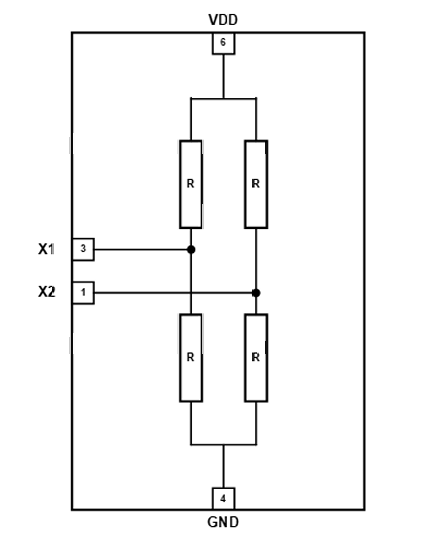
\includegraphics[height=6.5cm, keepaspectratio]{ct100-wheatstone.pdf.png}
    \\[3mm]
    \small (a) CT100 internal Wheatstone-bridge.
  \end{minipage}% <-- % prevents line break between minipages
  \hfill
  % --- RIGHT SIDE: Matched Circuit Schematic ---
  \begin{minipage}[b]{0.52\textwidth}
    \centering
    \begin{circuitikz}[american voltages, european resistors, scale=0.85, transform shape]
      
      % American DC Voltage Source (VDD) - 6 units tall
      \draw (0,0) to[american voltage source, invert, l=$V_{\text{DD}}$] (0,6)
            -- (2,6);
      \draw (0,0) -- (2,0);

      % Top & Bottom Rails with Connection Dots
      \draw (2,6) to[short, *-] (4,6);
      \draw (2,0) to[short, *-] (4,0);
      \draw (2,0) node[sground] {};

      % Left Bridge Leg (R1: 5.2 to 3.6, R3: 2.4 to 0.8)
      \draw (2,6) -- (2,5.2)
            to[R=$R_1$] (2,3.6)
            -- (2,2.4)
            to[R=$R_3$] (2,0.8)
            -- (2,0);

      % Right Bridge Leg (R2: 5.2 to 3.6, R4: 2.4 to 0.8)
      \draw (4,6) -- (4,5.2)
            to[R=$R_2$] (4,3.6)
            -- (4,2.4)
            to[R=$R_4$] (4,0.8)
            -- (4,0);

      % Output Line X1 (Tapped from left leg at y=3.2 with junction dot directly on x=2)
      \draw (2,3.2) to[short, *-o] (5.5,3.2) node[right] {$X_1$};

      % Output Line X2 (Tapped from right leg at y=2.8 with junction dot directly on x=4)
      \draw (4,2.8) to[short, *-o] (5.5,2.8) node[right] {$X_2$};

    \end{circuitikz}
    \\[3mm]
    \small (b) Equivalent bridge schematic.
  \end{minipage}

  \caption{Internal CT100 IC pin configuration alongside its labeled equivalent electrical schematic.}
  \label{fig:wheatstone_comparison}
\end{figure}


% 2. MATHEMATICAL DERIVATION SECOND
To predict the maximum differential output voltage prior to saturation, the CT100's internal TMR Wheatstone bridge (Figure~\ref{fig:wheatstone_comparison}a) was evaluated theoretically. An equivalent schematic with explicitly labeled internal elements is provided in Figure~\ref{fig:wheatstone_comparison}b to aid in following the derivation below.  According to the device datasheet \cite{ct100_datasheet}, the per-element resistance ranges from $R_{\min} \approx \SI{20}{\kilo\ohm}$ (parallel magnetic alignment, lowest-resistance state) to $R_{\max} \approx \SI{40}{\kilo\ohm}$ (antiparallel magnetic alignment, highest-resistance state). 

As a result of this Wheatstone-bridge configuration, the largest change in $\left|V_{\text{out}} \right|$ is $\frac{V_{\text{DD}}}{3}$:
\begin{equation}
   \left| \Delta V_{\text{out,max}} \right| = \frac{V_{\text{DD}}}{3}
\end{equation}
The maximum output swing is bounded by the resistance range of each element, from $R_{\min} \approx \SI{20}{\kilo\ohm}$ to $R_{\max} \approx \SI{40}{\kilo\ohm}$.

The voltage potentials at the two central output nodes, $X_1$ and $X_2$, as seen in Figure~\ref{fig:wheatstone_comparison}b are determined by the independent voltage divider ratios along the bridge:
\begin{equation}
    X_1 = V_{\text{DD}} \cdot \left( \frac{R_3}{R_1 + R_3} \right), \qquad X_2 = V_{\text{DD}} \cdot \left( \frac{R_4}{R_2 + R_4} \right)
    \label{eq:node_voltages}
\end{equation}

The general differential output voltage $V_{\text{out}}$ across nodes $X_1$ and $X_2$ is expressed as:
\begin{equation}
    V_{\text{out}} = X_1 - X_2 = V_{\text{DD}} \left( \frac{R_3}{R_1 + R_3} - \frac{R_4}{R_2 + R_4} \right)
    \label{eq:vout_general}
\end{equation}

At $B = \SI{0}{\tesla}$, all four TMR elements exhibit nominal, equal resistance ($R_1 = R_2 = R_3 = R_4$), yielding balanced potentials $X_1 = X_2 = \frac{V_{\text{DD}}}{2}$ and $V_{\text{out}} = \SI{0}{\volt}$. 

A key operational characteristic of the CT100 is that an external magnetic field applied along its sensitive axis drives opposing element pairs in opposite resistance directions. As one pair (\(R_1, R_4\)) decreases toward \(R_{\min}\), the complementary pair (\(R_2, R_3\)) increases toward \(R_{\max}\) or vice versa. This response is governed by the orientation of the pinned ferromagnetic reference layer within each TMR element: \(R_1\) and \(R_4\) share an identical reference layer alignment, whereas \(R_2\) and \(R_3\) are pinned in the opposite direction.

 At full magnetic saturation, the opposing resistor pairs settle at either $R_{\min}$ and $R_{\max}$. For this derivation, an external magnetic field polarity is assumed such that:

\begin{equation}
R_1 = R_4 = R_{\min}, \quad \text{and} \quad R_2 = R_3 = R_{\max}
\label{eq:tmr-saturation-resistances}
\end{equation}

Substituting these saturation values into Equation~\ref{eq:node_voltages} gives the node potentials at full saturation:
\begin{equation}
    X_{1,\text{sat}} = V_{\text{DD}} \cdot \left( \frac{R_{\max}}{R_{\min} + R_{\max}} \right), \qquad X_{2,\text{sat}} = V_{\text{DD}} \cdot \left( \frac{R_{\min}}{R_{\max} + R_{\min}} \right)
\end{equation}

Subtracting $X_{2,\text{sat}}$ from $X_{1,\text{sat}}$ yields the maximum theoretical differential output voltage $V_{\text{out,sat}}$:
\begin{equation}
    V_{\text{out,sat}} = X_{1,\text{sat}} - X_{2,\text{sat}} = V_{\text{DD}} \left( \frac{R_{\max} - R_{\min}}{R_{\max} + R_{\min}} \right)
    \label{eq:vout_sat_derived}
\end{equation}

Substituting the CT100 datasheet resistance values \cite{ct100_datasheet} ($R_{\min} = \SI{20}{\kilo\ohm}$ and $R_{\max} = \SI{40}{\kilo\ohm}$):
\begin{equation}
    V_{\text{out,sat}} = V_{\text{DD}} \left( \frac{\SI{40}{\kilo\ohm} - \SI{20}{\kilo\ohm}}{\SI{40}{\kilo\ohm} + \SI{20}{\kilo\ohm}} \right) = V_{\text{DD}} \left( \frac{20}{60} \right) = \frac{V_{\text{DD}}}{3}
\end{equation}

The output is therefore bounded to $\left| V_{\text{out}} \right| \le V_{\text{DD}}/3$. For $V_{\text{DD}} = \SI{3.30}{\volt}$ the ceiling is $\SI{1.10}{\volt}$; this is tested in Section~\ref{sec:standalone-sat-recovery}.

The direction of the applied field along the sensitive axis decides which resistor pair moves to $R_{\min}$, so the bridge can saturate at either polarity. The two limits, $V_{\text{out}} = +V_{\text{DD}}/3$ and $V_{\text{out}} = -V_{\text{DD}}/3$, are called the \textbf{positive ceiling} and the \textbf{negative ceiling} respectively. The negative ceiling follows from the derivation above by swapping $R_{\min}$ and $R_{\max}$. In this report, \emph{ceiling} means the saturation limit of $V_{\text{out}}$, and its sign states which of the two was reached.

% 3. DEFINITION STATEMENT THIRD
From here on, the sensor output is defined as $V_{\text{out}} = X_1 - X_2$ for every instrument used (DMM, oscilloscope and MCU).



\section{Available Instrumentation}
\label{sec:instrumentation}

Characterization and bench-top tests were conducted using the following laboratory equipment to ensure power delivery and take measurements.

\begin{itemize}
    \item \textbf{Digital Oscilloscope:} Rohde \& Schwarz RTB2002 (\SI{2.5}{GS/s} sampling rate, 10-bit A/D converter) for transient analysis, step-response monitoring across nodes \(X_1\) and \(X_2\).
    \item \textbf{ Digital Multimeter (DMM):} Keithley 2110 \(5\frac{1}{2}\) Digit Dual-Display Multimeter for DC Voltage and Current logging and cross-validating MCU reading accuracy.
    
    \item \textbf{DC Power Supply Unit (PSU):} Topward dual-tracking linear DC power supply capable of supplying up to \SI{6.0}{\ampere} continuously, providing supply voltage  and current excitation through the PCB test trace.
    
    \end{itemize}

\section{Standalone Sensor Board}
\label{sec:standalone-board}

Before adding any electronics, the bare sensor was characterised on its own. This gives a reference for how the CT100 itself behaves, so that any later change in behaviour can be attributed to the circuit, to radiation or to saturation rather than to the sensor. The results answer H1 (the saturation ceiling) and give the first measurement for H3 (recovery time).

\subsection{PCB Design}
\label{sec:standalone-pcb}

To measure the CT100's saturation limits and test the derivation in Section~\ref{sec:bridge-topology}, a standalone board was designed in Altium Designer and populated with only the CT100 and a \SI{0.1}{\micro\farad} decoupling capacitor.

The board is powered from a laboratory PSU, and the outputs $X_1$ and $X_2$ are measured with the oscilloscope and the DMM. No amplifier was included, because an amplifier's slew rate and bandwidth could slow the measured recovery and hide the response of the bridge itself. Measuring the unconditioned bridge therefore gives a baseline for the sensor's own saturation and recovery. The same board was used by Daniel Tieu for thermal cycling, and it is shown in Figure~\ref{fig:standalone}.

\begin{figure}[H]
\centering
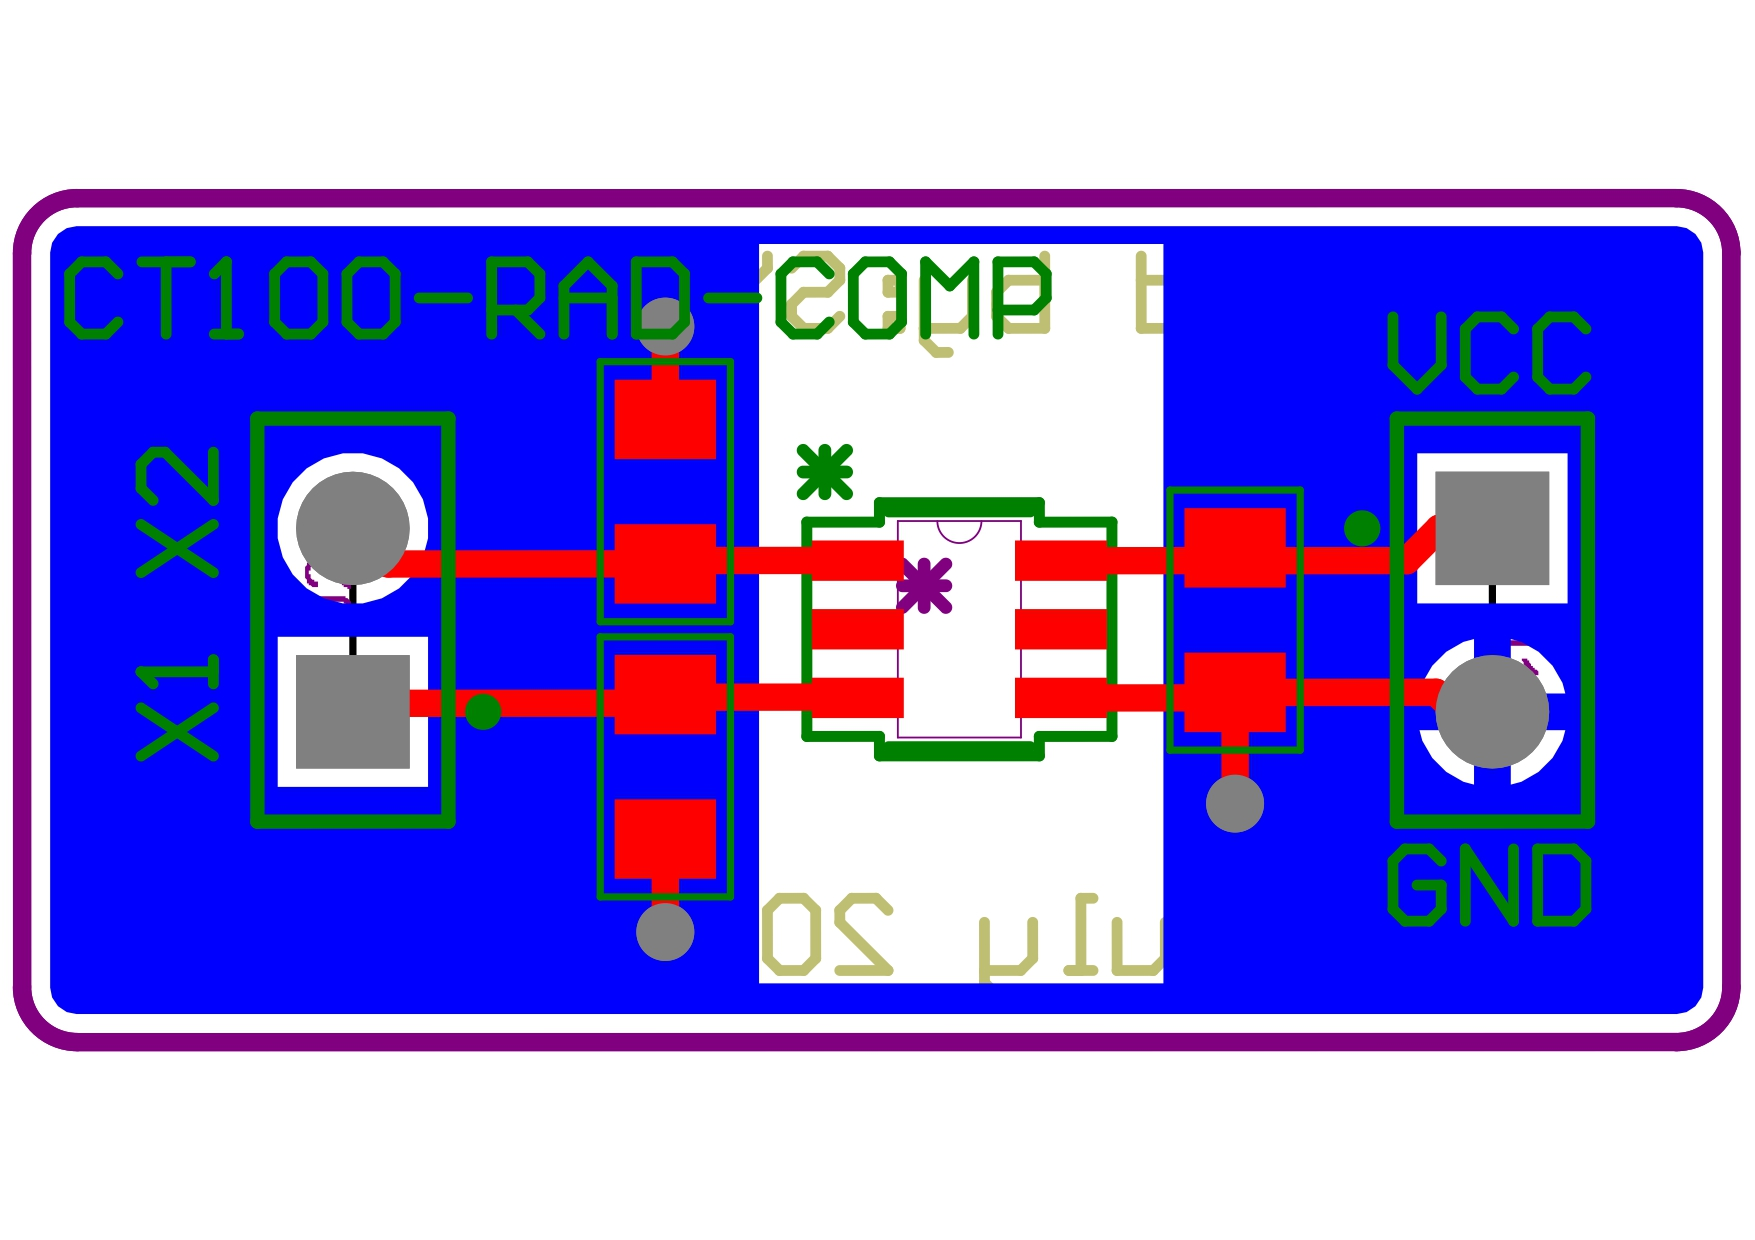
\includegraphics[width=0.7\textwidth]{TMR_RAD_COMPARE_page-0001.jpg}
\caption{Standalone Sensor PCB}
\label{fig:standalone}
\end{figure}


\subsection{Saturation Testing Methodology}


\label{sec:sat-test-methodology}


Saturation was induced with a hand-held LM-1618 neodymium magnet, the simplest stimulus available for a first characterisation, although it is neither repeatable nor automatable. The aim was to drive the sensor well beyond its $\pm\SI{50}{\milli\tesla}$ operating range, to characterise recovery after the worst case, while staying near or below its $\pm\SI{200}{\milli\tesla}$ absolute-maximum rating, above which reliability may be affected \cite{ct100_datasheet}.

The magnet used was an LM-1618 neodymium disc, \SI{25}{\milli\metre} in diameter and \SI{5}{\milli\metre} thick, with a remanence $B_r$ of 1180 to \SI{1220}{\milli\tesla} \cite{lm1618_datasheet}. The remanence is a property of the material, not the field outside the magnet. On the axis of a disc magnet of radius $R$ and thickness $L$, treating the magnet as an ideal solenoid \cite{camacho2013,shulman2022}, the field at distance $z$ from its face is
\begin{equation}
B(z) = \frac{B_r}{2}\left[\frac{L+z}{\sqrt{R^2+(L+z)^2}} - \frac{z}{\sqrt{R^2+z^2}}\right],
\label{eq:disc-magnet}
\end{equation}
which gives about \SI{223}{\milli\tesla} at the face, \SI{152}{\milli\tesla} at \SI{5}{\milli\metre} and \SI{86}{\milli\tesla} at \SI{10}{\milli\metre}. Within about a centimetre the field is therefore well beyond the CT100's $\pm\SI{50}{\milli\tesla}$ operating range, which guarantees saturation, while staying close to or below its \SI{200}{\milli\tesla} absolute-maximum rating \cite{ct100_datasheet}, since the package itself keeps the sensing element away from the magnet face.

During each test the oscilloscope confirmed that the output had reached the ceiling of about $V_{\text{DD}}/3$ derived in Section~\ref{sec:bridge-topology}. The magnet was then removed quickly, and the oscilloscope captured the output as it fell back to its zero-field baseline.

Every saturation result in this report is presented in the same table format, with the same definitions:
\begin{itemize}
\item \textbf{Sample:} the unit tested. Samples 1 to 4 are sensor-only boards (1 and 2 non-irradiated, 3 and 4 irradiated). Boards A, B and C are integrated boards (A non-irradiated, B irradiated, C a fresh sensor used for the hysteresis test in Section~\ref{sec:hysteresis}).
\item \textbf{Ceiling (V):} the output voltage $V_{\text{out}}$ reached at saturation. Its sign shows which ceiling was reached, so each sample has one row per ceiling.
\item \textbf{Baseline (mV):} the output once it has settled after the field is removed.
\item \textbf{Swing (V):} the size of the drop from the ceiling to the baseline, $|{\rm ceiling} - {\rm baseline}|$.
\item \textbf{Recovery (ms):} the time from the start of the fall until the output has settled at its baseline. On the oscilloscope this is read with cursors; for the MCU (SWV) traces it is the time until the output stays within $\SI{5}{\milli\volt}$ of its final baseline. Five millivolts is also about the oscilloscope's vertical resolution at $\SI{500}{\milli\volt}$/div, so the two definitions of ``settled'' are comparable.
\end{itemize}


\subsection{Sensor-Only Saturation and Recovery Behaviour}
\label{sec:standalone-sat-recovery}

Two non-irradiated sensor-only samples (Samples 1 and 2) were each driven to both ceilings. Testing both directions checks a prediction of the bridge model: the ceilings should be symmetric about zero, $\pm V_{\text{DD}}/3$ (Section~\ref{sec:bridge-topology}), because the same spin-tunnelling limit applies to either polarity. The extracted values are listed in Table~\ref{tab:sat-nonirr-sensoronly}, and the oscilloscope captures they come from are shown in Figure~\ref{fig:scope-baseline}.

The CT100 is sensitive to the field component along one in-plane axis of its package. The datasheet defines a positive field as one directed into the pin~1/pin~6 side of the package, which makes $X_1 > X_2$ \cite{ct100_datasheet}. Which ceiling is reached therefore depends only on which pole of the magnet faces that side of the package: one pole drives $V_{\text{out}}$ to the positive ceiling and the opposite pole to the negative ceiling.


\begin{table}[H]
\centering
\caption{Saturation recovery results, non-irradiated sensor-only samples.}
\label{tab:sat-nonirr-sensoronly}
\begin{tabular}{@{}lrrrr@{}}
\toprule
Sample & Ceiling (V) & Baseline (mV) & Swing (V) & Recovery (ms) \\
\midrule
1 & $-1.126$ & $-17.4$ & 1.108 & 76.5 \\
1 & $+1.125$ & $-12.5$ & 1.138 & 74.0 \\
2 & $-1.145$ & $-17.4$ & 1.128 & 76.0 \\
2 & $+1.125$ & $-12.5$ & 1.138 & 67.5 \\
\bottomrule
\end{tabular}
\end{table}


Figure~\ref{fig:scope-baseline} shows the oscilloscope captures for Samples 1 and 2 at both ceilings. The blue trace ($M_1$) is the differential output $V_{\text{out}} = X_1 - X_2$, and the yellow ($C_1$) and green ($C_2$) traces are the bridge outputs $X_1$ and $X_2$.

\begin{figure}[H]
    \centering
    % Top Row: Sample 1
    \begin{subfigure}[b]{0.48\textwidth}
        \centering
        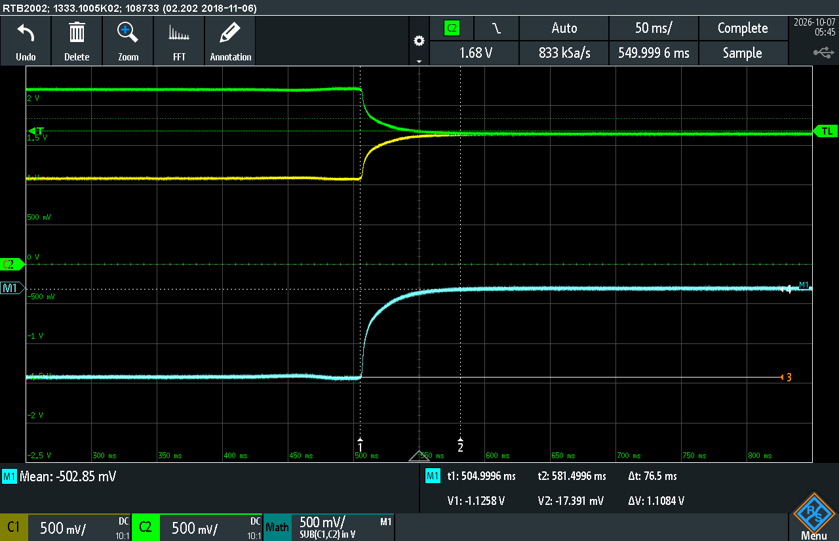
\includegraphics[width=\textwidth]{1_satn.png}
        \caption{Sample 1: Negative Saturation Recovery}
        \label{fig:1_satn}
    \end{subfigure}
    \hfill
    \begin{subfigure}[b]{0.48\textwidth}
        \centering
        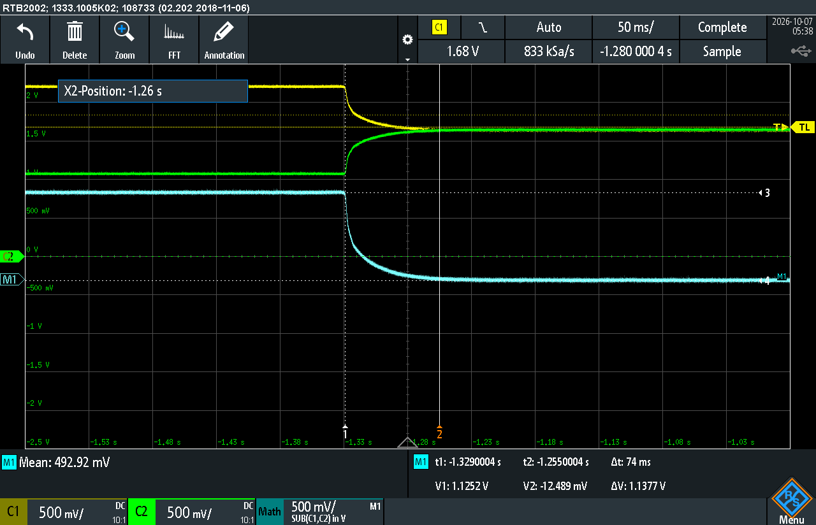
\includegraphics[width=\textwidth]{1_satp.png} % Assuming this filename based on your convention
        \caption{Sample 1: Positive Saturation Recovery}
        \label{fig:1_satp}
    \end{subfigure}
    
    \vspace{0.5cm} % Vertical spacing between rows
    
    % Bottom Row: Sample 2
    \begin{subfigure}[b]{0.48\textwidth}
        \centering
        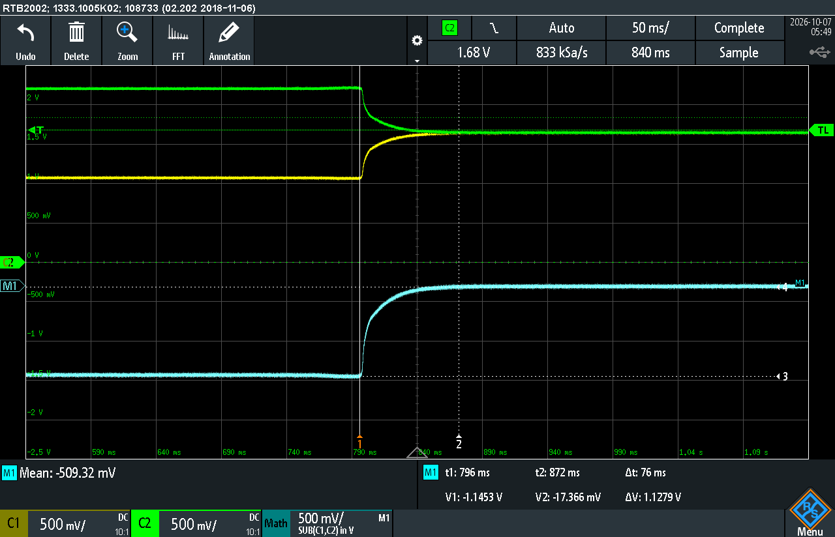
\includegraphics[width=\textwidth]{2_satn.png}
        \caption{Sample 2: Negative Saturation Recovery}
        \label{fig:2_satn}
    \end{subfigure}
    \hfill
    \begin{subfigure}[b]{0.48\textwidth}
        \centering
        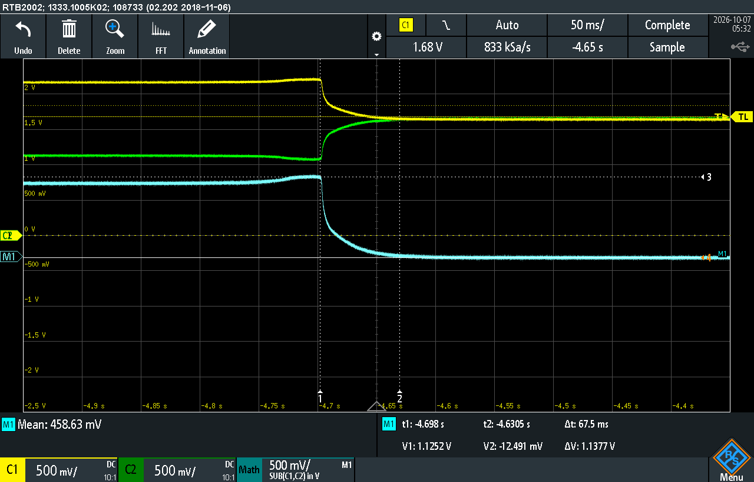
\includegraphics[width=\textwidth]{2_satp.png}
        \caption{Sample 2: Positive Saturation Recovery}
        \label{fig:2_satp}
    \end{subfigure}
    
    \caption{Oscilloscope traces capturing the saturation ceiling and subsequent transient recovery for the non-irradiated sensors.}
    \label{fig:scope-baseline}
\end{figure}
Across the four captures the mean recovery time is $\SI{73.5}{\milli\second}$, with a maximum of $\SI{76.5}{\milli\second}$. Because the magnet was withdrawn by hand, these times include the effect of the withdrawal speed. What they mean for a CubeSat magnetometer, including the guard window that flight software would need after a saturating event, is assessed in Section~\ref{sec:disc-recovery} once all samples have been presented.



\section{Integrated Board: Field Excitation and Design}
\label{sec:integrated-board}

A hand-held magnet cannot produce a known field, so it cannot measure sensitivity, and it cannot be automated. The integrated board solves both problems: a current-carrying trace produces a field that can be calculated from the measured current, and the microcontroller logs the sensor output without an operator. This board is the low-cost, reusable test method named in the aims, and it is used for every test of sensitivity (H2), lasting change (H4), radiation (H5) and shielding (H6).

\subsection{Integrated Board Design}
\label{sec:integrated-design}

Measuring sensitivity needs a repeatable test field of known size. It is produced by a current-carrying trace routed directly beneath the sensor. The field of the trace is calculated analytically (Section~\ref{sec:field-model}) and simulated in Ansys Maxwell (Section~\ref{sec:field-validation}), giving a theoretical benchmark for the measured output. The PSU's \SI{6.0}{\ampere} limit gives a field of only about \SI{0.5}{\milli\tesla}, far too small to saturate the sensor, but enough for a linear sweep from which the sensitivity is found. This sweep is the baseline against which any change caused by saturation or radiation is later measured.

The integrated board is built around three components:

\begin{itemize}
    \item \textbf{Microcontroller (MCU):} An STM32G431KBT6 \cite{stm32g4_rm} reads the CT100's outputs directly on a differential ADC channel, at \SI{1.0}{\kilo\hertz} with 12-bit resolution. The ADC's built-in calibration runs at start-up to reduce differences between boards.
    
    \item \textbf{Current Monitor (INA219)~\cite{ina219_datasheet}:} Because the PSU's analogue display was not precise enough, the trace current is measured by an INA219 across a Kelvin-connected \SI{5.0}{\milli\ohm} shunt. The measured current is used to calculate the field applied to the sensor.
    
    \item \textbf{Low-Dropout (LDO) regulator:} A \SI{5.0}{\volt} input is regulated to \SI{3.30}{\volt}, which supplies both the sensor and the MCU. The regulator's power-supply rejection keeps supply noise out of the bridge, and because the same rail is the ADC's reference, its value sets the size of one ADC step.
    
\end{itemize}


As Figure~\ref{fig:board} shows, the current-carrying trace (blue polygon) runs on the bottom layer, in series with a 2512 shunt resistor. Figure~\ref{fig:excitation_circuit} defines the positive current direction ($+i$) used for all field calculations and sweeps. The full Altium schematic is in Appendix~A.

\begin{figure}[H]
\centering
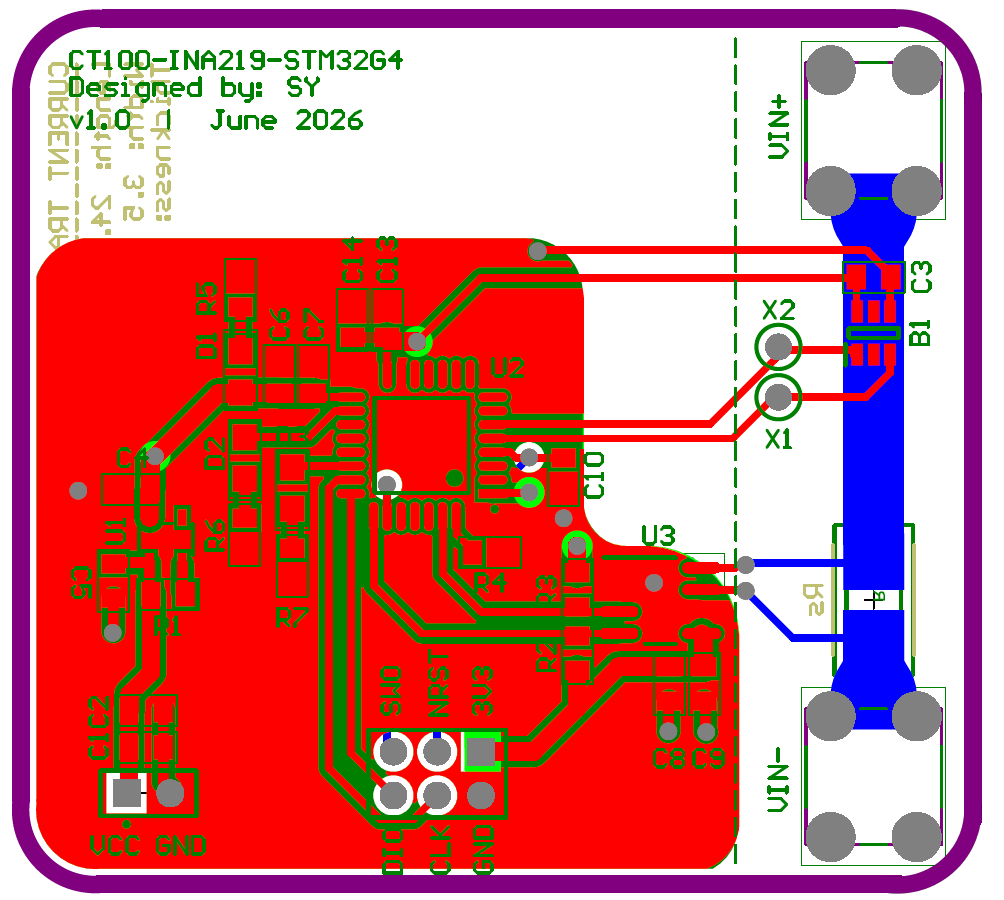
\includegraphics[width=0.47\textwidth]{magsat_layout.png}\hfill
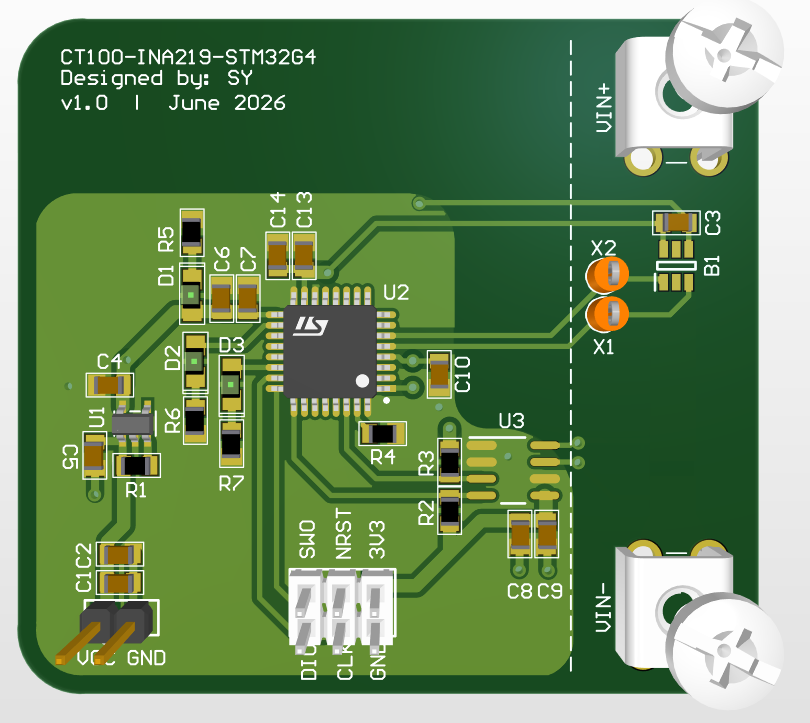
\includegraphics[width=0.47\textwidth]{magsat_pcb_front.png}
\caption{Integrated board layout (left) and rendered assembly view (right).}
\label{fig:board}
\end{figure}

\begin{figure}[htbp]
\centering

\begin{circuitikz}[scale=1.1, transform shape]
    % Terminals on the right using standard path poles (-o)
    \draw (3,3) to[short, -o] (5,3) node[right] {\textbf{\(V_{\text{IN}}^+\)}};
    \draw (3,0) to[short, -o] (5,0) node[right] {\textbf{\(V_{\text{IN}}^-\)}};

    % Top horizontal rail with leftward positive current arrow (+i)
    \draw (3,3) to[short, i_=\(+i\)] (0,3);

    % Bottom horizontal rail
    \draw (0,0) -- (3,0);

    % Middle vertical branch: Upward Current Source (i)
    \draw (3,0) to[american current source, l_=\(i\)] (3,3);

    % Junction nodes at the T-connections (filled dots)
    \node[circ] at (3,3) {};
    \node[circ] at (3,0) {};

    % Far-left branch: European Resistor R_shunt
    \draw (0,3) to[R, european, l_=\(R_{\text{shunt}}\)] (0,0);

\end{circuitikz}
\caption{Field excitation circuit schematic and positive trace current convention (\(+i\)).}
\label{fig:excitation_circuit}
\label{fig:excitation_schematic_v2}
\end{figure}

Figure~\ref{fig:excitation_circuit} models the excitation as an ideal current source $i$; in practice a bench PSU in constant-current mode sets the current through $R_{\text{shunt}}$ and the trace.

\subsection{PCB Trace Design}
\label{sec:pcb-trace}

The current-carrying trace is routed on a four-layer PCB whose stack-up is given in Table~\ref{tab:stackup}, so that its field lies along the sensor's sensing axis.

No copper pour was placed on any layer directly beneath the sensor, so that no plane or return currents flow close to the sensing element and the only board-generated field at the die is that of the excitation trace. Copper is non-magnetic, so the concern is current flowing in nearby copper rather than the copper itself distorting a static field.

\begin{table}[H]
\centering
\caption{Four-layer PCB stack-up, from the Altium Layer Stack Manager.}
\label{tab:stackup}
\begin{tabular}{@{}lllrr@{}}
\toprule
Layer & Material & Type & Thickness (mm) & $D_k$ \\
\midrule
Top solder mask & SM-001 & Solder mask & 0.0254 & 4.0 \\
Top layer & CF-004, 1\,oz & Signal & 0.0350 & --- \\
Dielectric 4 & PP-017 & Prepreg & 0.1295 & 4.3 \\
Dielectric 2 & PP-017 & Prepreg & 0.1295 & 4.3 \\
Layer 2 (GND) & CF-001, 1/4\,oz & Signal & 0.0090 & --- \\
Dielectric 1 & FR-4 & Core & 0.3200 & 4.8 \\
Layer 3 (PWR) & CF-001, 1/4\,oz & Signal & 0.0090 & --- \\
Dielectric 3 & PP-017 & Prepreg & 0.1295 & 4.3 \\
Dielectric 5 & PP-017 & Prepreg & 0.1295 & 4.3 \\
Bottom layer (trace) & CF-004, 1\,oz & Signal & 0.0350 & --- \\
Bottom solder mask & SM-001 & Solder mask & 0.0254 & 4.0 \\
\midrule
Total & & & 0.9770 & \\
\bottomrule
\end{tabular}
\end{table}
 
The board is $\SI{0.977}{\milli\metre}$ thick in total: $\SI{0.088}{\milli\metre}$ of copper and $\SI{0.838}{\milli\metre}$ of dielectric, made up of four $\SI{0.130}{\milli\metre}$ prepreg layers and a $\SI{0.320}{\milli\metre}$ FR-4 core. The excitation trace is on the bottom layer, with a width $w = \SI{3.5}{\milli\metre}$, sized to carry the PSU's $\SI{6.0}{\ampere}$ limit.

\subsection{Analytical Field Model}
\label{sec:field-model}

The horizontal magnetic field at the sensing element, a height $d$ above the centre of the trace of width $w = \SI{3.5}{\milli\metre}$, is modelled as the field of a thin flat strip conductor:
\begin{equation}
B_{\text{planar}} = \mu_0 \left[ \frac{I}{\pi w} \arctan\left( \frac{w}{2d} \right) \right].
\label{eq:planar}
\end{equation}

The trace is treated as a thin flat strip of width $w$ carrying the current $I$ uniformly, so it can be split into long straight filaments of width $\mathrm{d}x$, each carrying $\mathrm{d}I = (I/w)\,\mathrm{d}x$. A long straight filament produces a field $\mu_0\,\mathrm{d}I/(2\pi r)$ at distance $r$ \cite{openstax_up2}. At a height $d$ above the centre of the strip, the vertical components from filaments on either side cancel by symmetry, and the horizontal components add, so
\begin{equation}
B = \int_{-w/2}^{w/2} \frac{\mu_0 I}{2\pi w}\,\frac{d}{x^2+d^2}\,\mathrm{d}x = \frac{\mu_0 I}{\pi w}\arctan\!\left(\frac{w}{2d}\right),
\end{equation}
which is Equation~\eqref{eq:planar}.

The distance $d$ is measured from the mid-plane of the bottom-layer trace to the sensing element. From Table~\ref{tab:stackup}, that mid-plane lies $\SI{0.909}{\milli\metre}$ below the top copper surface: half of the $\SI{0.035}{\milli\metre}$ trace, the $\SI{0.838}{\milli\metre}$ of dielectric, the two $\SI{0.009}{\milli\metre}$ inner copper layers and the $\SI{0.035}{\milli\metre}$ top copper. The datasheet places the sensing element $0.76 \pm \SI{0.087}{\milli\metre}$ above the bottom of the SOT23-6 package body, and the body stands a typical $\SI{0.10}{\milli\metre}$ (0 to $\SI{0.15}{\milli\metre}$) above the board \cite{ct100_datasheet}. The sensing element is therefore $h_s \approx \SI{0.86}{\milli\metre}$ above the top copper, and
\begin{equation}
d = \SI{0.909}{\milli\metre} + h_s \approx \SI{1.77}{\milli\metre}.
\label{eq:d-stackup}
\end{equation}
The solder joint under the leads adds a few tens of micrometres and is neglected. Taking the tolerances on the sensor position and the package stand-off together, $d$ lies between 1.58 and $\SI{1.91}{\milli\metre}$.

Normalizing Equation~\eqref{eq:planar} by the trace current $I$ yields the geometric field coupling coefficient $k_B$:
\begin{equation}
k_B = \frac{B_{\text{planar}}}{I} = \frac{\mu_0}{\pi w} \arctan\left( \frac{w}{2d} \right) \approx \SI{0.0892}{\milli\tesla\per\ampere},
\label{eq:field-coeff}
\end{equation}

with a range of 0.085 to $\SI{0.096}{\milli\tesla\per\ampere}$ over the tolerance on $d$. At a representative excitation current of $I = \SI{4.175}{\ampere}$ this gives a field of $\SI{372}{\micro\tesla}$. Combining $k_B$ with the CT100 sensor's sensitivity $S_V$ (\si{\milli\volt\per\milli\tesla}) gives the expected differential voltage change per unit trace current:
\begin{equation}
\frac{\Delta V_{\text{out}}}{\Delta I} = k_B \cdot S_V.
\label{eq:sensitivity-transfer}
\end{equation}

This analytical transfer ratio serves as the theoretical benchmark against which both the Ansys Maxwell finite-element simulations and empirical linear current sweeps are validated.

\subsection{Simulated vs.\ Experimental Field Validation}
\label{sec:field-validation}

The analytical field model was cross-checked against a finite-element simulation in Ansys Maxwell (Figure~\ref{fig:ansys}), which resolves the full 3D field around the trace rather than the infinite 2D strip assumed by Equation~\eqref{eq:planar}. The simulation gave about $\SI{500}{\micro\tesla}$ at $\SI{4.175}{\ampere}$ on its evaluation plane. In the analytical model this field occurs at a height of about $\SI{1.0}{\milli\metre}$, closer to the trace than the datasheet sensor position of $\SI{1.77}{\milli\metre}$, which indicates that the simulation evaluated the field on a plane closer to the trace than the sensing element; at the same height the two models agree. \todo{Re-run the Ansys model with the field evaluated at $d = \SI{1.77}{\milli\metre}$, the datasheet sensor height, and update this paragraph and Figure~\ref{fig:ansys}. The analytical model predicts \SI{372}{\micro\tesla} there.}

The measured output at $\SI{4.175}{\ampere}$ (about $\SI{16}{\milli\volt}$ on the DMM) cannot be compared directly with the model, because it includes the sensor's zero-field offset of about $\SI{13}{\milli\volt}$ on this board. The like-for-like comparison is the gradient of output against current, which a fixed offset does not affect. It is made in Section~\ref{sec:sensitivity-fit}, where the measured gradient agrees with the model to within a few percent.



\begin{figure}[h]
\centering
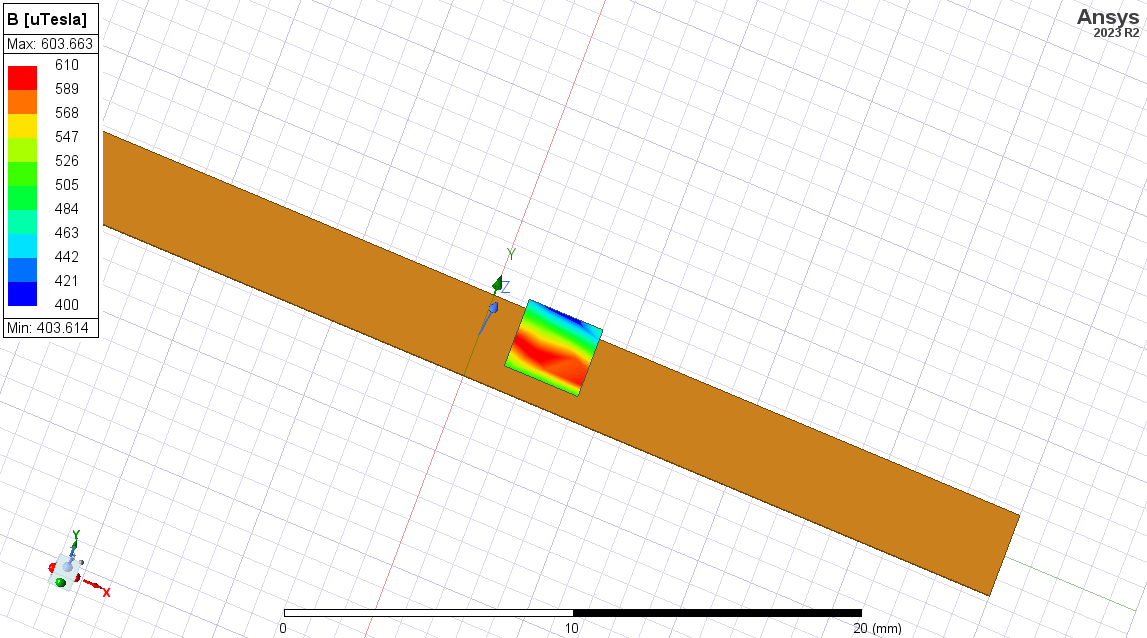
\includegraphics[width=0.75\textwidth]{anys_trace.png}
\caption{Ansys near-field simulation of the current trace.}
\label{fig:ansys}
\end{figure}



\subsection{Firmware}
\label{sec:firmware}

The firmware is built upon the STM32 Hardware Abstraction Layer (HAL). The MCU's ADC is configured in differential-pair mode, sampling \(X_1 - X_2\) directly and converting the raw 12-bit value to volts via:
\begin{equation}
X_1 - X_2 = \left( \frac{\text{ADC}_{\text{raw}} - 2048}{2048} \right) \times V_{\text{DD}}
\label{eq:adcconv}
\end{equation}
where 2048 is the mid-scale ADC code corresponding to the zero-differential (balanced-bridge) midpoint. Hardware ADC self-calibration (\texttt{HAL\_ADCEx\_Calibration\_Start}) is executed automatically on every boot before any conversions occur. The MCU continuously polls the INA219 over \(\text{I}^2\text{C}\) for trace current and streams both the current and voltage values out in real time over the Serial Wire Viewer (SWV) debug channel for offline analysis in MATLAB. 


\subsection{Design Note for Future PCB Revisions}
\label{sec:future-pcb-note}

Because the sensor bridge is nominally balanced at \(V_{\text{DD}}/2\) as noted in Section~\ref{sec:bridge-topology}, the ADC channel monitoring it spends its full dynamic range on either side of that midpoint. Any measurement taken near the zero-differential code inherits the ADC's own quantization and calibration uncertainty around that center point.

A future revision of the integrated board could add a small reference offset at the ADC input, so that zero field no longer sits exactly on the mid-scale code. This should reduce the error from operating at the ADC's most quantisation-sensitive point; it was not implemented or tested in this project.




\section{Non-Irradiated Sensitivity and Saturation Characterisation}
\label{sec:nonirr-characterisation}

\subsection{Linear Fitting and the Coefficient of Determination}
\label{sec:fitting}
 
Every current sweep in this report is summarised by a straight line,
\begin{equation}
V_{\text{out}} = m I + c,
\label{eq:linfit}
\end{equation}
where $m$ is the gradient in $\si{\milli\volt\per\ampere}$ and $c$ is the offset, the output at zero trace current. The line is fitted by ordinary least squares, which chooses $m$ and $c$ to minimise the sum of the squared differences between the measured outputs $V_i$ and the fitted values $\hat{V}_i = m I_i + c$.
 
How well the line describes the data is given by the coefficient of determination,
\begin{equation}
R^2 = 1 - \frac{\sum_i (V_i - \hat{V}_i)^2}{\sum_i (V_i - \bar{V})^2},
\label{eq:r2}
\end{equation}
where $\bar{V}$ is the mean of the measured outputs. The numerator is the scatter left over after the fit and the denominator is the total spread of the data, so $R^2$ is the fraction of the variation in the output that the straight line explains. A value of 1 means every point lies exactly on the line; a value of 0 means the line explains none of the variation. In this report $R^2$ is used only as a measure of linearity. A high $R^2$ shows that the output is proportional to current over the sweep, but it does not show that the gradient is correct; that is checked separately against the theoretical gradient. $R^2$ is also unaffected by a constant offset, so a sweep with a large zero-field offset can still have $R^2$ close to 1.
 
The uncertainty of each gradient is given by its standard error,
\begin{equation}
s_m = \sqrt{\frac{\sum_i (V_i - \hat{V}_i)^2 / (n-2)}{\sum_i (I_i - \bar{I})^2}},
\label{eq:slope-se}
\end{equation}
where $n$ is the number of points in the sweep (13 for every sweep here). Gradients are reported as $m \pm s_m$. Two gradients are treated as different only if they differ by clearly more than their combined standard error, $\sqrt{s_{m,1}^2 + s_{m,2}^2}$.

\subsection{Saturation Recovery on the Integrated Board}
\label{sec:sat-recovery-integrated}

This subsection repeats the saturation test on the integrated board, with the output logged by the MCU instead of the oscilloscope, so that the two hardware configurations can be compared. The board was run from a regulator input of $V_{\text{CC}} = \SI{4.97}{\volt}$, giving a sensor supply of $V_{\text{DD}} = \SI{3.32}{\volt}$.

\begin{table}[H]
\centering
\caption{Saturation recovery results, non-irradiated integrated board (Board A).}
\label{tab:sat-ceiling-intl}
\begin{tabular}{@{}lrrrr@{}}
\toprule
Sample & Ceiling (V) & Baseline (mV) & Swing (V) & Recovery (ms) \\
\midrule
A & $-1.152$ & $-8.1$ & 1.144 & 65.2 \\
A & $+1.138$ & $+12.9$ & 1.125 & 60.2 \\
\bottomrule
\end{tabular}
\end{table}



\begin{figure}[H]
\centering
\begin{tikzpicture}
\begin{groupplot}[
    group style={group size=2 by 2, horizontal sep=1.5cm, vertical sep=1.7cm},
    width=0.48\textwidth, height=0.36\textwidth,
    xmin=-20, xmax=150, grid=major, grid style={gray!25}, axis lines=box,
    tick label style={font=\footnotesize}, label style={font=\small}, title style={font=\small},
]
\nextgroupplot[title={(a) Non-irradiated, negative saturation recovery }, ylabel={$V_{\text{out}}$ (V)}, ymin=-1.3, ymax=0.2, xlabel={Time since rising edge (ms)}]
\addplot[blue!70!black, thick] table[col sep=comma, x=t_ms, y=v_V] {rec_nonirr_neg.csv};
\draw[dashed] (axis cs:65.2,-1.3) -- (axis cs:65.2,0.2);
\node[font=\scriptsize, anchor=north west, fill=white, inner sep=1pt] at (axis cs:68,-0.55) {$t_{\text{rec}}=65.2$ ms};
\node[font=\scriptsize, anchor=west] at (axis cs:5,-1.1) {ceiling $-1.152$ V};

\nextgroupplot[title={(b) Non-irradiated, positive saturation recovery }, ymin=-0.2, ymax=1.3, xlabel={Time since falling edge (ms)}]
\addplot[blue!70!black, thick] table[col sep=comma, x=t_ms, y=v_V] {rec_nonirr_pos.csv};
\draw[dashed] (axis cs:60.2,-0.2) -- (axis cs:60.2,1.3);
\node[font=\scriptsize, anchor=south west, fill=white, inner sep=1pt] at (axis cs:63,0.45) {$t_{\text{rec}}=60.2$ ms};
\node[font=\scriptsize, anchor=west] at (axis cs:2,1.1) {ceiling $+1.138$ V};

\end{groupplot}
\end{tikzpicture}
\caption{Non-Irradiated Saturation recovery on the integrated board after the magnet is removed, for both field directions. }
\label{fig:integrated-recovery}
\end{figure}

The integrated board reproduces the standalone results (Section~\ref{sec:standalone-sat-recovery}). Its ceilings of $\SI{-1.152}{\volt}$ and $\SI{+1.138}{\volt}$ are within about 1\% of the $\SI{-1.145}{\volt}$ and $\SI{+1.125}{\volt}$ reached by the sensor-only samples, and are again symmetric about zero. Its recovery times of 60.2 and $\SI{65.2}{\milli\second}$ are slightly shorter than the 67.5 to $\SI{76.5}{\milli\second}$ of the sensor-only samples. Because the magnet was withdrawn by hand in both cases, this difference is within what the withdrawal speed alone could cause (Section~\ref{sec:disc-recovery}).

\subsection{Current Sweep: Data and Sensitivity Fit}
\label{sec:sensitivity-fit}

The current-sweep output was logged over SWV, exported and processed in MATLAB. Each current setting was held for \SI{20}{\second} and the readings were averaged. Single readings were not used because, at a fixed current, the ADC output hops between a few codes, typically spanning one to two steps of \SI{1.61}{\milli\volt} around the true mean. On this board the saturation test was performed before the current sweep, so the sweep includes any offset shift caused by saturation (Section~\ref{sec:hysteresis}).



The trace current was swept from $-3.0$ to $+\SI{3.0}{\ampere}$ in approximately \SI{0.5}{\ampere} steps, all within a single session at $V_{\text{DD}} = \SI{3.32}{\volt}$ (Table~\ref{tab:sensitivity-unirr-full}).

\begin{table}[H]
    \centering
    \small 
    \caption{Non-Irradiated \&\ No Shielding Current Sweep Data}
    \label{tab:sensitivity-unirr-full}
    % CHANGED: 'ccccc' forces all columns to center alignment
    \begin{tabular}{@{}ccccc@{}}
        \toprule
        DMM Current (mA) & INA Current (mA) & DMM (mV) & MCU (mV) & Scope (mV) \\
        \midrule
        \(-2991.0\) & \(-2966.7\) & 8.634 & 8.069 & \(-12.207\) \\
        \(-2498.5\) & \(-2478.2\) & 9.860 & 9.571 & \(-10.986\) \\
        \(-2029.0\) & \(-2012.6\) & 9.950 & 9.584 & \(-10.376\) \\
        \(-1501.0\) & \(-1487.7\) & 11.690 & 11.249 & \(-9.766\) \\
        \(-1022.0\) & \(-1016.6\) & 11.250 & 11.107 & \(-9.308\) \\
        \(-499.0\) & \(-498.2\) & 12.650 & 12.022 & \(-10.681\) \\
        \(-0.7\) & \(-6.3\) & 12.980 & 12.847 & \(-8.594\) \\
        $499.0$ & 487.8 & 14.450 & 13.628 & \(-7.477\) \\
        $1022.0$ & 1005.2 & 14.210 & 13.796 & \(-5.035\) \\
        $1501.0$ & 1477.2 & 15.697 & 14.790 & \(-6.104\) \\
        $2029.0$ & 2002.1 & 15.720 & 15.020 & \(-3.516\) \\
        $2498.5$ & 2466.4 & 16.500 & 16.068 & \(-3.906\) \\
        $2991.0$ & 2954.8 & 16.570 & 16.088 & \(-5.030\) \\
        \bottomrule
    \end{tabular}
\end{table}

A linear fit of $V_{\text{out}}$ against trace current gives a gradient (the sensitivity to trace current) of
\SI{1.356}{\milli\volt\per\ampere} on the DMM and
\SI{1.315}{\milli\volt\per\ampere} on the MCU.

The CT100 datasheet \cite{ct100_datasheet} specifies a typical full-bridge sensitivity of
\SI{4.5}{\milli\volt\per\volt\per\milli\tesla}, with a specified range of
\SI{3.8}{\milli\volt\per\volt\per\milli\tesla} to
\SI{5.2}{\milli\volt\per\volt\per\milli\tesla}. At the
\SI{3.32}{\volt} supply voltage used for this characterisation, the
corresponding theoretical voltage sensitivity is therefore

\begin{equation}
S_{V,\mathrm{theory}}
=
S_{\mathrm{CT100}}V_{\mathrm{DD}}
=
\left(\SI{4.5}{\milli\volt\per\volt\per\milli\tesla}\right)
\left(\SI{3.32}{\volt}\right)
=
\SI{14.94}{\milli\volt\per\milli\tesla}.
\label{eq:ct100-voltage-sensitivity}
\end{equation}

The analytical field model in Equation~\eqref{eq:planar} gives a field
coefficient of approximately
\SI{0.0892}{\milli\tesla\per\ampere} for the trace geometry used in the
test. Combining this field response with the CT100 sensitivity gives the
expected voltage change per unit trace current:

\begin{equation}
\frac{\mathrm{   \Delta}V_{\mathrm{out}}}{\mathrm{   \Delta}I}
=
S_{V,\mathrm{theory}}
\frac{\mathrm{   \Delta}B}{\mathrm{   \Delta}I}
=
\left(\SI{14.94}{\milli\volt\per\milli\tesla}\right)
\left(\SI{0.0892}{\milli\tesla\per\ampere}\right)
=
\SI{1.332}{\milli\volt\per\ampere}.
\label{eq:ct100-voltage-current-slope}
\end{equation}

Thus, for a given trace current, the theoretical sensor output can be
written as

\begin{equation}
V_{\mathrm{out,theory}}
=
V_0
+
\left(\SI{1.332}{\milli\volt\per\ampere}\right)I,
\label{eq:ct100-expected-voltage}
\end{equation}

where $V_0$ is the zero-field output voltage. Figure~\ref{fig:voltage-cross-val} below 
uses a $V_0$ value of \SI{12.980}{\milli\volt} to visually compare the voltage
\emph{slope}; it is not a theoretical prediction of the CT100 offset voltage. Figure~\ref{fig:current-cross-val} plots how close the INA device follows the DMM measurement.



\begin{figure}[H]
    \centering

    % ============================================================
    % LEFT: Voltage Plot
    % ============================================================
    \begin{minipage}[t]{0.48\textwidth}
        \centering

        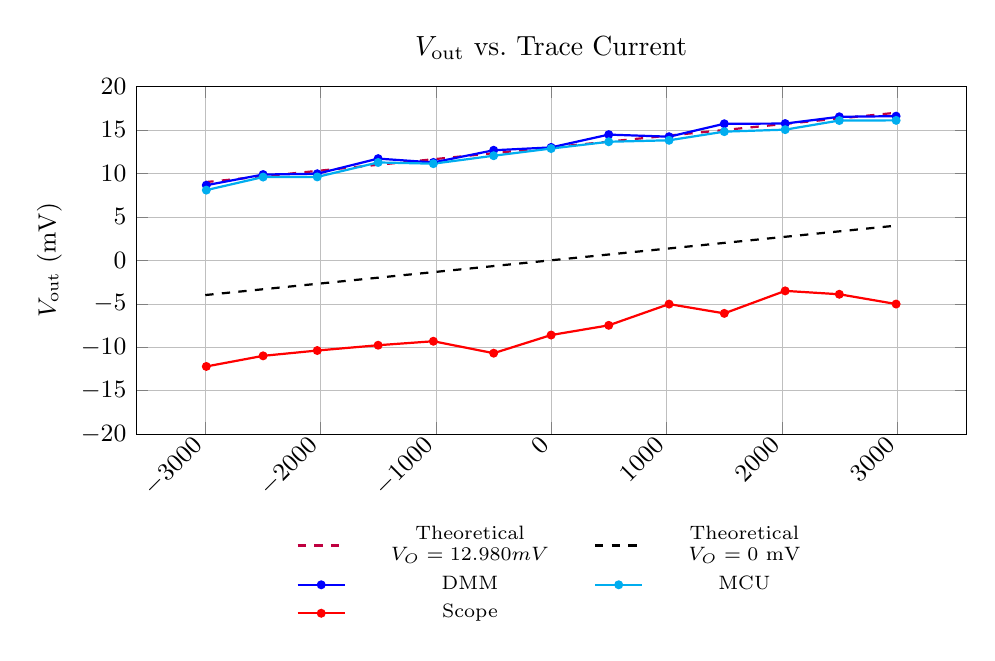
\begin{tikzpicture}
            \begin{axis}[
                width=\textwidth,
                height=6cm,
                title={$V_{\text{out}}$ vs.\ Trace Current},
                xlabel={Trace current, $I$ (mA)},
                ylabel={$V_{\text{out}}$ (mV)},
                grid=both,
                grid style={line width=.1pt, draw=gray!20},
                major grid style={line width=.2pt, draw=gray!50},
                mark size=1.2pt,
                xtick={-3000,-2000,-1000,0,1000,2000,3000},
                x tick label style={rotate=45, anchor=east},
                /pgf/number format/1000 sep={},
                label style={font=\small},
                tick label style={font=\small},
                legend style={
                    at={(0.5,-0.23)},
                    anchor=north,
                    font=\scriptsize,
                    legend columns=2,
                    /tikz/column sep=0.5cm,
                    draw=none
                },
          ymin=-20,
ymax=20,
ytick={-20,-15,-10,-5,0,5,10,15,20},
            ]

                % ------------------------------------------------
                % Theoretical response
                %
                % CT100 sensitivity = 4.5 mV/V/mT
                % VDD = 3.30 V
                % Analytical field coefficient = 0.0892 mT/A (d = 1.77 mm)
                %
                % dV/dI = 4.5 x 3.32 x 0.0892 = 1.332 mV/A
                %       = 1.645 mV/A
                %
                % 12.980 mV is used only as a visual intercept
                % to compare slope with the measured response.
                % ------------------------------------------------
                \addplot[
                    color=purple,
                    dashed,
                    thick,
                    domain=-3000:3000,
                    samples=100
                ]
                {12.980+1.332*(x/1000)};

\addlegendentry{\shortstack{Theoretical \\ $V_O = 12.980mV$}}

                \addplot[
                    color=black,
                    dashed,
                    thick,
                    domain=-3000:3000,
                    samples=100
                ]
                {1.332*(x/1000)};
           \addlegendentry{\shortstack{Theoretical \\ $V_O = 0\text{ mV}$}}

                % ------------------------------------------------
                % DMM Data
                % ------------------------------------------------
                \addplot[
                    color=blue,
                    thick,
                    mark=*
                ]
                coordinates {
                    (-2991.0, 8.634)
                    (-2498.5, 9.860)
                    (-2029.0, 9.950)
                    (-1501.0, 11.690)
                    (-1022.0, 11.250)
                    (-499.0, 12.650)
                    (-0.7, 12.980)
                    (499.0, 14.450)
                    (1022.0, 14.210)
                    (1501.0, 15.697)
                    (2029.0, 15.720)
                    (2498.5, 16.500)
                    (2991.0, 16.570)
                };
                \addlegendentry{DMM}

                % ------------------------------------------------
                % MCU Data
                % ------------------------------------------------
                \addplot[
                    color=cyan,
                    thick,
                    mark=*
                ]
                coordinates {
                    (-2991.0, 8.069)
                    (-2498.5, 9.571)
                    (-2029.0, 9.584)
                    (-1501.0, 11.249)
                    (-1022.0, 11.107)
                    (-499.0, 12.022)
                    (-0.7, 12.847)
                    (499.0, 13.628)
                    (1022.0, 13.796)
                    (1501.0, 14.790)
                    (2029.0, 15.020)
                    (2498.5, 16.068)
                    (2991.0, 16.088)
                };
                \addlegendentry{MCU}

                % ------------------------------------------------
                % Scope Data
                % ------------------------------------------------
                \addplot[
                    color=red,
                    thick,
                    mark=*
                ]
                coordinates {
                    (-2991.0, -12.207)
                    (-2498.5, -10.986)
                    (-2029.0, -10.376)
                    (-1501.0, -9.766)
                    (-1022.0, -9.308)
                    (-499.0, -10.681)
                    (-0.7, -8.594)
                    (499.0, -7.477)
                    (1022.0, -5.035)
                    (1501.0, -6.104)
                    (2029.0, -3.516)
                    (2498.5, -3.906)
                    (2991.0, -5.030)
                };
                \addlegendentry{Scope}

            \end{axis}
        \end{tikzpicture}

        \captionof{figure}{
            Voltage cross-validation during the non-irradiated, unshielded
            current sweep. The dashed lines shows the theoretical CT100
            responses.
        }
        \label{fig:voltage-cross-val}

    \end{minipage}%
    \hfill
    % ============================================================
    % RIGHT: Current Cross-Validation
    % ============================================================
    \begin{minipage}[t]{0.48\textwidth}
        \centering

        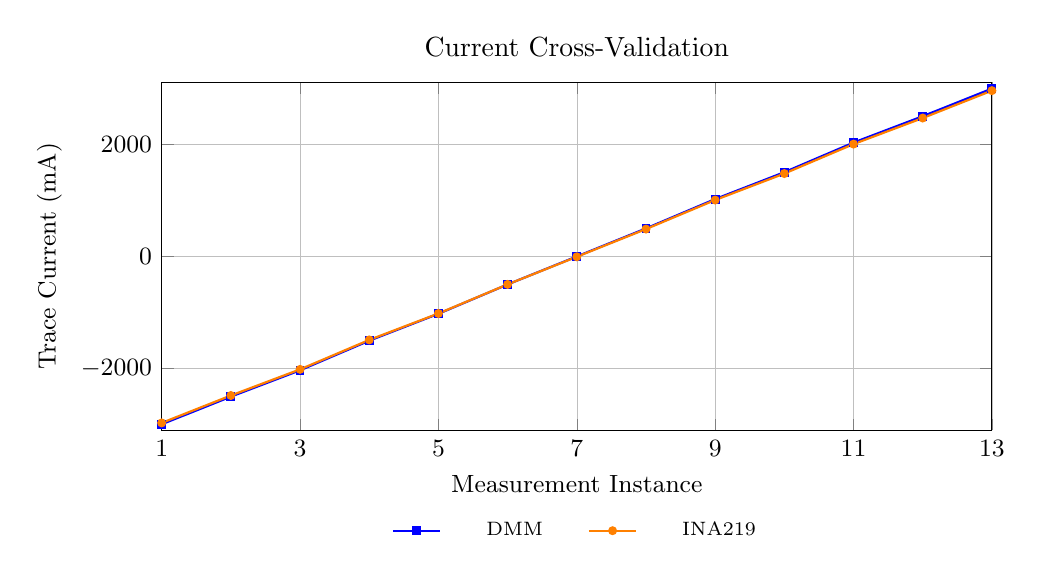
\begin{tikzpicture}
            \begin{axis}[
                width=\textwidth,
                height=6cm,
                title={Current Cross-Validation},
                xlabel={Measurement Instance},
                ylabel={Trace Current (mA)},
                grid=both,
                grid style={line width=.1pt, draw=gray!20},
                major grid style={line width=.2pt, draw=gray!50},
                mark size=1.2pt,
                xmin=1,
                xmax=13,
                xtick={1,3,5,7,9,11,13},
                /pgf/number format/1000 sep={},
                label style={font=\small},
                tick label style={font=\small},
                legend style={
                    at={(0.5,-0.23)},
                    anchor=north,
                    font=\scriptsize,
                    legend columns=2,
                    /tikz/column sep=0.5cm,
                    draw=none
                },
                ymin=-3100,
                ymax=3100
            ]

                % ------------------------------------------------
                % DMM Current
                % ------------------------------------------------
                \addplot[
                    color=blue,
                    thick,
                    mark=square*
                ]
                coordinates {
                    (1,-2991.0)
                    (2,-2498.5)
                    (3,-2029.0)
                    (4,-1501.0)
                    (5,-1022.0)
                    (6,-499.0)
                    (7,-0.7)
                    (8,499.0)
                    (9,1022.0)
                    (10,1501.0)
                    (11,2029.0)
                    (12,2498.5)
                    (13,2991.0)
                };
                \addlegendentry{DMM}

                % ------------------------------------------------
                % INA219 Current
                % ------------------------------------------------
                \addplot[
                    color=orange,
                    thick,
                    mark=*
                ]
                coordinates {
                    (1,-2966.7)
                    (2,-2478.2)
                    (3,-2012.6)
                    (4,-1487.7)
                    (5,-1016.6)
                    (6,-498.2)
                    (7,-6.3)
                    (8,487.8)
                    (9,1005.2)
                    (10,1477.2)
                    (11,2002.1)
                    (12,2466.4)
                    (13,2954.8)
                };
                \addlegendentry{INA219}



            \end{axis}
        \end{tikzpicture}

        \captionof{figure}{
            Current cross-validation across the 13-point sweep. 
        }
        \label{fig:current-cross-val}

    \end{minipage}
\end{figure}

The theoretical current-to-voltage gradient at $V_{\text{DD}} = \SI{3.32}{\volt}$ is $\SI{1.332}{\milli\volt\per\ampere}$ (Equation~\eqref{eq:ct100-voltage-current-slope}). The measured DMM gradient ($1.356 \pm \SI{0.067}{\milli\volt\per\ampere}$) is 101.8\% of this value and the MCU gradient ($1.315 \pm \SI{0.055}{\milli\volt\per\ampere}$) is 98.7\%; both differences are smaller than the standard error of the fit. Expressed as sensitivities these are 4.58 and $\SI{4.44}{\milli\volt\per\volt\per\milli\tesla}$, close to the datasheet typical value of 4.5. The tolerance on the sensor's height in its package (Section~\ref{sec:field-model}) gives a predicted gradient of 1.27 to $\SI{1.43}{\milli\volt\per\ampere}$ ($-5\%$ to $+7\%$), so the measurement agrees with the model within both the measurement and the model uncertainty.

\subsection{Instrumentation Validation}
\label{sec:instr-validation}

The sweep also compares the three instruments, using Figure~\ref{fig:voltage-cross-val} for voltage and Figure~\ref{fig:current-cross-val} for current.

\textbf{Voltage.} The DMM and MCU readings track one another closely: across the 13 points the mean difference is about $\SI{0.5}{\milli\volt}$ and the largest is $\SI{0.9}{\milli\volt}$, less than one ADC step ($\SI{1.61}{\milli\volt}$). The oscilloscope disagreed with both, showing a current-dependent response that went negative. A likely cause is that its two channels are referenced to separate ground clips, so ground-return drops that grow with the trace current appear differently on each channel before they are subtracted. Because the DMM and MCU agree, the oscilloscope was not used for any later DC measurement. It was kept for transients, where its time resolution is needed.

\textbf{Current.} The INA219 tracked the DMM with a near-unity relationship across the full sweep, with a largest difference of $\SI{36.2}{\milli\ampere}$. Because the INA219 is part of the board, it was used as the current reference for all later sweeps, which removed the need to log the DMM alongside it and shortened each test.

The saturation events were also found to move the zero-field baseline of the sensor. This is quantified in a dedicated before-and-after test in Section~\ref{sec:hysteresis}, and its consequences are discussed in Section~\ref{sec:disc-hysteresis}.



\section{Radiation Testing (Total Ionising Dose)}
\label{sec:radiation-testing}

\subsection{Rationale and Test Isolation Strategy}
\label{sec:rad-rationale}

Crystalline MgO, the MTJ's insulating barrier, is expected to be far more tolerant of ionising radiation than the amorphous SiO\textsubscript{2} used in conventional silicon devices (Section~\ref{sec:rad-tolerance-lit}). Only the CT100 sensors were irradiated, not the boards, so that any change could be attributed to the sensor rather than to the microcontroller, regulator or current monitor, which are conventional silicon devices and more likely to be affected.


\subsection{Experimental Setup}
\label{sec:rad-setup}

Ten CT100 sensors were exposed using a \SI{320}{\kilo\volt} tube potential (tungsten target, \SI{30}{\degree} anode angle, \SI{3}{\milli\metre} beryllium filter) at a beam current of \SI{10}{\milli\ampere}. The beam was seasoned (ramped up to full parameters) from 15:55 to 16:05 NZST on 22 July 2026, and held at full \SI{320}{\kilo\volt}/\SI{10}{\milli\ampere} output until switch-off at 19:26 NZST, giving \SI{3}{\hour}~\SI{21}{\minute} (\SI{12060}{\second}) of full-power exposure.

The sensors were irradiated unpowered, with all pins floating, before being soldered to any board. \todo{Confirm this is how they were irradiated.} The dose rate at the sensors was calculated as $\SI{0.0338}{\gray\per\second}$ in silicon ($\SI{3.38}{rad(Si)\per\second}$), by approximating the beam path as $\SI{315}{\milli\metre}$ of air followed by $\SI{5}{\milli\metre}$ of aluminium and modelling the sensor as a block of silicon. Over the $\SI{12060}{\second}$ of full-power exposure this gives a total dose of $\SI{407.6}{\gray}$, or $\SI{40.76}{\kilo rad}$(Si). This figure is an estimate rather than a measured dose. The calculation approximates the beam path and treats the packaged sensor as pure silicon, whereas the die sits inside a mould compound with metal leads that also absorb and scatter X-rays, and the dose was not confirmed with a dosimeter at the sensor position. The lower dose received during the ten-minute ramp-up is not included, so the figure slightly underestimates the total. \todo{If the facility's dosimetry or dose calculation gives an uncertainty, state it here, e.g.\ $\pm$x\%.}

\begin{figure}[H]
    \centering
    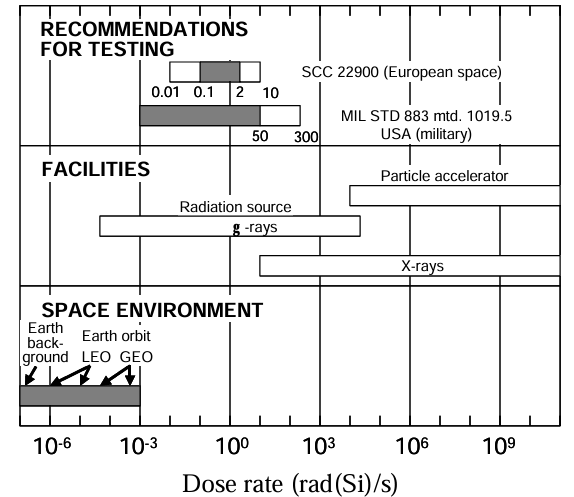
\includegraphics[width=0.7\textwidth]{rad_testing_spec}
    \caption{ Comparison of the dose rates found in
the radiation environments and the rates used in the testing of components
for tolerance.}
    \label{fig:rad_testing_spec}
\end{figure}

To place this exposure in context, Figure~\ref{fig:rad_testing_spec} compares the dose rates found in space with those used for testing, following the radiation hardness assurance framework of Poivey \cite{poivey_rha}. Natural environments such as low Earth orbit and geostationary orbit deliver dose at very low, continuous rates, below $10^{-3}$~rad(Si)/s, so ground tests use much higher rates to accumulate a mission dose in hours. The rate used here, $\SI{3.38}{rad(Si)\per\second}$ ($\SI{12.2}{\kilo rad}$(Si)/h), lies inside the standard-rate window of 3.6 to $\SI{36}{\kilo rad}$/h (1 to $\SI{10}{rad\per\second}$) of the European total-dose test method, ESCC 22900 \cite{escc22900}. The test was not, however, an ESCC 22900 test: that method specifies a cobalt-60 gamma or electron-accelerator source rather than X-rays, and it requires parts to be held at their worst-case bias throughout exposure \cite{escc22900}. The result therefore shows whether this dose causes a measurable permanent change in the tested sensors under these conditions; it is not a qualification of the part for flight.


\subsection{Sensor-Only Board Saturation Response Post-Irradiation}
\label{sec:rad-sensoronly-response}

To evaluate whether radiation exposure alters sensor saturation limits or transient recovery dynamics, two irradiated units (Samples 3 and 4) were driven to magnetic saturation following the methodology established in Section~\ref{sec:standalone-sat-recovery}. Table~\ref{tab:sat-ceiling-all} summarizes the saturation ceilings, baseline offsets, differential swings, and recovery times across all eight trials for both non-irradiated and irradiated sample groups for comparison.

Figure~\ref{fig:scope-irradiated} shows the oscilloscope captures for the irradiated samples. Following the same trace colour assignment used in the non-irradiated characterization, the blue waveform ($M_1$) represents the differential output voltage ($V_{\text{out}} = X_1 - X_2$), while the yellow ($C_1$) and green ($C_2$) waveforms represent the individual $X_1$ and $X_2$ bridge terminal voltages, respectively.
 


\begin{table}[h]
\centering
\caption{Saturation ceiling and recovery time two irradiated/non-irradiated samples for comparison.}
\label{tab:sat-ceiling-all}
\begin{tabular}{@{}llrrrr@{}}
\toprule
Sample  & Ceiling (V) & Baseline (mV) & Swing $\Delta V$ (V) & Recovery (ms) \\
\midrule
1   & $-1.126$ & $-17.4$ & $1.108$ & 76.5 \\
1   & $+1.125$ & $-12.5$ & $1.138$ & 74.0 \\
2 & $-1.145$ & $-17.4$ & $1.128$ & 76.0 \\
2   & $+1.125$ & $-12.5$ & $1.138$ & 67.5 \\
3       & $-1.131$ & $-22.3$ & $1.108$ & 70.5 \\
3       & $+1.111$ & $-12.5$ & $1.123$ & 65.5 \\
4      & $-1.145$ & $-22.3$ & $1.123$ & 78.0 \\
4       & $+1.111$ & $-22.3$ & $1.133$ & 85.0 \\

\bottomrule
\end{tabular}
\end{table}


\begin{figure}[H]
    \centering
    % Top Row: Sample 3
    \begin{subfigure}[b]{0.48\textwidth}
        \centering
        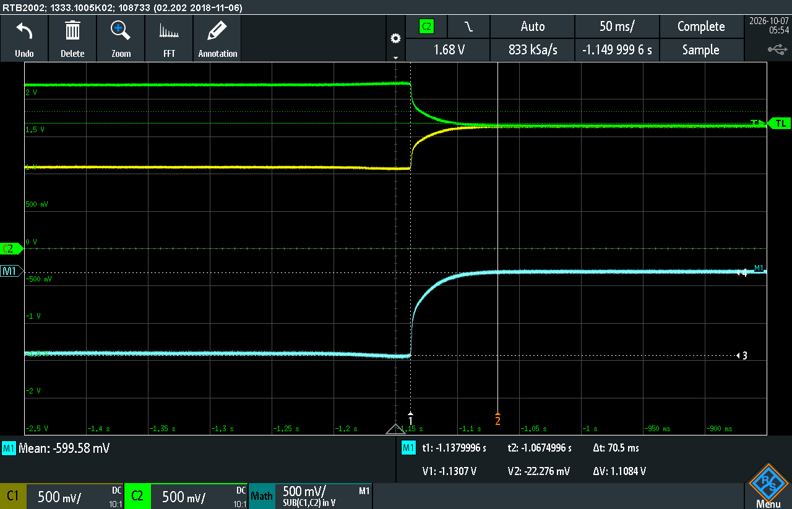
\includegraphics[width=\textwidth]{3_satn.png}
        \caption{Sample 3: Negative Saturation Recovery}
        \label{fig:3_satn}
    \end{subfigure}
    \hfill
    \begin{subfigure}[b]{0.48\textwidth}
        \centering
        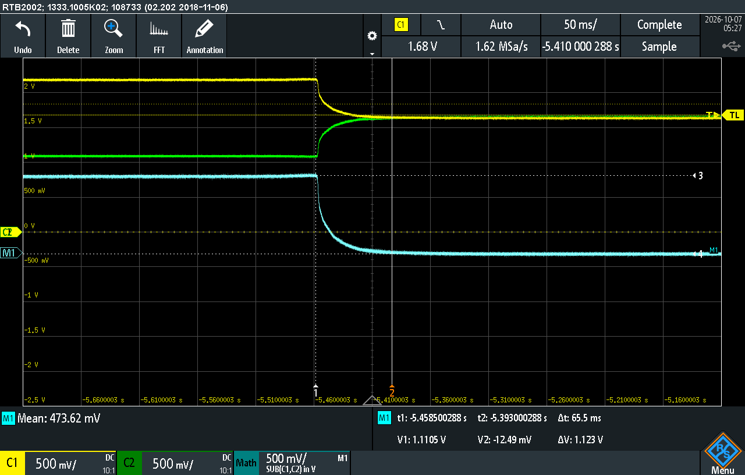
\includegraphics[width=\textwidth]{3_satp.png}
        \caption{Sample 3: Positive Saturation Recovery}
        \label{fig:3_satp}
    \end{subfigure}
    
    \vspace{0.4cm}
    
    % Bottom Row: Sample 4
    \begin{subfigure}[b]{0.48\textwidth}
        \centering
        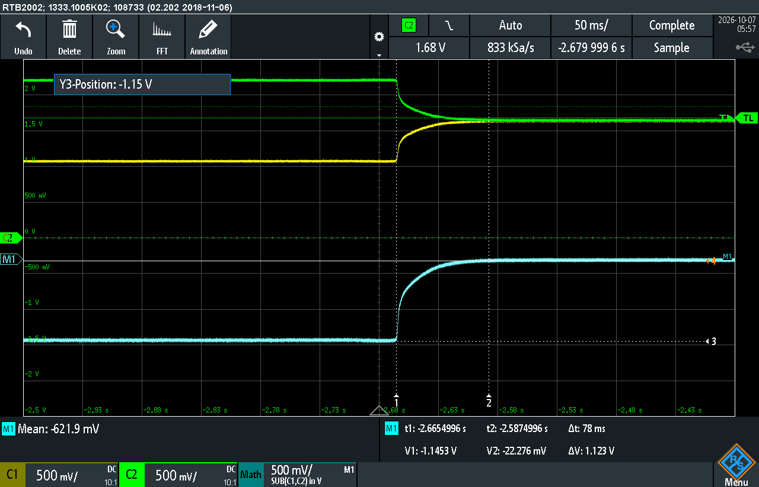
\includegraphics[width=\textwidth]{4_satn.png}
        \caption{Sample 4: Negative Saturation Recovery}
        \label{fig:4_satn}
    \end{subfigure}
    \hfill
    \begin{subfigure}[b]{0.48\textwidth}
        \centering
        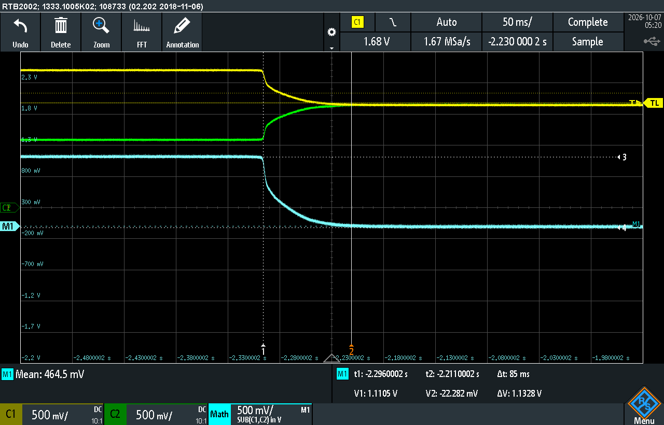
\includegraphics[width=\textwidth]{4_satp.png}
        \caption{Sample 4 ): Positive Saturation Recovery}
        \label{fig:4_satp}
    \end{subfigure}
    
    \caption{Oscilloscope captures displaying post-irradiation saturation voltage clamping and transient relaxation trajectories for irradiated sensor board Samples 3 and 4 across both field polarities.}
    \label{fig:scope-irradiated}
\end{figure}

Averaging across both polarities and units within each group, the non-irradiated group exhibits a mean saturation ceiling of $\SI{1.130}{\volt}$ compared to $\SI{1.124}{\volt}$ for the irradiated group, representing a $0.5\%$ difference. The mean recovery time across groups is $\SI{73.5}{\milli\second}$ non-irradiated versus $\SI{74.75}{\milli\second}$ irradiated, a $1.7\%$ difference.

The differences between the groups (0.5\% in ceiling and 1.7\% in recovery time) are smaller than the differences between the two non-irradiated units themselves, whose ceilings differ by up to 1.8\% and whose recovery times differ by up to $\SI{9}{\milli\second}$ (Table~\ref{tab:sat-ceiling-all}). The irradiated sensors therefore show no detectable permanent change in ceiling or recovery at the tested dose. Both groups were tested in the same session on 7 October 2026, so the comparison is not affected by session-to-session variation.


\subsection{Quantitative Sweep on the Integrated Board}
\label{sec:rad-sweep}

After irradiation, one sensor was soldered to an integrated board and the current sweep of Section~\ref{sec:sensitivity-fit} was repeated; the results are listed in Table~\ref{tab:sensitivity-irr}. This sensor had never been exposed to a saturating field, before or after irradiation, so its sweep is free of the offset shift described in Section~\ref{sec:hysteresis}.

\begin{figure}[H]
    \centering
    
    % Left side: The Table (Slightly wider for 3 columns)
    \begin{minipage}[c]{0.42\textwidth}
        \centering
        \small % Keeps the text size compact
        \captionof{table}{Irradiated sample current sweep.}
        \label{tab:sensitivity-irr}
        \begin{tabular}{@{}rrr@{}}
            \toprule
            Current (mA) & DMM (mV) & MCU (mV) \\
            \midrule
            \(-2999.0\) & \(-3.723\) & \(-3.258\) \\
            \(-2595.0\) & \(-3.123\) & \(-2.803\) \\
            \(-1999.0\) & \(-2.570\) & \(-1.748\) \\
            \(-1512.0\) & \(-1.620\) & \(-0.044\) \\
            \(-1017.0\) & \(-1.050\) & \(-0.001\) \\
            \(-498.0\) & \(-0.100\) & $0.463$ \\
            \(-0.7\) & $0.269$ & $0.308$ \\
            $498.0$ & $1.130$ & $1.749$ \\
            $1017.0$ & $1.640$ & $2.657$ \\
            $1512.0$ & $2.098$ & $3.178$ \\
            $1999.0$ & $2.720$ & $3.298$ \\
            $2595.0$ & $3.303$ & $4.350$ \\
            $2999.0$ & $3.912$ & $4.834$ \\
            \bottomrule
        \end{tabular}
    \end{minipage}%
    \hfill
    % Right side: The Plot (Dual lines)
    \begin{minipage}[c]{0.55\textwidth}
        \centering
        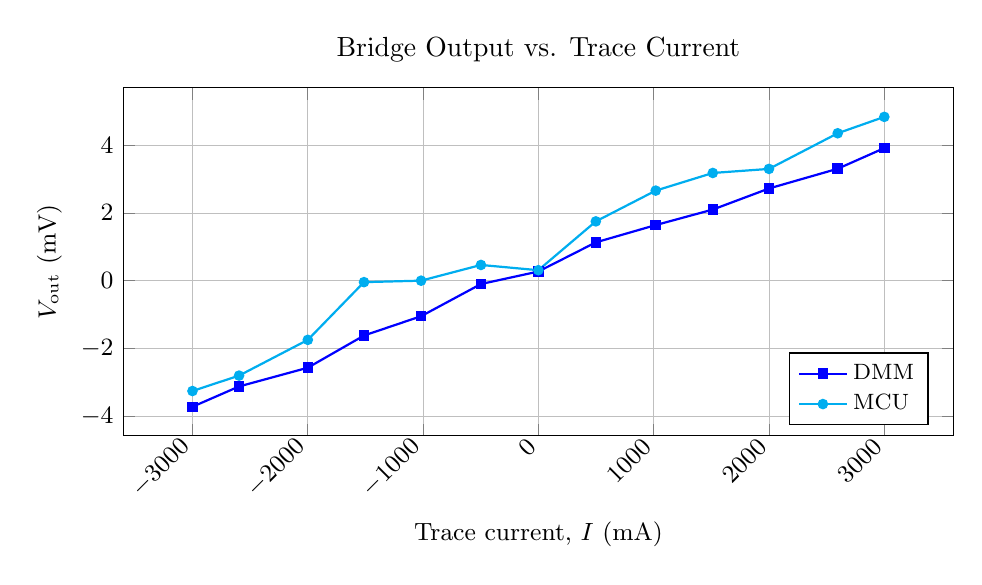
\begin{tikzpicture}
            \begin{axis}[
                width=\textwidth,
                height=6cm, % Squashes vertical height
                title={Bridge Output vs. Trace Current},
                xlabel={Trace current, $I$ (mA)},
                ylabel={$V_{\text{out}}$ (mV)},
                grid=both,
                grid style={line width=.1pt, draw=gray!20},
                major grid style={line width=.2pt, draw=gray!50},
                mark size=1.5pt,
                x tick label style={rotate=45, anchor=east},
                /pgf/number format/1000 sep={},
                label style={font=\small},
                tick label style={font=\small},
                legend pos=south east, % Puts legend in bottom right corner
                legend style={font=\footnotesize, cells={anchor=west}}
            ]
                % First line: DMM Data
                \addplot[color=blue, thick, mark=square*] coordinates {
                    (-2999.0, -3.723) (-2595.0, -3.123) (-1999.0, -2.570)
                    (-1512.0, -1.620) (-1017.0, -1.050) (-498.0, -0.100)
                    (-0.7, 0.269) (498.0, 1.130) (1017.0, 1.640)
                    (1512.0, 2.098) (1999.0, 2.720) (2595.0, 3.303) (2999.0, 3.912)
                };
                \addlegendentry{DMM}

                % Second line: MCU Data
                \addplot[color=cyan, thick, mark=*] coordinates {
                    (-2999.0, -3.258) (-2595.0, -2.803) (-1999.0, -1.748)
                    (-1512.0, -0.044) (-1017.0, -0.001) (-498.0, 0.463)
                    (-0.7, 0.308) (498.0, 1.749) (1017.0, 2.657)
                    (1512.0, 3.178) (1999.0, 3.298) (2595.0, 4.350) (2999.0, 4.834)
                };
                \addlegendentry{MCU}
            \end{axis}
        \end{tikzpicture}
        \captionof{figure}{Plot of irradiated DMM and MCU sweeps detailed in Table~\ref{tab:sensitivity-irr}.}
        \label{fig:sensitivity-irr-dual-plot}
    \end{minipage}
\end{figure}

The same linear fit gives $1.269 \pm \SI{0.026}{\milli\volt\per\ampere}$ on the DMM ($R^2 = 0.995$) and $1.312 \pm \SI{0.063}{\milli\volt\per\ampere}$ on the MCU ($R^2 = 0.975$), which are 93.6\% and 99.8\% of the non-irradiated values (Section~\ref{sec:sensitivity-fit}). The DMM difference of 6.4\% is somewhat larger than the 4\% session-to-session variation (Section~\ref{sec:session-variance}) but only 1.2 times the combined standard error of the two fits, and the MCU shows no change at all, so the two instruments do not agree on any change. No significant change in gradient was found at the tested dose, consistent with the junction-level results in Section~\ref{sec:rad-tolerance-lit}. Because the comparison is between two different sensors, a change smaller than the unit-to-unit spread in gradient could not be detected.

\subsection{Irradiated Saturation Recovery on the Integrated Board}
\label{sec:sat-recovery-irradiated}

Following the \SI{40.76}{\kilo rad}(Si) Total Ionizing Dose (TID) exposure, the saturation recovery of the integrated board was evaluated with a regulator input of $V_{\text{CC}} = \SI{5.00}{\volt}$ and a measured TMR sensor supply of $V_{\text{DD}} = \SI{3.289}{\volt}$, the irradiated board was subjected to the same magnetic saturation procedure as in Section~\ref{sec:sat-recovery-integrated}. The resulting recovery waveforms are plotted in Figure~\ref{fig:integrated-recovery-sat} and the key metrics are summarized in Table~\ref{tab:sat-ceiling-iradl}. The following irradiated data was collected on the 9th of October 2026. 


\begin{table}[H]
\centering
\caption{Saturation recovery results, irradiated integrated board (Board B).}
\label{tab:sat-ceiling-iradl}
\begin{tabular}{@{}lrrrr@{}}
\toprule
Sample & Ceiling (V) & Baseline (mV) & Swing (V) & Recovery (ms) \\
\midrule
B & $-1.146$ & $0.0$ & 1.146 & 66.7 \\
B & $+1.149$ & $+1.6$ & 1.147 & 63.2 \\
\bottomrule
\end{tabular}
\end{table}


\begin{figure}[h]
\centering
\begin{tikzpicture}
\begin{groupplot}[
    group style={group size=2 by 2, horizontal sep=1.5cm, vertical sep=1.7cm},
    width=0.48\textwidth, height=0.36\textwidth,
    xmin=-20, xmax=150, grid=major, grid style={gray!25}, axis lines=box,
    tick label style={font=\footnotesize}, label style={font=\small}, title style={font=\small},
]
\nextgroupplot[title={(a) Irradiated, negative saturation recovery}, xlabel={Time since rising edge (ms)}, ylabel={$V_{\text{out}}$ (V)}, ymin=-1.3, ymax=0.2]
\addplot[red!70!black, thick] table[col sep=comma, x=t_ms, y=v_V] {rec_irr_neg.csv};
\draw[dashed] (axis cs:66.7,-1.3) -- (axis cs:66.7,0.2);
\node[font=\scriptsize, anchor=north west, fill=white, inner sep=1pt] at (axis cs:70,-0.55) {$t_{\text{rec}}=66.7$ ms};
\node[font=\scriptsize, anchor=west] at (axis cs:5,-1.1) {ceiling $-1.146$ V};

\nextgroupplot[title={(b) Irradiated, positive saturation recovery }, xlabel={Time since falling edge (ms)}, ymin=-0.2, ymax=1.3]
\addplot[red!70!black, thick] table[col sep=comma, x=t_ms, y=v_V] {rec_irr_pos.csv};
\draw[dashed] (axis cs:63.2,-0.2) -- (axis cs:63.2,1.3);
\node[font=\scriptsize, anchor=south west, fill=white, inner sep=1pt] at (axis cs:66,0.45) {$t_{\text{rec}}=63.2$ ms};
\node[font=\scriptsize, anchor=west] at (axis cs:3,1.1) {ceiling $+1.149$ V};
\end{groupplot}
\end{tikzpicture}
\caption{Irradiated Saturation recovery on the integrated board after the magnet is removed, for both field directions. }
\label{fig:integrated-recovery-sat}
\end{figure}



\section{Magnetic Shielding}
\label{sec:shielding}

\subsection{Enclosure Design}
\label{sec:shielding-enclosure}

The enclosure frame was 3D printed in PLA. To check that the printed frame does not affect the field at the sensor, its relative permeability $\mu_r$ was estimated from published measurements of its magnetic susceptibility $\chi$. The susceptibility describes how strongly a material magnetises in an applied field $H$ where the magnetisation is given by $M = \chi H$. The flux density in the material is then:
\begin{equation}
B = \mu_0 (H + M) = \mu_0 (1 + \chi) H,
\label{eq:susceptibility}
\end{equation}
and comparing this with the definition $B = \mu_0 \mu_r H$ gives:
\begin{equation}
\mu_r = 1 + \chi .
\label{eq:mur-chi}
\end{equation}
Sangal et al. measured the susceptibility of common 3D printing polymers and found all of them to be weakly diamagnetic, with $\chi$ between about $-8.1$ and $-8.7$ parts per million (ppm) for PLA, PETG and ABS \cite{sangal2023}. One part per million is $10^{-6}$, so for PLA, with $\chi \approx -8.3$~ppm,
\begin{equation}
\mu_r = 1 + \chi = 1 + \left(-8.3 \times 10^{-6}\right) \approx 0.9999917 .
\label{eq:mur-pla}
\end{equation}

This differs from the permeability of free space ($\mu_r = 1$) by less than 0.001\%, so the printed frame has no measurable effect on the field at the sensor. It serves only to hold the ferrite plates and the board in place; all of the shielding comes from the ferrite and nanocrystalline layers.

 Surrounding a sensor with a high-permeability material gives magnetic flux a low-reluctance path around the enclosed volume, so an external field is partly diverted away from the sensor. For an ideal closed spherical shell of inner radius $a$, thickness $t \ll a$ and relative permeability $\mu_r \gg 1$, the field inside is reduced by a factor of about $1 + 2\mu_r t/(3a)$ \cite{fitzpatrick_shielding}. A constant ambient field adds only a fixed offset to the output, so shielding is expected to reduce that offset and any noise or drift it causes, not to change the gradient of the response to the trace current (Section~\ref{sec:disc-shielding}).

Mu-metal, an 80\% nickel--iron--molybdenum alloy, is the usual choice for DC and low-frequency shielding because of its very high permeability: for fully annealed material the initial relative permeability is about 50{,}000 at DC and 100{,}000 at \SI{60}{\hertz}, with a maximum of about 350{,}000 and a saturation flux density of \SI{0.74}{\tesla} \cite{msc_mumetal}. It was not used here because of its cost.

Instead, a MnZn ferrite, TDK (EPCOS) SIFERRIT material N95, was selected as a cost-effective alternative. The manufacturer quotes an initial relative permeability $\mu_i$ of 3000 at $25^{\circ}\text{C}$ and a saturation flux density $B_S$ of \SI{525}{\milli\tesla} at $25^{\circ}\text{C}$ \cite{tdk_n95}. Six N95 slabs, each \SI{100}{\milli\metre} $\times$ \SI{100}{\milli\metre} $\times$ \SI{5}{\milli\metre}, form the walls of the enclosure. With $\mu_r = 3000$, $t = \SI{5}{\milli\metre}$ and an inner radius of about \SI{50}{\milli\metre}, the closed-shell expression above gives an ideal shielding factor near 200, so a closed shell would cut an external field by about two orders of magnitude. This is an upper bound: the quoted permeability is a small-signal value for a ferrite core rather than a measurement at DC in an enclosure, and the real enclosure has seams and a cable cut-out. The ambient fields to be attenuated (tens of microtesla) are far below the \SI{525}{\milli\tesla} saturation flux density, so the ferrite stays in its linear region.

Power and data reach the enclosed board through an ST-Link programmer, so a cut-out was designed into the enclosure for the cable. Any gap raises the reluctance of the shield's flux path and lets ambient flux leak in towards the sensor.

To reduce this flux leakage, the cut-out was covered with a flexible nanocrystalline shielding foil (YNTECH NF, Qingdao Yunlu Energy Technology). The manufacturer describes its nanocrystalline material as an Fe-based soft magnetic material with a high saturation flux density and a permeability about ten times that of ferrite \cite{yunlu_nanocrystalline}, but gives no specific values for this foil. Measured with a digital caliper, the foil is $\SI{0.11}{\milli\metre}$ thick including its protective plastic film and about $\SI{0.02}{\milli\metre}$ thick with the film removed. The second value is close to the caliper's $\SI{0.01}{\milli\metre}$ resolution, so it is approximate.

Figure~\ref{fig:shielding_enclosure} shows the enclosure at three stages: the printed chassis, the board mounted inside (Figure~\ref{fig:box_pcb}), and the final wrapped assembly (Figure~\ref{fig:box_nano}).


\begin{figure}[H]
    \centering
    % Define the professional style: Bright cyan lines, clean white badges
    \tikzset{
        badge/.style={fill=white, draw=black!40, thick, rounded corners=2pt, inner sep=3pt, font=\sffamily\small\bfseries, text=black!80},
        pointer/.style={-stealth, draw=cyan, line width=1.5pt}
    }

    % Subfigure A: CAD Model
    \begin{subfigure}[b]{0.32\textwidth}
        \centering
        \begin{tikzpicture}
            \node[anchor=south west, inner sep=0] (imageA) at (0,0) {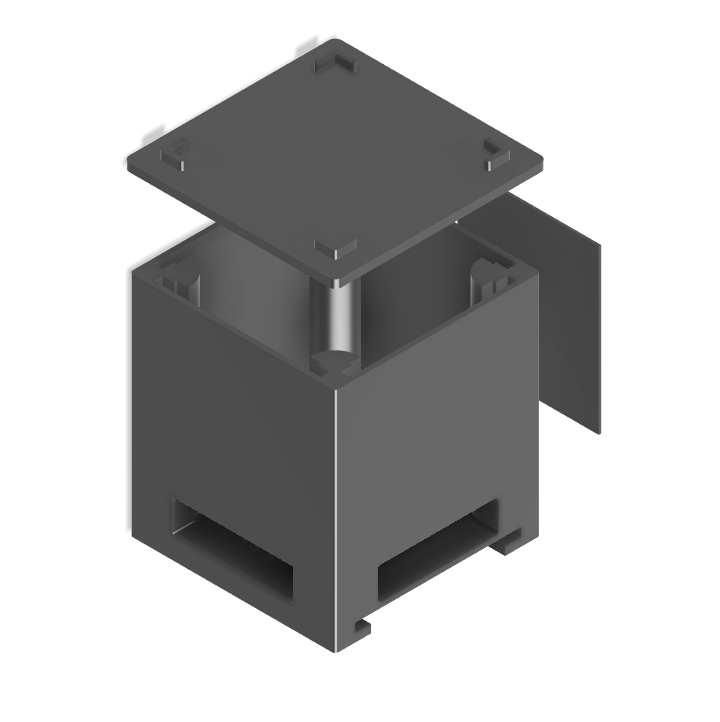
\includegraphics[width=\textwidth]{Box_FINAL_v2 v1.png}};
            \begin{scope}[x={(imageA.south east)},y={(imageA.north west)}]
                % F badge pointing precisely to the bottom right ferrite insertion slot
                \node[badge] (F_cad) at (0.85, 0.1) {F};
                \draw[pointer] (F_cad) -- (0.7, 0.25);
            \end{scope}
        \end{tikzpicture}
        \caption{Enclosure CAD render.}
        \label{fig:box_cad}
    \end{subfigure}
    \hfill
    % Subfigure B: PCB inside the box
    \begin{subfigure}[b]{0.32\textwidth}
        \centering
        \begin{tikzpicture}
            \node[anchor=south west, inner sep=0] (imageB) at (0,0) {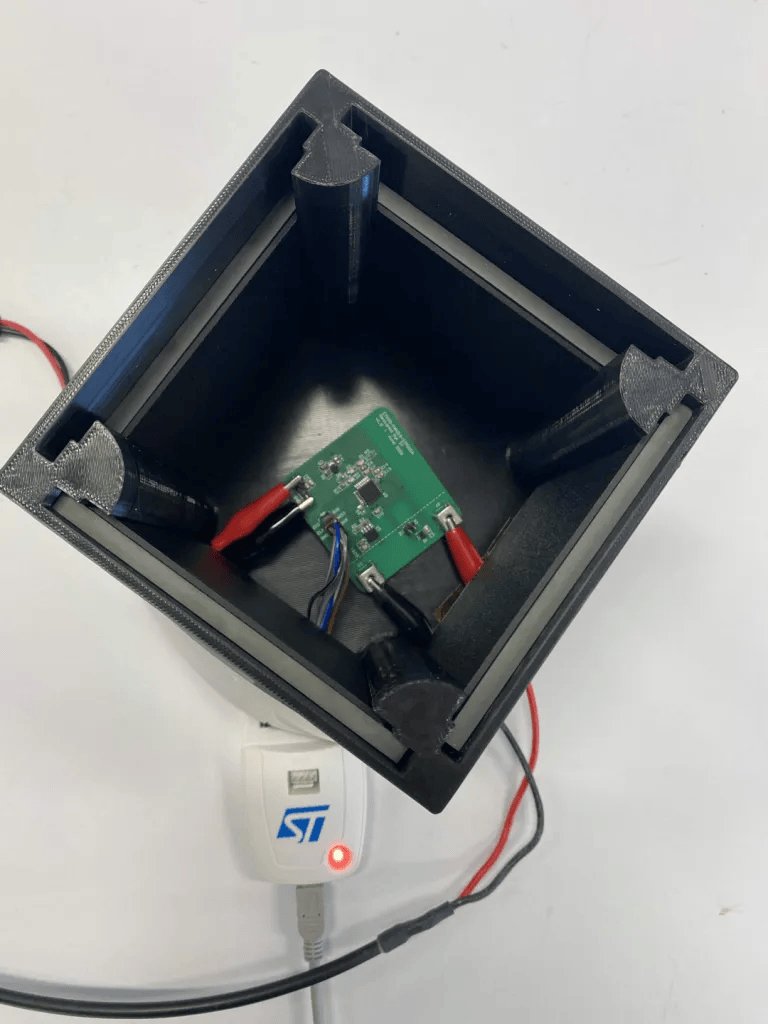
\includegraphics[width=\textwidth]{pcb_box.png}};
            \begin{scope}[x={(imageB.south east)},y={(imageB.north west)}]
                % F badge pointing exactly to the 4 internal ferrite slabs/slots
                \node[badge] (F_pcb) at (0.15, 0.85) {F};
                \draw[pointer] (F_pcb) -- (0.64, 0.73); % Top right slab
                \draw[pointer] (F_pcb) -- (0.80, 0.50); % Bottom right slab
                \draw[pointer] (F_pcb) -- (0.28, 0.40); % Bottom left slab
                \draw[pointer] (F_pcb) -- (0.3, 0.72); % Top left slab
            \end{scope}
        \end{tikzpicture}
        \caption{Internal PCB mounting.}
        \label{fig:box_pcb}
    \end{subfigure}
    \hfill
    % Subfigure C: Fully shielded with Nano/Ferrite layer
    \begin{subfigure}[b]{0.32\textwidth}
        \centering
        \begin{tikzpicture}
            \node[anchor=south west, inner sep=0] (imageC) at (0,0) {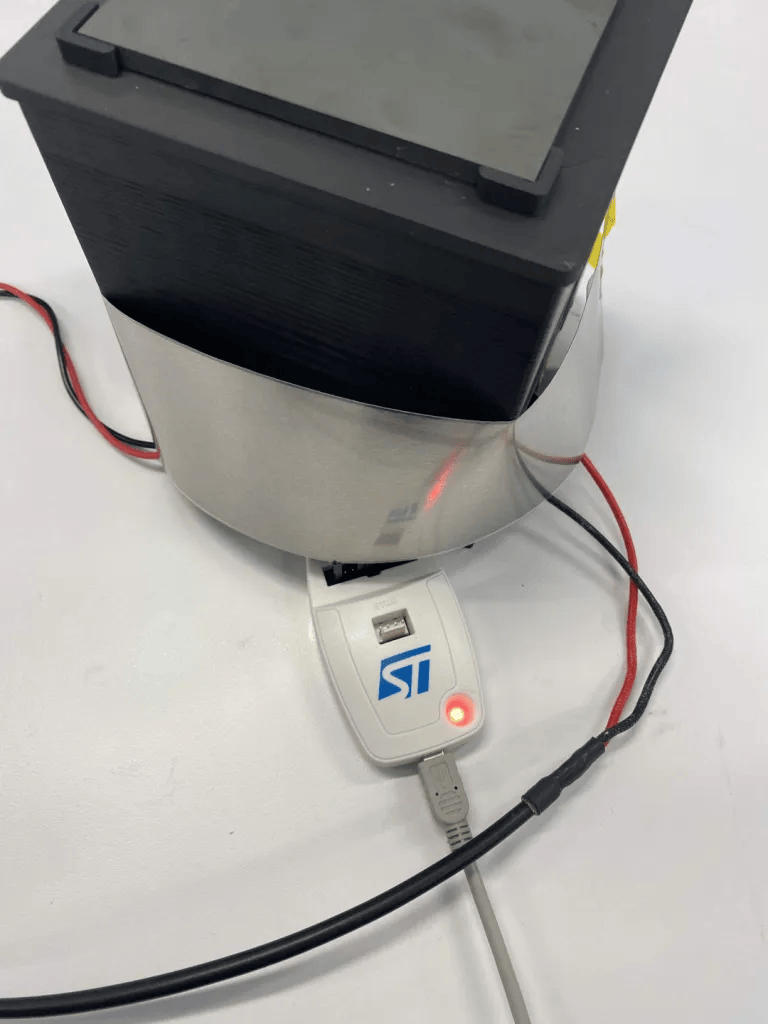
\includegraphics[width=\textwidth]{box_nano.png}};
            \begin{scope}[x={(imageC.south east)},y={(imageC.north west)}]
                % F badge pointing to the top ferrite lid block
                \node[badge] (F_ext) at (0.2, 0.8) {F};
                \draw[pointer] (F_ext) -- (0.55, 0.9);
                
                % N badge pointing directly onto the shiny metal shielding wrap
                \node[badge] (N_ext) at (0.85, 0.2) {N};
                \draw[pointer] (N_ext) -- (0.65, 0.550);
            \end{scope}
        \end{tikzpicture}
        \caption{Exterior shielding layer.}
        \label{fig:box_nano}
    \end{subfigure}
    
    \caption{Development of the magnetic shielding enclosure. (a) The 3D-printed chassis. (b) The integrated sensor board mounted inside. (c) The assembled test configuration wrapped in shielding. Annotations indicate the placement of ferrite plates (\textbf{F}) and flexible nanocrystalline shielding (\textbf{N}).} 
    \label{fig:shielding_enclosure}
\end{figure}
    

\subsection{Shielded Sweep Results}
\label{sec:shielded-results}

Because the MCU and DMM had already been shown to agree across the full current range (Section~\ref{sec:instr-validation}), the shielded sweeps were logged with the MCU alone. Leaving out the DMM also avoided routing extra leads into the enclosure, which would have complicated the setup and added another possible source of stray field. The non-irradiated and irradiated integrated boards were swept inside the enclosure with the same procedure as in Section~\ref{sec:nonirr-characterisation}. The irradiated sensor had still not been driven into saturation at this point.

The raw measurement data for both the non-irradiated and irradiated shielded sweeps are detailed in Table~\ref{tab:sensitivity-shielded} and Table~\ref{tab:sensitivity-irr-shielded}, respectively. To visualize the effect of the magnetic shielding, Figure~\ref{fig:shielding-overlay} compares these shielded sweeps directly against their unshielded counterparts.

These sweeps were performed at $V_{\text{DD}} = \SI{3.29}{\volt}$.



\begin{table}[H]
    \centering
    
    % --- ROW 1: CAPTIONS ---
    % Both minipages top-aligned [t] so the caption text starts at the exact same height
    \begin{minipage}[t]{0.48\textwidth}
        \caption{Shielded, non-irradiated current sweep (MCU only): bridge output vs.\ trace current.}
        \label{tab:sensitivity-shielded}
    \end{minipage}\hfill
    \begin{minipage}[t]{0.48\textwidth}
        \caption{Irradiated, shielded current sweep (MCU only): bridge output vs.\ trace current.}
        \label{tab:sensitivity-irr-shielded}
    \end{minipage}
    
    \vspace{0.3cm} % Small vertical buffer between captions and the tables
    
    % --- ROW 2: TABLES ---
    % Both minipages top-aligned [t] so the tables start at the exact same height
    \begin{minipage}[t]{0.48\textwidth}
        \centering
        \small
        \begin{tabular}{@{}rr@{}}
            \toprule
            Current (mA) & MCU (mV) \\
            \midrule
            \(-3043.4\) & 8.039 \\
            \(-2522.5\) & 8.549 \\
            \(-2057.7\) & 9.594 \\
            \(-1540.3\) & 9.949 \\
            \(-1040.2\) & 11.170 \\
            \(-546.2\) & 11.319 \\
            \(-6.3\) & 12.705 \\
            $535.4$ & 12.946 \\
            $996.2$ & 13.931 \\
            $1523.0$ & 14.530 \\
            $2038.1$ & 15.532 \\
            $2486.1$ & 16.103 \\
            $2988.7$ & 16.474 \\
            \bottomrule
        \end{tabular}
    \end{minipage}\hfill
    \begin{minipage}[t]{0.48\textwidth}
        \centering
        \small 
        \begin{tabular}{@{}rr@{}}
            \toprule
            Current (mA) & MCU (mV) \\
            \midrule
            \(-3007.1\) & \(-3.287\) \\
            \(-2501.2\) & \(-2.769\) \\
            \(-2054.6\) & \(-1.130\) \\
            \(-1567.3\) & 0.069 \\
            \(-1037.7\) & \(-0.001\) \\
            \(-532.1\) & 0.107 \\
            \(-6.3\) & 1.318 \\
            $512.5$ & 1.699 \\
            $1011.4$ & 2.837 \\
            $1557.8$ & 3.241 \\
            $2048.6$ & 3.933 \\
            $2560.6$ & 4.807 \\
            $3025.4$ & 4.932 \\
            \bottomrule
        \end{tabular}
    \end{minipage}
    
\end{table}


% ============================================================
% Preamble (if not already present):
%   \usepackage{pgfplots}
%   \usepgfplotslibrary{groupplots}
%   \pgfplotsset{compat=1.18}
% ============================================================
% Shielded vs. unshielded overlaid on ONE figure, one panel per
% sample condition. Both panels use the same vertical SPAN (14 mV)
% so the gradients can be compared by eye even though the two
% boards sit at different baselines. Raw MCU data, no table needed
% (the tables already exist elsewhere in the report).

\begin{figure}[h]
\centering
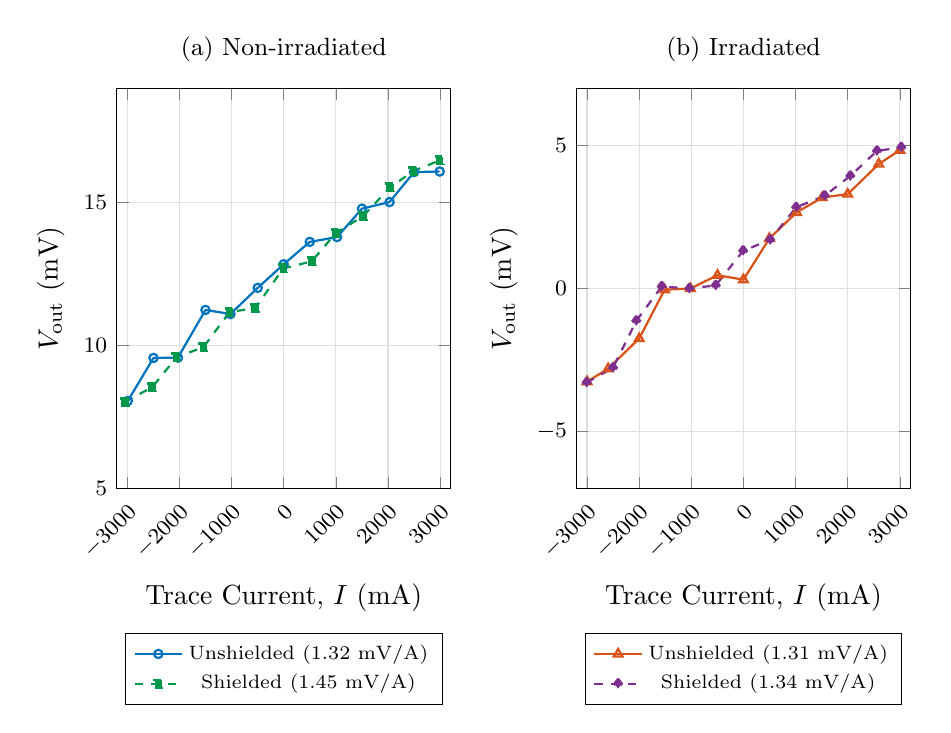
\begin{tikzpicture}
\begin{groupplot}[
    group style={group size=2 by 1, horizontal sep=1.6cm},
    width=0.48\textwidth, height=0.55\textwidth,
    xlabel={Trace Current, $I$ (mA)},
    ylabel={$V_{\text{out}}$ (mV)},
    xmin=-3200, xmax=3200,
    xtick={-3000,-2000,-1000,0,1000,2000,3000},
    xticklabel style={rotate=45, anchor=north east, /pgf/number format/1000 sep={}},
    tick label style={font=\footnotesize},
    label style={font=\small}, title style={font=\small},
    grid=major, grid style={gray!25},
    axis lines=box,
    legend style={font=\scriptsize, draw=black, at={(0.5,-0.36)}, anchor=north, legend columns=1},
]


            

% ---------------- Panel (a): non-irradiated ----------------
\nextgroupplot[title={(a) Non-irradiated},    ylabel={$V_{\text{out}}$ (mV)}, ymin=5, ymax=19]
\addplot[color={rgb,255:red,0;green,115;blue,189}, mark=o, mark size=1.5pt, thick]
    coordinates {
    (-2991.0,8.069) (-2498.5,9.571) (-2029.0,9.584) (-1501.0,11.249)
    (-1022.0,11.107) (-499.0,12.022) (-0.7,12.847) (499.0,13.628)
    (1022.0,13.796) (1501.0,14.790) (2029.0,15.020) (2498.5,16.068)
    (2991.0,16.088)};
\addlegendentry{Unshielded (1.32 mV/A)}
\addplot[color={rgb,255:red,0;green,153;blue,76}, mark=square*, mark size=1.4pt, thick, dashed]
    coordinates {
    (-3043.4,8.039) (-2522.5,8.549) (-2057.7,9.594) (-1540.3,9.949)
    (-1040.2,11.170) (-546.2,11.319) (-6.3,12.705) (535.4,12.946)
    (996.2,13.931) (1523.0,14.530) (2038.1,15.532) (2486.1,16.103)
    (2988.7,16.474)};
\addlegendentry{Shielded (1.45 mV/A)}

% ---------------- Panel (b): irradiated ----------------
\nextgroupplot[title={(b) Irradiated}, ymin=-7, ymax=7]
\addplot[color={rgb,255:red,217;green,83;blue,25}, mark=triangle, mark size=1.8pt, thick]
    coordinates {
    (-2999.0,-3.258) (-2595.0,-2.803) (-1999.0,-1.748) (-1512.0,-0.044)
    (-1017.0,-0.001) (-498.0,0.463) (-0.7,0.308) (498.0,1.749)
    (1017.0,2.657) (1512.0,3.178) (1999.0,3.298) (2595.0,4.350)
    (2999.0,4.834)};
\addlegendentry{Unshielded (1.31 mV/A)}
\addplot[color={rgb,255:red,125;green,46;blue,143}, mark=diamond*, mark size=1.8pt, thick, dashed]
    coordinates {
    (-3007.1,-3.287) (-2501.2,-2.769) (-2054.6,-1.130) (-1567.3,0.069)
    (-1037.7,-0.001) (-532.1,0.107) (-6.3,1.318) (512.5,1.699)
    (1011.4,2.837) (1557.8,3.241) (2048.6,3.933) (2560.6,4.807)
    (3025.4,4.932)};
\addlegendentry{Shielded (1.34 mV/A)}

\end{groupplot}
\end{tikzpicture}
\caption{Shielded vs.\ unshielded current sweeps (MCU readings) for (a) the non-irradiated and (b) the irradiated sample.}
\label{fig:shielding-overlay}
\end{figure}

 Shielding changes the gradient by $+10\%$ on the non-irradiated board and $+2.3\%$ on the irradiated board.

\subsection{Session-to-Session Variance}
\label{sec:session-variance}

To measure the repeatability of the method, the shielded sweep on the non-irradiated board was repeated in a separate session, at $V_{\text{DD}} = \SI{3.29}{\volt}$. The data are listed in Table~\ref{tab:variance-new-data}, and Figure~\ref{fig:variance-overlay} plots them with the first shielded sweep to show how the offset and gradient changed between sessions.

\begin{figure}[H]
    \centering
    
    % --- LEFT SIDE: THE TABLE ---
    \begin{minipage}[c]{0.38\textwidth}
        \centering
        \small 
        \captionof{table}{Validation Sweep: Non-Irradiated Shielded Board}
        \label{tab:variance-new-data}
        
        \begin{tabular}{@{}cc@{}}
            \toprule
            INA Current (mA) & MCU (mV) \\
            \midrule
            \(-3046.47\) & 8.039 \\
            \(-2492.64\) & 8.595 \\
            \(-2009.76\) & 9.604 \\
            \(-1493.87\) & 10.014 \\
            \(-1037.81\) & 11.110 \\
            \(-507.16\) & 11.312 \\
            \(-4.58\) & 12.514 \\
            $494.27$ & 12.888 \\
            $1055.68$ & 13.579 \\
            $1515.83$ & 14.455 \\
            $2016.78$ & 14.890 \\
            $2487.65$ & 15.978 \\
            $3006.08$ & 16.192 \\
            \bottomrule
        \end{tabular}
    \end{minipage}\hfill
    % --- RIGHT SIDE: THE PLOT ---
    \begin{minipage}[c]{0.58\textwidth}
        \centering
        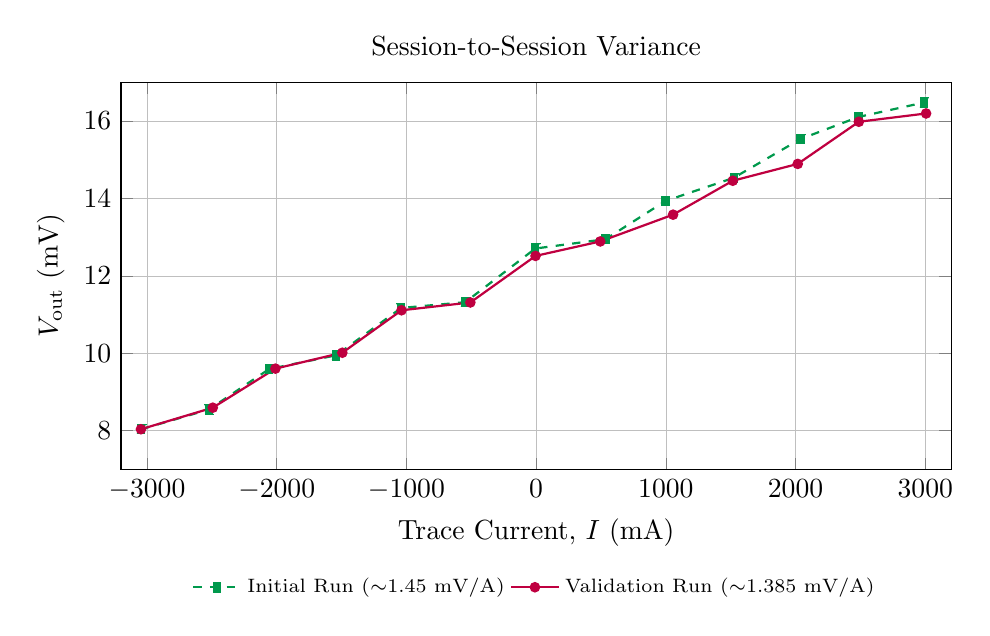
\begin{tikzpicture}
            \begin{axis}[
                width=\textwidth,
                height=6.5cm,
                title={Session-to-Session Variance},
                title style={align=center},
                xlabel={Trace Current, $I$ (mA)},
                ylabel={$V_{\text{out}}$ (mV)},
                grid=both,
                grid style={line width=.1pt, draw=gray!20},
                major grid style={line width=.2pt, draw=gray!50},
                xmin=-3200, xmax=3200,
                ymin=7, ymax=17,
                xtick={-3000,-2000,-1000,0,1000,2000,3000},
                /pgf/number format/1000 sep={},
                legend style={at={(0.5,-0.25)}, anchor=north, font=\scriptsize, legend columns=2, draw=none},
            ]
                
                % Initial Shielded Run
                \addplot[
                    color={rgb,255:red,0;green,153;blue,76}, 
                    mark=square*, mark size=1.5pt, thick, dashed
                ] coordinates {
                    (-3043.4,8.039) (-2522.5,8.549) (-2057.7,9.594) (-1540.3,9.949)
                    (-1040.2,11.170) (-546.2,11.319) (-6.3,12.705) (535.4,12.946)
                    (996.2,13.931) (1523.0,14.530) (2038.1,15.532) (2486.1,16.103)
                    (2988.7,16.474)
                };
                \addlegendentry{Initial Run (\(\sim\)1.45 mV/A)}

                % Validation Run (25/09)
                \addplot[
                    color=purple, 
                    mark=*, mark size=1.5pt, thick
                ] coordinates {
                    (-3046.47, 8.039) (-2492.64, 8.595) (-2009.76, 9.604) (-1493.87, 10.014)
                    (-1037.81, 11.110) (-507.16, 11.312) (-4.58, 12.514) (494.27, 12.888)
                    (1055.68, 13.579) (1515.83, 14.455) (2016.78, 14.890) (2487.65, 15.978)
                    (3006.08, 16.192)
                };
                \addlegendentry{Validation Run (\(\sim\)1.385 mV/A)}

            \end{axis}
        \end{tikzpicture}
        \captionof{figure}{Plots of two discrete testing sessions on the same shielded, non-irradiated board.}
        \label{fig:variance-overlay}
    \end{minipage}
    
\end{figure}

A linear fit to the validation sweep gives $1.385 \pm \SI{0.031}{\milli\volt\per\ampere}$. The first shielded run on the same board gave $1.446 \pm \SI{0.033}{\milli\volt\per\ampere}$ (Section~\ref{sec:shielded-results}), a difference of 4.2\% between two sessions under the same conditions, about 1.3 times their combined standard error. This is the session-to-session variation of the method.

This variation and the ADC step are the yardsticks for the two parts of H6. \textbf{Offset (H6a).} The fitted zero-current offset of the non-irradiated board was $\SI{12.60}{\milli\volt}$ unshielded and 12.39 and $\SI{12.25}{\milli\volt}$ in the two shielded runs, changes of $-0.21$ and $-\SI{0.35}{\milli\volt}$; on the irradiated board it moved from 1.00 to $\SI{1.21}{\milli\volt}$, a change of $+\SI{0.21}{\milli\volt}$ (Table~\ref{tab:all-fits}). All three changes are smaller than one ADC step and smaller than the largest change an ideal shield could cause (about $\SI{1}{\milli\volt}$), so the offset data cannot distinguish an effective shield from no shield. \textbf{Gradient (H6b).} On the irradiated board the gradient changed by $+2.3\%$, well within the session-to-session variation. On the non-irradiated board it changed by $+5.3\%$ or $+10.0\%$ depending on which shielded run is compared; the smaller value is close to the session-to-session variation and the larger is about twice it. The enclosure therefore does not clearly disturb the test field, although a small concentration of the trace field by the ferrite cannot be ruled out on the non-irradiated board.

\section{Quantitative Magnetic Hysteresis Testing}
\label{sec:hysteresis}


To isolate the effects of magnetic history from potential board-level hysteresis, the sensor on the non-irradiated integrated board was desoldered and replaced with a new sensor that had never been exposed to a magnetic field (Board C). All measurements were taken on 12 October 2026 with a regulator input of $V_{\text{CC}} = \SI{5.00}{\volt}$ and a sensor supply of $V_{\text{DD}} = \SI{3.321}{\volt}$.

The test was run in one session, with no other change to the board, in three steps: (i) a current sweep on the untouched sensor before saturation; (ii) saturation to the negative ceiling and then to the positive ceiling; and (iii) a second, identical current sweep after saturation. The two sweeps are listed in Tables~\ref{tab:naive-sat-before} and~\ref{tab:naive-sat-after} and plotted in Figure~\ref{fig:hysteresis-sweeps}. Panel (a) of that figure shows the raw output of both sweeps, and panel (b) shows them again with each sweep's fitted offset removed so that only the gradient is compared. The saturation events themselves are reported in Table~\ref{tab:mh-saturation} and Figure~\ref{fig:mh-recovery}.

\begin{figure}[H]
    \centering
    
    % ==========================================
    %       LEFT SIDE: STACKED TABLES
    % ==========================================
    \begin{minipage}[c]{0.40\textwidth}
        \centering
        \captionof{table}{Before Saturation}
        \label{tab:naive-sat-before}
        \small 
        \begin{tabular}{@{}rr@{}}
            \toprule
            INA (mA) & MCU (mV) \\
            \midrule
            $-3026.78$ & $-8.076$ \\
            $-2500.36$ & $-8.047$ \\
            $-2074.76$ & $-7.625$ \\
            $-1490.19$ & $-6.462$ \\
            $-1043.62$ & $-5.821$ \\
            $-508.79$  & $-4.869$ \\
            $-6.30$    & $-4.824$ \\
            $493.28$   & $-3.809$ \\
            $1003.71$  & $-3.222$ \\
            $1498.85$  & $-2.582$ \\
            $2037.68$  & $-1.641$ \\
            $2510.09$  & $-1.571$ \\
            $3025.05$  & $-0.709$ \\
            \bottomrule
        \end{tabular}
        
        \vspace{1.5cm} 
        
        \captionof{table}{After Saturation}
        \label{tab:naive-sat-after}
        \small 
        \begin{tabular}{@{}rr@{}}
            \toprule
            INA (mA) & MCU (mV) \\
            \midrule
            $-2971.20$ & $7.896$ \\
            $-2516.89$ & $8.091$ \\
            $-2031.67$ & $8.878$ \\
            $-1500.70$ & $9.660$ \\
            $-999.23$  & $10.051$ \\
            $-504.66$  & $11.124$ \\
            $-6.15$    & $11.297$ \\
            $492.07$   & $12.077$ \\
            $1010.23$  & $12.875$ \\
            $1504.07$  & $13.100$ \\
            $2039.39$  & $14.316$ \\
            $2502.52$  & $14.558$ \\
            $3018.47$  & $15.590$ \\
            \bottomrule
        \end{tabular}
    \end{minipage}\hfill
    % ==========================================
    %       RIGHT SIDE: STACKED PLOTS
    % ==========================================
    \begin{minipage}[c]{0.58\textwidth}
        \centering
        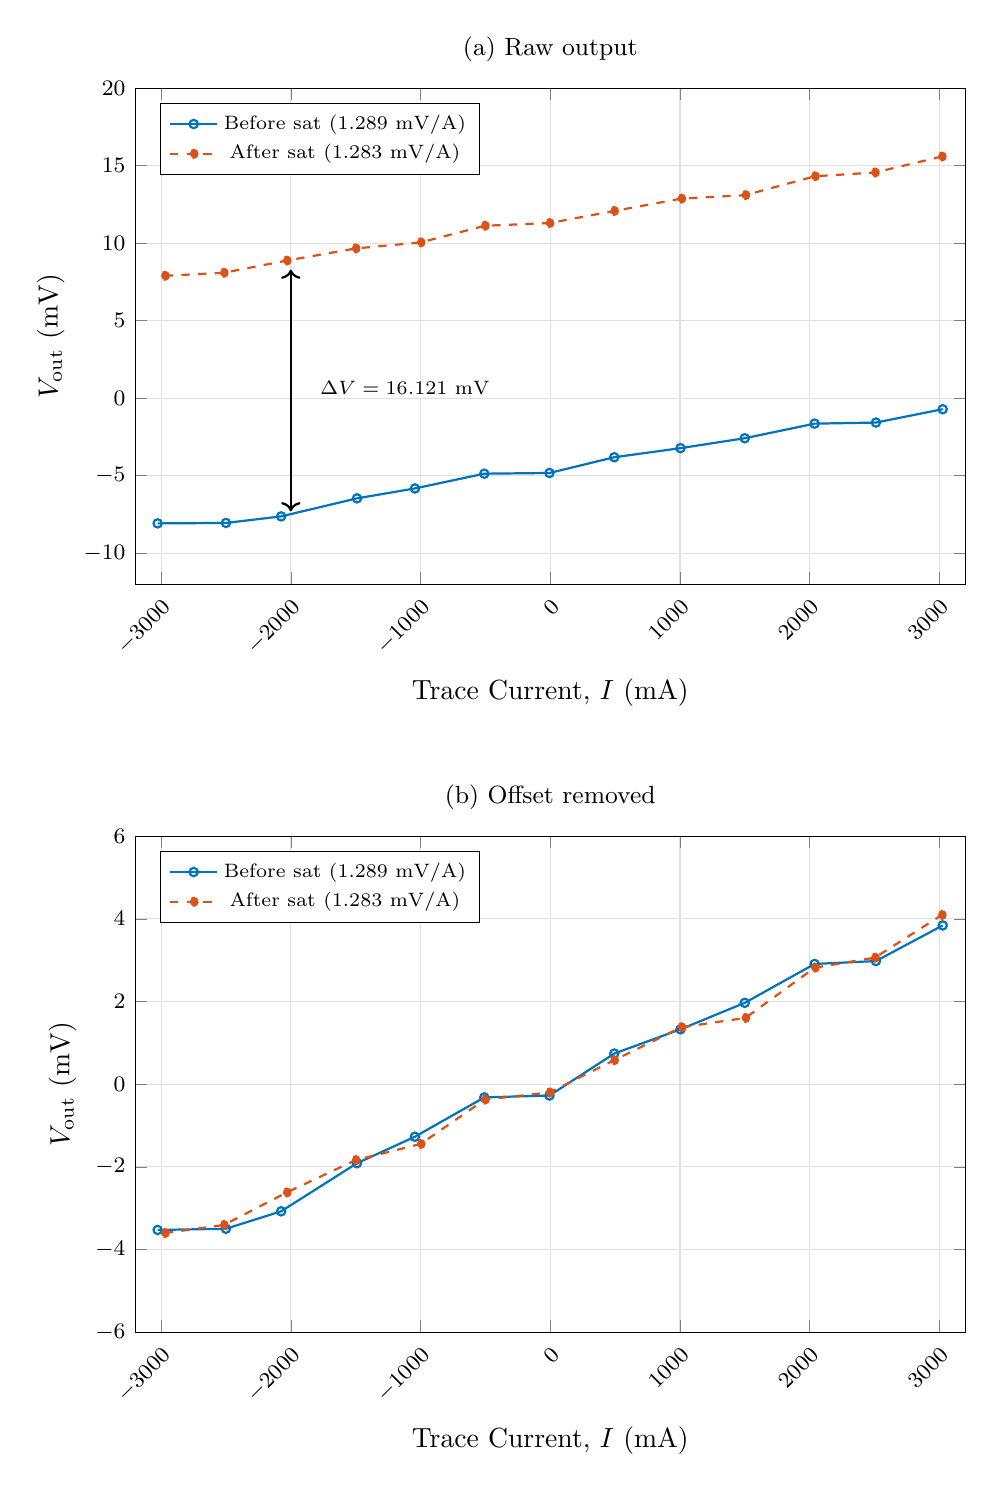
\begin{tikzpicture}
        \begin{groupplot}[
            group style={group size=1 by 2, vertical sep=3.2cm}, % <-- Increased vertical separation
            width=\textwidth, height=0.65\textwidth,
            xlabel={Trace Current, $I$ (mA)}, xmin=-3200, xmax=3200,
            xtick={-3000,-2000,-1000,0,1000,2000,3000},
            xticklabel style={rotate=45, anchor=north east, /pgf/number format/1000 sep={}},
            tick label style={font=\footnotesize}, label style={font=\small}, title style={font=\small},
            grid=major, grid style={gray!25}, axis lines=box,
        ]
        
        % Plot (a): Raw Output     xlabel={Trace Current, $I$ (mA)},
   % ylabel={$V_{\text{out}}$ (mV)},
        \nextgroupplot[
            title={(a) Raw output}, ylabel={$V_{\text{out}}$ (mV)}, ymin=-12, ymax=20,
            legend style={at={(0.03,0.97)}, anchor=north west, font=\scriptsize, legend columns=1} % <-- Moved to top left
        ]
        \addplot[color={rgb,255:red,0;green,115;blue,189}, mark=o, mark size=1.5pt, thick] coordinates {(-3026.8,-8.076) (-2500.4,-8.047) (-2074.8,-7.625) (-1490.2,-6.462) (-1043.6,-5.821) (-508.8,-4.869) (-6.3,-4.824) (493.3,-3.809) (1003.7,-3.222) (1498.9,-2.582) (2037.7,-1.641) (2510.1,-1.571) (3025.1,-0.709)};
        \addlegendentry{Before sat (1.289 mV/A)}
        
        \addplot[color={rgb,255:red,217;green,83;blue,25}, mark=*, mark size=1.4pt, thick, dashed] coordinates {(-2971.2,7.896) (-2516.9,8.091) (-2031.7,8.878) (-1500.7,9.660) (-999.2,10.051) (-504.7,11.124) (-6.1,11.297) (492.1,12.077) (1010.2,12.875) (1504.1,13.100) (2039.4,14.316) (2502.5,14.558) (3018.5,15.590)};
        \addlegendentry{After sat (1.283 mV/A)}
        
        \draw[<->, thick] (axis cs:-2000,-7.3) -- (axis cs:-2000,8.3);
        \node[font=\scriptsize, anchor=west, fill=white, inner sep=1pt] at (axis cs:-1800,0.65) {$\Delta V = 16.121$ mV};
         
        % Plot (b): Offset removed
        \nextgroupplot[
            title={(b) Offset removed}, ylabel={$V_{\text{out}}$ (mV)}, ymin=-6, ymax=6, 
            legend style={at={(0.03,0.97)}, anchor=north west, font=\scriptsize, legend columns=1} 
        ]
        \addplot[color={rgb,255:red,0;green,115;blue,189}, mark=o, mark size=1.5pt, thick] coordinates {(-3026.8,-3.526) (-2500.4,-3.497) (-2074.8,-3.075) (-1490.2,-1.912) (-1043.6,-1.271) (-508.8,-0.319) (-6.3,-0.274) (493.3,0.741) (1003.7,1.328) (1498.9,1.968) (2037.7,2.909) (2510.1,2.979) (3025.1,3.841)};
        \addlegendentry{Before sat (1.289 mV/A)} % <-- Added sensitivity for consistency
        
        \addplot[color={rgb,255:red,217;green,83;blue,25}, mark=*, mark size=1.4pt, thick, dashed] coordinates {(-2971.2,-3.601) (-2516.9,-3.406) (-2031.7,-2.619) (-1500.7,-1.837) (-999.2,-1.446) (-504.7,-0.373) (-6.1,-0.200) (492.1,0.580) (1010.2,1.378) (1504.1,1.603) (2039.4,2.819) (2502.5,3.061) (3018.5,4.093)};
        \addlegendentry{After sat (1.283 mV/A)} % <-- Added sensitivity for consistency
        
        \end{groupplot}
        \end{tikzpicture}
        
        \vspace{0.5cm}
        \captionof{figure}{Current sweep on a fresh, never-saturated sensor before (solid) and after (dashed) being driven to saturation. (a) Raw output: the curve moves up by $16.121$\,mV. (b) With offset removed, sweeps overlap.}
        \label{fig:hysteresis-sweeps}
    \end{minipage}
    
\end{figure}

\begin{table}[H]
\centering
\caption{Saturation recovery results, fresh sensor on the integrated board (Board C).}
\label{tab:mh-saturation}
\begin{tabular}{@{}lrrrr@{}}
\toprule
Sample & Ceiling (V) & Baseline (mV) & Swing (V) & Recovery (ms) \\
\midrule
C & $-1.107$ & $-1.6$ & 1.105 & 40.1 \\
C & $+1.117$ & $+11.3$ & 1.105 & 48.7 \\
\bottomrule
\end{tabular}
\end{table}



% ---------- Figure A: the two recovery transients ----------
\begin{figure}[H]
\centering
\begin{tikzpicture}
\begin{groupplot}[
    group style={group size=2 by 1, horizontal sep=1.5cm},
    width=0.48\textwidth, height=0.38\textwidth,
    xmin=-20, xmax=150, 
    grid=major, grid style={gray!25}, axis lines=box,
    tick label style={font=\footnotesize}, label style={font=\small}, title style={font=\small},
]
\nextgroupplot[title={(a) Negative saturation recovery}, ylabel={$V_{\text{out}}$ (V)}, ymin=-1.25, ymax=0.15,  xlabel={Time since rising edge (ms)},]
\addplot[blue!70!black, thick] table[col sep=comma, x=t_ms, y=v_V] {rec_mh_neg.csv};
\draw[dashed] (axis cs:40.1,-1.25) -- (axis cs:40.1,0.15);
\node[font=\scriptsize, anchor=north west, fill=white, inner sep=1pt] at (axis cs:44,-0.55) {$t_{\text{rec}}=40.1$ ms};
\node[font=\scriptsize, anchor=west] at (axis cs:58,-1.1) {ceiling $-1.107$ V};
 
\nextgroupplot[title={(b) Positive saturation recovery}, ymin=-0.15, ymax=1.25,  xlabel={Time since falling edge (ms)},]
\addplot[blue!70!black, thick] table[col sep=comma, x=t_ms, y=v_V] {rec_mh_pos.csv};
\draw[dashed] (axis cs:48.7,-0.15) -- (axis cs:48.7,1.25);
\node[font=\scriptsize, anchor=south west, fill=white, inner sep=1pt] at (axis cs:52,0.45) {$t_{\text{rec}}=48.7$ ms};
\node[font=\scriptsize, anchor=west] at (axis cs:58,1.1) {ceiling $+1.117$ V};
\end{groupplot}
\end{tikzpicture}
\caption{Newly Soldered Non-Irradiated Saturation recovery on the integrated board after the magnet is removed, for both field directions. }
\label{fig:mh-recovery}
\end{figure}


 When the saturating magnetic field is removed, the sensor output decays from its respective ceiling (-1.107 V for negative saturation, 1.117 V for positive saturation). Figure \ref{fig:mh-recovery} tracks this transient response, showing that the sensor settles to within 5 mV of its new baseline in 40.1 ms after the negative event, and 48.7 ms after the positive event.

The zero-field baseline is the output once the field has been removed. Table~\ref{tab:baseline-shift} lists the baseline before and after each saturation event for all three integrated boards, and Figure~\ref{fig:mh-baseline} shows the baseline of Board C through the sequence. ``Before'' is the median output in a quiet interval before the field was applied, ``after'' is the median output once recovery was complete, and the shift is after minus before, so a positive shift means the zero-field output moved up. The shifts are computed from unrounded values.

\begin{table}[H]
\centering
\caption{Baseline before and after each saturation event, integrated boards.}
\label{tab:baseline-shift}
\begin{tabular}{@{}llrrr@{}}
\toprule
Sample & Ceiling reached & Before (mV) & After (mV) & Shift (mV) \\
\midrule
A (non-irradiated) & Negative & $-6.4$ & $-8.1$ & $-1.6$ \\
A (non-irradiated) & Positive & $-8.1$ & $+12.9$ & $+20.9$ \\
B (irradiated) & Negative & $0.0$ & $0.0$ & $0.0$ \\
B (irradiated) & Positive & $0.0$ & $+1.6$ & $+1.6$ \\
C (fresh sensor) & Negative & $-4.8$ & $-1.6$ & $+3.2$ \\
C (fresh sensor) & Positive & $-1.6$ & $+11.3$ & $+12.9$ \\
\bottomrule
\end{tabular}
\end{table}

Three observations follow from Table~\ref{tab:baseline-shift}. First, on Board C the negative ceiling moved the baseline by only $+\SI{3.2}{\milli\volt}$ (two ADC steps of $\SI{1.61}{\milli\volt}$), but the positive ceiling that followed moved it by $+\SI{12.9}{\milli\volt}$, leaving the baseline at $+\SI{11.3}{\milli\volt}$, a total shift of $+\SI{16.1}{\milli\volt}$ from the untouched sensor. Second, Board A shows the same pattern, a negligible shift at the negative ceiling and a large one ($+\SI{20.9}{\milli\volt}$) at the positive ceiling. Third, the irradiated Board B shows no comparable shift ($0.0$ and $+\SI{1.6}{\milli\volt}$). Because the negative ceiling was always reached first, these data cannot yet separate the direction of the field from the order of the events, and Board B is a single irradiated unit.

\todo{Planned measurement: repeat this test on a second fresh sensor with the positive ceiling reached first, using the same session procedure. Add the two rows to Table~\ref{tab:baseline-shift} and state whether the large shift follows the field direction (positive ceiling) or the order of the events (second saturation).}

\textbf{Gradient stability.} Despite the shift in offset, the sensor's linear response to current is essentially unaffected. A straight-line fit to each sweep gives a gradient of $1.289 \pm 0.038$~mV/A before saturation and $1.283 \pm 0.030$~mV/A after, a change of only $-0.5\%$, which is far smaller than the standard error of either gradient. The fitted offset at zero current moves from $-4.55$~mV to $+11.50$~mV, a shift of $\SI{16.05}{\milli\volt}$, and $R^2$ stays above 0.99 (0.991 before and 0.994 after). Saturation therefore moves the whole response up without changing its slope or its linearity. This is the pattern seen in panel (b) of Figure~\ref{fig:hysteresis-sweeps}, where the two sweeps overlap once their offsets are removed.

 
% ---------- Figure B: baseline before, between and after the events ----------
\begin{figure}[H]
\centering
\begin{tikzpicture}
\begin{axis}[
    width=0.92\textwidth, height=0.32\textwidth,
    xlabel={Time (s)}, ylabel={$V_{\text{out}}$ (mV)}, xmin=0, xmax=29.5, ymin=-30, ymax=30,
    grid=major, grid style={gray!25}, axis lines=box,
    tick label style={font=\footnotesize}, label style={font=\small},
    unbounded coords=jump, restrict y to domain=-30:30,
]
\addplot[blue!70!black, thin] table[col sep=comma, x=t_s, y=v_mV] {trace_mh.csv};
\node[font=\scriptsize, fill=white, inner sep=1pt] at (axis cs:2.2,-18) {$-4.8$ mV};
\node[font=\scriptsize, fill=white, inner sep=1pt] at (axis cs:15,-18) {$-1.6$ mV};
\node[font=\scriptsize, fill=white, inner sep=1pt] at (axis cs:27,22) {$+11.3$ mV};
\end{axis}
\end{tikzpicture}
\caption{Output baseline before, between and after the two saturation events (view clipped to $\pm30$\,mV so the baseline is visible). The baseline moves from $-4.8$\,mV to $-1.6$\,mV after the negative saturation, then to $+11.3$\,mV after the positive saturation.}
\label{fig:mh-baseline}
\end{figure}
 

 

\section{Discussion}
\label{sec:discussion}

This project asked whether a low-cost commercial TMR sensor, the CT100, is operationally viable for CubeSat ADCS/EPS use, focusing on how it behaves when driven into saturation and after irradiation, as set out in Section~\ref{sec:research-question}. The motivation (Section~\ref{sec:intro}) is that CubeSat magnetometers must be small, light and low power, and that TMR offers high sensitivity in a few-millimetre package but has little space heritage (Section~\ref{sec:magnetometer-tech}). This section first checks that the test method can be trusted, then discusses each result against the literature and the CubeSat use case, and ends with the limitations of the work.

Table~\ref{tab:hypothesis-outcomes} summarises how the results answer the hypotheses of Section~\ref{sec:hypotheses}, and the subsections that follow discuss each one.

\begin{table}[H]
\centering
\caption{Outcome of each hypothesis.}
\label{tab:hypothesis-outcomes}
\small
\begin{tabular}{@{}>{\raggedright\arraybackslash}p{0.27\textwidth}>{\raggedright\arraybackslash}p{0.16\textwidth}>{\raggedright\arraybackslash}p{0.47\textwidth}@{}}
\toprule
Hypothesis & Outcome & Evidence \\
\midrule
H1: Ceiling at $\pm V_{\text{DD}}/3$ & Supported & Every ceiling within about 5\% of $V_{\text{DD}}/3$; positive and negative ceilings differ by 0.9 to 2.4\%. \\
H2: Gradient matches model & Supported & All nine fits lie within $-5\%$ to $+9\%$ of the predicted $\SI{1.332}{\milli\volt\per\ampere}$, equivalent to 4.3 to $\SI{4.9}{\milli\volt\per\volt\per\milli\tesla}$, inside the datasheet range of 3.8 to 5.2. \\
H3: Recovery within one \SI{10}{\hertz} sample & Partly supported & All recoveries (40 to $\SI{85}{\milli\second}$) are shorter than $\SI{100}{\milli\second}$, but the guard window with a safety factor (127.5 to $\SI{170}{\milli\second}$) is not, so 1 to 2 samples must be discarded. \\
H4: No lasting effect of saturation & Rejected & Baseline shifted by $\SI{16.1}{\milli\volt}$, ten ADC steps; gradient changed by only $-0.5\%$. \\
H5: No radiation effect & Supported for the tested units and dose & Ceiling (0.5\%) and recovery (1.7\%) differences smaller than the spread between non-irradiated units; gradient change at most 1.2 combined standard errors. Three units, one dose, unbiased exposure. \\
H6: Shielding & (a) Unresolved; (b) Partly supported & (a) Offset changed by $-0.35$ to $+\SI{0.21}{\milli\volt}$, below one ADC step and below the $\le\SI{1}{\milli\volt}$ expected. (b) Gradient changed by $+2.3\%$ (irradiated), within session variation, and $+5$ to $+10\%$ (non-irradiated), at or above it. \\
\bottomrule
\end{tabular}
\end{table}

\subsection{Validity of the Test Method}
\label{sec:disc-validity}

The results depend on the measurement chain, so it was validated before it was used. The MCU voltage readings agree with the DMM to within $\SI{0.9}{\milli\volt}$, less than one ADC step, and the INA219 current reading agrees with the DMM to within about 1 to 2\% (Section~\ref{sec:instr-validation}). The oscilloscope disagreed with both for DC measurements and was therefore used only for transients, where its time resolution matters. On that basis the MCU alone was used for the shielded sweeps and the hysteresis test, which saved a large amount of test time, while the radiation sweeps used both the DMM and the MCU so that they were directly comparable with the earlier baseline. Two further checks support the method. The field model, built only from the board stack-up and the datasheet position of the sensing element, predicts the measured gradients to within a few percent (Section~\ref{sec:sensitivity-fit}), and repeated sweeps on the same board agree within about 4\% (Section~\ref{sec:session-variance}). The method is therefore good enough for the effects reported here, which are offset shifts of 13 to $\SI{21}{\milli\volt}$ and gradient changes of a few percent. It is not good enough for signals at the level of Earth's field, as discussed in Section~\ref{sec:disc-limitations}.

\subsection{Field Model and Sensitivity}
\label{sec:disc-model}

Across the seven MCU sweeps the measured gradient lies between 1.283 and $\SI{1.446}{\milli\volt\per\ampere}$ (mean $\SI{1.33}{\milli\volt\per\ampere}$), and the two DMM sweeps give 1.269 and $\SI{1.356}{\milli\volt\per\ampere}$ (Table~\ref{tab:all-fits}). The field model predicts $\SI{1.332}{\milli\volt\per\ampere}$, so every fit lies within $-5\%$ to $+9\%$ of the prediction and the mean agrees to better than 1\% (Figure~\ref{fig:gradient-summary}). Expressed as sensitivities, the fits give 4.3 to $\SI{4.9}{\milli\volt\per\volt\per\milli\tesla}$, around the datasheet typical value of 4.5 and well inside its range of 3.8 to 5.2 \cite{ct100_datasheet}. Figure~\ref{fig:sensitivity-comparison} compares the four test conditions with each sweep's offset removed: all four lie on the theoretical line within their scatter.

This agreement depends on getting the geometry right. The model is most sensitive to the distance $d$ between the trace and the sensing element: a model that ignored the height of the sensing element inside its package ($d \approx \SI{0.42}{\milli\metre}$) would predict a gradient about 70\% higher than measured. With the datasheet sensor position, the remaining spread between sweeps (up to about 9\%) is comparable to the repeatability of one board (4\%, Section~\ref{sec:session-variance}), the standard error of each fit (2 to 5\%) and the tolerance on the sensor height ($-5\%$ to $+7\%$ in the predicted gradient). A constant ambient field cannot explain any of it, because it adds an offset without changing the gradient. For a CubeSat designer the result is that the datasheet sensitivity and a simple strip-conductor model are good enough to design a test or calibration coil to within about 10\%, although each flight unit would still be calibrated.

\begin{table}[H]
\centering
\caption{Linear fit of every current sweep: gradient with standard error, offset and $R^2$.}
\label{tab:all-fits}
\begin{tabular}{@{}lrrr@{}}
\toprule
Sweep & Gradient (mV/A) & Offset (mV) & $R^2$ \\
\midrule
Non-irradiated, unshielded (DMM) & $1.356 \pm 0.067$ & 13.09 & 0.974 \\
Non-irradiated, unshielded (MCU) & $1.315 \pm 0.055$ & 12.60 & 0.981 \\
Irradiated, unshielded (DMM) & $1.269 \pm 0.026$ & 0.22 & 0.995 \\
Irradiated, unshielded (MCU) & $1.312 \pm 0.063$ & 1.00 & 0.975 \\
Non-irradiated, shielded (MCU) & $1.446 \pm 0.033$ & 12.39 & 0.994 \\
Non-irradiated, shielded repeat (MCU) & $1.385 \pm 0.031$ & 12.25 & 0.995 \\
Irradiated, shielded (MCU) & $1.342 \pm 0.065$ & 1.21 & 0.975 \\
Fresh sensor, before saturation (MCU) & $1.289 \pm 0.038$ & $-4.55$ & 0.991 \\
Fresh sensor, after saturation (MCU) & $1.283 \pm 0.030$ & 11.50 & 0.994 \\
\bottomrule
\end{tabular}
\end{table}

\begin{figure}[H]
\centering
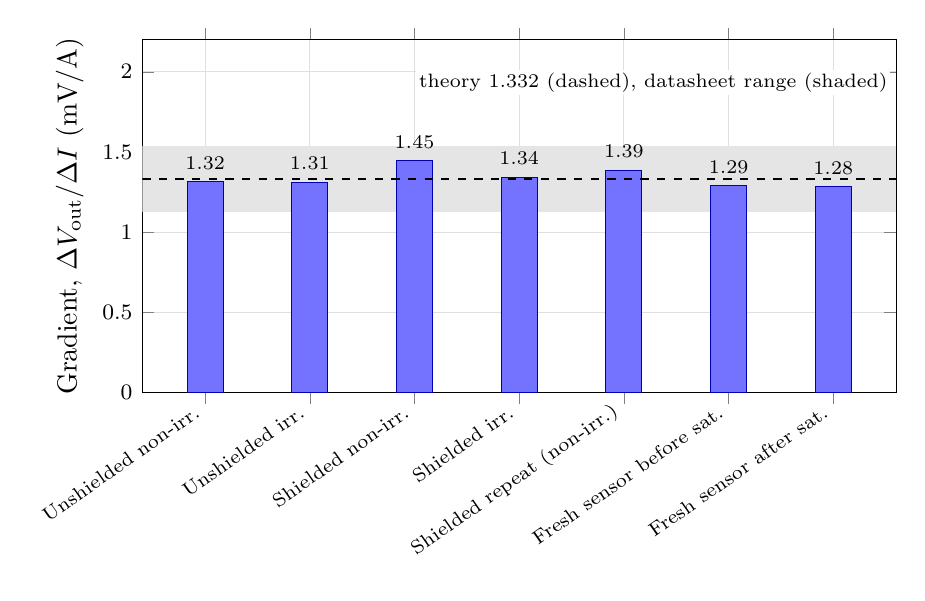
\begin{tikzpicture}
\begin{axis}[
    ybar, width=0.92\textwidth, height=0.5\textwidth, bar width=13pt,
    ymin=0, ymax=2.2, xmin=0.4, xmax=7.6,
    ylabel={Gradient, $\Delta V_{\text{out}}/\Delta I$ (mV/A)},
    xtick={1,2,3,4,5,6,7},
    xticklabels={Unshielded non-irr., Unshielded irr., Shielded non-irr., Shielded irr., Shielded repeat (non-irr.), Fresh sensor before sat., Fresh sensor after sat.},
    xticklabel style={rotate=35, anchor=east, font=\scriptsize},
    tick label style={font=\footnotesize}, label style={font=\small},
    grid=major, grid style={gray!25}, axis lines=box,
    nodes near coords,
    every node near coord/.append style={font=\scriptsize, yshift=1pt},
    /pgf/number format/.cd, fixed, precision=2,
]
\fill[gray!20] (axis cs:0.4,1.125) rectangle (axis cs:7.6,1.539);
\addplot[fill=blue!55, draw=blue!70!black] coordinates {(1,1.315) (2,1.312) (3,1.446) (4,1.342) (5,1.385) (6,1.289) (7,1.283)};
\draw[dashed, thick] (axis cs:0.4,1.332) -- (axis cs:7.6,1.332);
\node[font=\scriptsize, anchor=south east, fill=white, inner sep=1pt] at (axis cs:7.55,1.85) {theory $1.332$ (dashed), datasheet range (shaded)};
\end{axis}
\end{tikzpicture}
\caption{Measured current-to-output gradient for all seven current sweeps (MCU readings), against the theoretical gradient (dashed line) and the range implied by the datasheet sensitivity of 3.8 to $\SI{5.2}{\milli\volt\per\volt\per\milli\tesla}$ at $V_{\text{DD}} = \SI{3.32}{\volt}$ (shaded).}
\label{fig:gradient-summary}
\end{figure}

\begin{figure}[H]
\centering
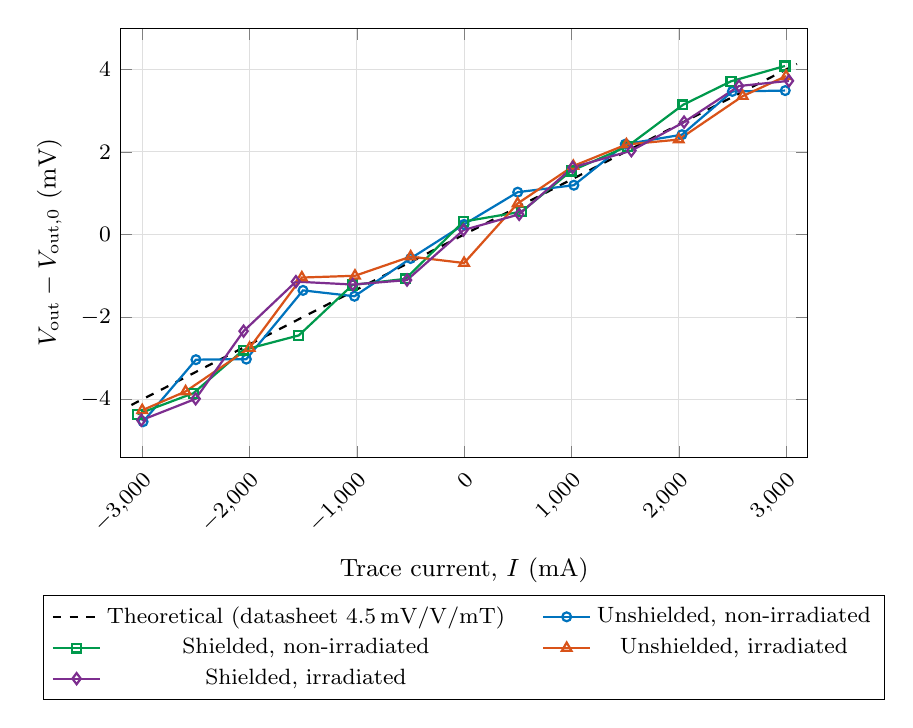
\begin{tikzpicture}
\begin{axis}[
    width=0.85\textwidth,
    height=0.58\textwidth,
    xlabel={Trace current, $I$ (mA)},
    ylabel={$V_{\text{out}} - V_{\text{out},0}$ (mV)},
    grid=major,
    grid style={gray!25},
    xmin=-3200, xmax=3200,
    axis lines=box,
    tick label style={font=\footnotesize},
    xticklabel style={rotate=45, anchor=north east},
    label style={font=\small},
    title style={font=\small},
    legend columns=2,
    legend style={
        at={(0.5,-0.32)},
        anchor=north,
        font=\footnotesize,
        draw=black,
        /tikz/every even column/.append style={column sep=0.4cm},
    },
]

% --- Theoretical expectation (slope = 1.332 mV/A = 0.001332 mV/mA) ---
\addplot[black, dashed, thick, domain=-3100:3100, samples=50] {0.001332*x};
\addlegendentry{Theoretical (datasheet \SI{4.5}{mV/V/mT})}

% --- Unshielded, non-irradiated (slope 1.315 mV/A, offset 12.603 mV removed) ---
\addplot[color={rgb,255:red,0;green,115;blue,189}, mark=o, mark size=1.6pt, thick]
    coordinates {
    (-2991.0,-4.534) (-2498.5,-3.032) (-2029.0,-3.019) (-1501.0,-1.354)
    (-1022.0,-1.496) (-499.0,-0.581) (-0.7,0.244) (499.0,1.025)
    (1022.0,1.193) (1501.0,2.187) (2029.0,2.417) (2498.5,3.465)
    (2991.0,3.485)
    };
\addlegendentry{Unshielded, non-irradiated}

% --- Shielded, non-irradiated (slope 1.447 mV/A, offset 12.393 mV removed) ---
\addplot[color={rgb,255:red,0;green,153;blue,76}, mark=square, mark size=1.6pt, thick]
    coordinates {
    (-3043.4,-4.354) (-2522.5,-3.844) (-2057.7,-2.799) (-1540.3,-2.444)
    (-1040.2,-1.223) (-546.2,-1.074) (-6.3,0.312) (535.4,0.553)
    (996.2,1.538) (1523.0,2.137) (2038.1,3.139) (2486.1,3.710)
    (2988.7,4.081)
    };
\addlegendentry{Shielded, non-irradiated}

% --- Unshielded, irradiated (slope 1.312 mV/A, offset 0.999 mV removed) ---
\addplot[color={rgb,255:red,217;green,83;blue,25}, mark=triangle, mark size=2pt, thick]
    coordinates {
    (-2999.0,-4.257) (-2595.0,-3.802) (-1999.0,-2.747) (-1512.0,-1.043)
    (-1017.0,-1.000) (-498.0,-0.536) (-0.7,-0.691) (498.0,0.750)
    (1017.0,1.658) (1512.0,2.179) (1999.0,2.299) (2595.0,3.351)
    (2999.0,3.835)
    };
\addlegendentry{Unshielded, irradiated}

% --- Shielded, irradiated (slope 1.342 mV/A, offset 1.211 mV removed) ---
\addplot[color={rgb,255:red,125;green,46;blue,143}, mark=diamond, mark size=2pt, thick]
    coordinates {
    (-3007.1,-4.498) (-2501.2,-3.980) (-2054.6,-2.341) (-1567.3,-1.142)
    (-1037.7,-1.212) (-532.1,-1.104) (-6.3,0.107) (512.5,0.488)
    (1011.4,1.626) (1557.8,2.030) (2048.6,2.722) (2560.6,3.596)
    (3025.4,3.721)
    };
\addlegendentry{Shielded, irradiated}

\end{axis}
\end{tikzpicture}
\caption{Current sweeps for the four test conditions with each sweep's fitted zero-current offset removed, so that only the gradient is compared, against the theoretical gradient (dashed). All measured sweeps lie close to the theoretical line.}
\label{fig:sensitivity-comparison}
\end{figure}

\subsection{Saturation Recovery and What It Means for a CubeSat}
\label{sec:disc-recovery}

Table~\ref{tab:recovery-summary} summarises the saturation recovery across all samples. The ceiling is within a few percent of $V_{\text{DD}}/3$ on every unit, confirming the bridge model of Section~\ref{sec:bridge-topology}, and it is symmetric about zero. Recovery takes 40 to $\SI{85}{\milli\second}$ depending on the unit, and on the three integrated boards the decay is a clean exponential with a time constant of 9 to $\SI{14}{\milli\second}$, with no difference between the non-irradiated and irradiated boards.

\begin{table}[H]
\centering
\caption{Summary of saturation recovery across all samples (means over both ceilings).}
\label{tab:recovery-summary}
\begin{tabular}{@{}lrrrr@{}}
\toprule
Group & Units & Ceiling (V) & Recovery (ms) & $\tau$ (ms) \\
\midrule
Sensor-only, non-irradiated (Samples 1--2) & 2 & 1.130 & 73.5 & --- \\
Sensor-only, irradiated (Samples 3--4) & 2 & 1.124 & 74.8 & --- \\
Integrated, non-irradiated (Board A) & 1 & 1.145 & 62.7 & 13.2 \\
Integrated, irradiated (Board B) & 1 & 1.148 & 65.0 & 13.3 \\
Integrated, fresh sensor (Board C) & 1 & 1.112 & 44.4 & 9.1 \\
\bottomrule
\end{tabular}
\end{table}

What this means depends on how often the on-board computer reads the magnetometer. Published CubeSat designs read magnetometers at rates from about \SI{1}{\hertz}, the rate of the whole attitude-control loop on InnoCube \cite{djebko_lelar}, up to about \SI{10}{\hertz} for a commercial CubeSat magnetometer \cite{nss_magnetometer}. At \SI{10}{\hertz} the sample interval is $T_s = \SI{100}{\milli\second}$, so the worst measured recovery time of $\SI{85}{\milli\second}$ (Sample 4) leaves a margin of only $\SI{15}{\milli\second}$. Comparing the recovery \emph{frequency} ($1/t_{\text{rec}} \approx 12$ to $\SI{25}{\hertz}$) with the sampling frequency is misleading, because a saturating event is not synchronised with the sampling clock. In the worst case the event ends just before a scheduled sample, and that sample is taken while the sensor is still recovering. An unrecovered reading would appear to a state estimator as a sudden impulse in the field and could trigger a false correction. The design quantity is therefore a guard window that covers the worst-case recovery with margin. Applying a conventional safety factor of 1.5 to 2 to the worst measured recovery gives a guard window of $\SI{127.5}{}$ to $\SI{170}{\milli\second}$:
\begin{equation}
T_{\text{guard}} = (1.5 \text{ to } 2) \times t_{\text{rec,max}} = (1.5 \text{ to } 2) \times \SI{85}{\milli\second} \approx \SI{127.5}{} \text{ to } \SI{170}{\milli\second}.
\end{equation}
This exceeds one sample interval at \SI{10}{\hertz}, so the first one or two readings after a saturating event should be discarded. At a \SI{1}{\hertz} loop the recovery is over long before the next sample and no blanking is needed. At sample rates of hundreds of hertz, such as the \SI{500}{\hertz} maximum configurable rate of one commercial magnetometer \cite{mm200_datasheet}, tens of consecutive samples would be affected, so a longer blanking period, or fusion with another attitude sensor during recovery, would be required.

Saturation is easy to detect in flight, because the output goes to a ceiling of about $\pm V_{\text{DD}}/3$ ($\pm\SI{1.1}{\volt}$), which is more than a thousand times larger than the output for Earth's field. Flight software can therefore recognise a saturating event from the reading itself and then apply the guard window. The sources of such events are off-nominal (Section~\ref{sec:strong-field-lit}): a normally operating magnetorquer of about $\SI{0.2}{\ampere\metre\squared}$ gives a few millitesla at a few centimetres \cite{isis_imtq}, which would shift the output by tens of millivolts but is well inside the CT100's $\pm\SI{50}{\milli\tesla}$ range. Saturation would instead come from a much closer or stronger source, such as a magnet near the sensor or magnetising equipment during ground handling. Stress-testing saturation is still worthwhile because it characterises the worst case the sensor must survive and recover from, regardless of which source causes it.

The recovery times measure how quickly the field was removed as much as how quickly the sensor responds. The datasheet bandwidth of $\SI{1}{\kilo\hertz}$ \cite{digikey_ct100} implies an electrical time constant of about $\SI{0.16}{\milli\second}$, far shorter than the 9 to $\SI{14}{\milli\second}$ fitted here. The magnet, by contrast, must travel a long way before its field is negligible. From Equation~\eqref{eq:disc-magnet}, the on-axis field of the LM-1618 falls to $\SI{50}{\milli\tesla}$, the edge of the CT100's operating range, about $\SI{15}{\milli\metre}$ from its face, but falls to $\SI{0.33}{\milli\tesla}$, the field that corresponds to the $\SI{5}{\milli\volt}$ settling band at $\SI{14.9}{\milli\volt\per\milli\tesla}$, only at about $\SI{110}{\milli\metre}$. Withdrawing the magnet over those $\SI{95}{\milli\metre}$ with a quick hand movement of roughly 1 to $\SI{2.5}{\metre\per\second}$ takes about 40 to $\SI{95}{\milli\second}$, which covers the whole measured range of 40 to $\SI{85}{\milli\second}$. The measured recovery is therefore consistent with the sensor simply following the falling field, and it should be read as an upper bound on the sensor's own recovery, which this method cannot resolve. The fitted time constant describes this combined process rather than a property of the sensor alone. This makes the guard window above conservative when a field is removed abruptly, for example when a magnetorquer is switched off. When a field is removed slowly, as when a magnetised object moves away, the output follows the field, and the end of the event is better detected by the output returning inside its linear range. These distances are indicative only, because the sensing axis lies in the plane of the package and the magnet was not withdrawn exactly along its own axis.

\todo{Planned measurement: repeat the saturation recovery five times on one integrated board in one session, with the same magnet and approach, and report the recovery time and time constant as mean $\pm$ standard deviation in Table~\ref{tab:recovery-summary}.}

\subsection{Offset Shift After Saturation}
\label{sec:disc-hysteresis}

The most significant finding of this work is that saturation moves the zero-field output without changing the gradient. On a fresh sensor with no magnetic history, two saturation events shifted the baseline by $\SI{16.1}{\milli\volt}$ (from $-4.8$ to $+\SI{11.3}{\milli\volt}$), while the gradient changed by only $-0.5\%$ and the response stayed linear (Section~\ref{sec:hysteresis}). Board A showed a similar shift of $+\SI{20.9}{\milli\volt}$ at the positive ceiling. At the sensor's sensitivity of about $\SI{14.9}{\milli\volt\per\milli\tesla}$ a shift of 16 to $\SI{21}{\milli\volt}$ is equivalent to a field of 1.1 to $\SI{1.4}{\milli\tesla}$, which is at least 15 times Earth's field of 25 to $\SI{65}{\micro\tesla}$ \cite{wmm}. This is consistent with the manufacturer's statement that a strong field can leave a stable, irreversible offset shift and that recalibration is recommended \cite{allegro_an133}, and it puts a size on the effect for this part. The datasheet offset specification of $\pm 5$~mV/V ($\pm\SI{16.6}{\milli\volt}$ at $V_{\text{DD}} = \SI{3.32}{\volt}$) \cite{ct100_datasheet} would still be met after the shift, so the part would not be flagged as out of specification even though the shift is large compared with the geomagnetic signal.

Because the gradient and linearity are unchanged, the shift behaves like a movement of the operating point, as expected if the free layer relaxes to a slightly different resting state after saturation. For a CubeSat this means that a one-point re-zeroing of the offset is sufficient after a saturating event, and that a full recalibration is not needed. The saturation can be detected from the reading itself (Section~\ref{sec:disc-recovery}), so the recommended procedure is to detect the ceiling, discard the guard window, and then re-estimate the offset before trusting the magnetometer again. In orbit the sensor is never in zero field, so the offset cannot simply be measured; it would instead be re-estimated by attitude-independent calibration against a geomagnetic field model, as demonstrated in flight for the MAGIC magnetometer on CINEMA \cite{archer2015}.

This also explains the difference in baseline between the non-irradiated and irradiated sweeps (about $+\SI{12}{\milli\volt}$ against about $+\SI{1}{\milli\volt}$). The non-irradiated board had been saturated before its sweeps, the irradiated board had not, and the fresh sensor shows that saturation alone moves the baseline by this amount. It is therefore not evidence of a radiation effect on the offset. One point remains open: Board B's own saturation events moved its baseline by only $\SI{1.6}{\milli\volt}$, so it is not yet known whether irradiated sensors respond to saturation differently. The evidence is also limited by the order of the events, because in every run the negative ceiling was reached before the positive one, so the direction of the field and the order of the events cannot yet be separated.

\subsection{Radiation Tolerance}
\label{sec:disc-radiation}

Ten sensors were exposed to an estimated $\SI{40.76}{\kilo rad}$(Si), and three were tested (two on sensor-only boards and one on the integrated board). No change was found in the saturation ceiling (0.5\% difference) or the recovery time (1.7\%), both smaller than the spread between non-irradiated units, in the recovery time constant (13.3 against $\SI{13.2}{\milli\second}$), or in the gradient, where the largest difference was 1.2 combined standard errors. This is what the literature predicts. Junction-level studies found no change at 5 and $\SI{10}{\mega rad}$(Si) \cite{tmr-bias-radiation,ren2012}, because the crystalline MgO barrier has far fewer trap sites for radiation-induced charge than the amorphous oxides in CMOS devices \cite{tid-basics-lanl}. The present result extends that evidence from bare junctions to a packaged, low-cost part tested in a circuit (Section~\ref{sec:lit-synthesis}), including, to the author's knowledge, the first saturation-recovery measurements after irradiation for such a part. The dose is modest by comparison with that work and with the $\SI{300}{\kilo rad}$(Si) used for a COTS magnetometer \cite{regoli2020}, but it is above the $\SI{10}{\kilo rad}$ component-level dose quoted for a commercial CubeSat magnetometer \cite{nss_magnetometer}. The test has clear limits. The dose is a calculated estimate with no dosimeter at the sensor. The sensors were unbiased and were not monitored during exposure, so transient effects that vanish afterwards were not seen; the bias-voltage study found no difference between biased and unbiased TMR sensors at a far higher dose \cite{tmr-bias-radiation}, which makes this less of a concern. X-rays test ionising dose only, not displacement damage or single-event effects. The comparison is between different units, with two sensor-only samples and one integrated board per group. The result is therefore evidence of no measurable permanent change in the tested sensors at this dose and under these conditions, not a qualification of the CT100 for flight.

\subsection{Magnetic Shielding}
\label{sec:disc-shielding}

Neither effect of the enclosure was resolved (Table~\ref{tab:hypothesis-outcomes}). The offset, which is where attenuation of the ambient field would appear, changed by 0.21 to $\SI{0.35}{\milli\volt}$, less than one ADC step. This is not evidence that the shield fails: Earth's field contributes at most about $\SI{1}{\milli\volt}$ along the sensing axis, so even a perfect shield could only have moved the offset by less than one ADC step on this readout. The gradient, which shows whether the ferrite disturbs the test field, changed by $+2.3\%$ on the irradiated board, within session-to-session variation, and by $+5$ to $+10\%$ on the non-irradiated board, where the larger value could reflect the ferrite slightly concentrating the trace field. The enclosure is also far from ideal: a closed shell of N95 ferrite would at best reduce an external field by a factor of about 200 (Section~\ref{sec:shielding-enclosure}), and the real enclosure has seams and a cable cut-out. A decisive test needs a stimulus larger than the readout resolution, such as a known field from a Helmholtz coil applied with and without the enclosure, with the change in offset measured on the DMM or a higher-resolution ADC; the shielding factor is then the ratio of the two offset changes. Mu-metal could then be tried if the ferrite proves insufficient. For flight, placing the magnetometer away from sources matters more than shielding the sensor \cite{nss_magnetometer}.

\subsection{Power Consumption}
\label{sec:disc-power}

Power is a first-order constraint on a CubeSat, so the cost of the sensing element is relevant. The datasheet gives a typical power consumption of $\SI{0.30}{\milli\watt}$ at $V_{\text{DD}} = \SI{3.0}{\volt}$ with a $\SI{30}{\kilo\ohm}$ bridge \cite{ct100_datasheet}. Since the bridge draws $V_{\text{DD}}/R$, where $R$ is the bridge resistance, this scales to about $\SI{0.36}{\milli\watt}$ at the $\SI{3.30}{\volt}$ used here, and to 0.27 to $\SI{0.54}{\milli\watt}$ over the 20 to $\SI{40}{\kilo\ohm}$ resistance range. It falls with the square of the supply voltage down to the datasheet minimum of $\SI{1.0}{\volt}$. For comparison, the AMR-based MAGIC instrument draws $\SI{0.5}{\watt}$ \cite{magic-radcube} and a commercial CubeSat magnetometer about $\SI{0.7}{\watt}$ \cite{nss_magnetometer}. These are complete instruments with electronics, so the comparison is not like for like, but it shows that the sensing element itself is a negligible part of a magnetometer's power budget; the power of a full instrument is set by the gain stage, ADC and processor. \todo{Planned measurement: connect the DMM in series with the supply to the standalone sensor board (DMM on its microamp or milliamp current range), record the supply current at zero field and with the sensor held at saturation, and report the current and the power $P = V_{\text{DD}} I$ here in place of the datasheet figure.}

\subsection{Limitations and Better Ways to Measure the Response}
\label{sec:disc-limitations}

The main weakness of the current method is the saturating stimulus. A hand-held magnet gives an uncontrolled withdrawal speed, an unknown field at the sensor, and poor repeatability, and its withdrawal takes about as long as the measured recovery (Section~\ref{sec:disc-recovery}), so the sensor's own recovery time could not be measured. A better method would use an electromagnet driven through a fast switch, so that the field is removed in a controlled, repeatable way, with the coil current and the sensor output recorded together on the oscilloscope and several repeats taken to give a mean and standard deviation. A linear actuator moving a magnet at a fixed speed would also work. The trace used for the current sweeps cannot saturate the sensor, because a field of about $\SI{20}{\milli\tesla}$ would need on the order of $\SI{180}{\ampere}$.

Other limitations are as follows.
\begin{itemize}
\item \textbf{Resolution.} With an unamplified 12-bit ADC, one step of $\SI{1.61}{\milli\volt}$ is about $\SI{108}{\micro\tesla}$ at the CT100's sensitivity, larger than Earth's field. The sensor itself is far quieter: its datasheet output noise of \SI{700}{\nano\volt\per\sqrt{\hertz}} at \SI{10}{\hertz} ($V_{\text{DD}} = \SI{1.0}{\volt}$) \cite{ct100_datasheet} corresponds to about \SI{0.16}{\micro\tesla\per\sqrt{\hertz}}, or roughly $\SI{0.5}{\micro\tesla}$ RMS over a \SI{10}{\hertz} bandwidth, about 1\% of Earth's field. The readout, not the sensor, therefore limits resolution in this work. A gain stage (whose slew rate would then have to be checked against the recovery measurement) or a higher-resolution ADC would be needed for geomagnetic sensing. \todo{Planned measurement: record \SI{60}{\second} of zero-field output with the DMM on its slowest, most precise setting, report the standard deviation, and convert it to a field with the \SI{14.9}{\milli\volt\per\milli\tesla} sensitivity.}
\item \textbf{Oscilloscope resolution.} At $\SI{500}{\milli\volt}$/div the oscilloscope steps are about $\SI{5}{\milli\volt}$, so the sensor-only baselines are not interpretable and the ceilings carry about $\pm\SI{5}{\milli\volt}$ of uncertainty.
\item \textbf{Sample size and design.} There are two sensor-only samples per group, one board per group on the integrated board, a single dose level, and the irradiated and non-irradiated comparison is across different units.
\item \textbf{Hysteresis test.} The two sensors tested were saturated negative first, and only one fresh sensor was tested in a controlled before-and-after sequence.
\item \textbf{Field model.} The predicted gradient carries a $-5\%$ to $+7\%$ uncertainty from the tolerance on the sensor's height inside its package and the package stand-off, and the Ansys model still needs to be evaluated at the datasheet sensor height (Section~\ref{sec:field-validation}).
\item \textbf{Scope of the project.} Temperature effects were studied separately by the project partner and are not covered here.
\end{itemize}




\section{Conclusions and Future Work}
\label{sec:conclusions}

\textbf{Conclusions.} This project characterised a low-cost commercial TMR sensor, the CT100, using two purpose-built PCBs, a field model built from the board stack-up and the datasheet sensor position, and instruments that were validated against each other. For the conditions tested, the research question of Section~\ref{sec:research-question} is answered as follows.
\begin{itemize}
\item \textbf{Bridge behaviour.} The saturation ceiling is within about 5\% of $\pm V_{\text{DD}}/3$ on every unit tested and symmetric about zero, as derived from the bridge topology (H1 supported).
\item \textbf{Sensitivity.} The measured current-to-output gradient agrees with the field model within $-5\%$ to $+9\%$, with the mean within 1\%, equivalent to 4.3 to $\SI{4.9}{\milli\volt\per\volt\per\milli\tesla}$ against a typical datasheet value of 4.5. The response is linear, with $R^2$ of 0.97 or higher (H2 supported).
\item \textbf{Recovery.} After saturation the output settles within $\SI{5}{\milli\volt}$ of its baseline in 40 to $\SI{85}{\milli\second}$. This is about the time a hand-withdrawn magnet takes to fall below the settling field, so it is an upper bound on the sensor's own recovery. On that bound, a $\SI{10}{\hertz}$ magnetometer should discard the first one or two samples after a saturating event, and at $\SI{1}{\hertz}$ no action is needed (H3 partly supported).
\item \textbf{Lasting effect of saturation.} Saturation shifts the zero-field offset by about 13 to $\SI{21}{\milli\volt}$ (1 to $\SI{1.4}{\milli\tesla}$ equivalent) without changing the gradient or the linearity, so the offset must be re-estimated after a saturating event (H4 rejected). This matches the manufacturer's note on offset shift and puts a size on it for the CT100.
\item \textbf{Radiation.} No measurable permanent change was found in ceiling, recovery, time constant or gradient after an estimated $\SI{40.76}{\kilo rad}$(Si) of unbiased X-ray exposure, as expected from junction-level studies (H5 supported for the three units tested). This is evidence for the tested units and dose, not a flight qualification.
\item \textbf{Shielding.} The ferrite enclosure changed the offset by less than one ADC step, as expected when the ambient field contributes at most about $\SI{1}{\milli\volt}$, and did not clearly disturb the test field. Its effectiveness against external fields remains unmeasured and needs a known applied field (H6 unresolved and partly supported).
\item \textbf{Power and resolution.} The bridge consumes about 0.3 to $\SI{0.5}{\milli\watt}$, a negligible part of a magnetometer power budget. The sensor's intrinsic noise of about $\SI{0.16}{\micro\tesla\per\sqrt{\hertz}}$ would resolve Earth's field, but the unamplified 12-bit readout used here could not.
\end{itemize}

\textbf{Significance.} The CT100 is a promising low-cost COTS candidate for CubeSat magnetometry. It showed no measurable permanent change after the dose tested, survives saturation, settles within at most tens of milliseconds and keeps its gradient. Its one lasting change, a shift in its zero point, can be detected from the reading itself and corrected by the kind of in-flight offset calibration already used for chip-scale magnetometers \cite{archer2015}. The work also provides a reusable, low-cost test method, from a PCB trace field source modelled from the stack-up to microcontroller logging validated against a DMM, that can be applied to other COTS TMR parts. More units, more dose levels and a readout with sufficient resolution are needed before flight use.

\textbf{Future work.}
\begin{itemize}
\item Replace the hand-held magnet with a controlled, repeatable saturation source (an electromagnet with a fast switch) and record several repeats per sample.
\item Repeat the hysteresis test on several fresh sensors, with the positive ceiling first as well as the negative, and on a fresh irradiated sensor, and implement and test a firmware procedure that detects the ceiling, applies the guard window and re-estimates the offset.
\item Monitor sensors during irradiation, state the bias condition, and extend the tests to more dose levels and to proton irradiation.
\item Test shielding with a known external field and a higher-resolution measurement, and try mu-metal.
\item Add a gain stage or a higher-resolution ADC and measure the noise floor in field units.
\item Re-run the Ansys model at the datasheet sensor height, and combine these results with the thermal-cycling results of the project partner.
\end{itemize}

\clearpage

\section*{Acknowledgements}
\addcontentsline{toc}{section}{Acknowledgements}

The author thanks project supervisor Dariusz Kacprzak for guidance throughout this project, and project partner Daniel Tieu for his work on the parallel thermal-cycling test campaign. \todo{Add any further acknowledgements -- e.g.\ workshop/lab staff, the radiation-testing facility or operator, or funding sources -- once confirmed.}

% Nitish, Aaron, Arnesh, Alex, jensen, Uzayr

% fix formatting number an TOC

\clearpage


\begin{thebibliography}{99}
\sloppy

\bibitem{survey-magnetic-sensing}
``A survey on magnetic sensing and communication: Technologies, sensors, and applications,'' \emph{IEEE} journal article, IEEE Xplore. \todo{Add authors, journal name, volume and year from your copy.}

\bibitem{bennett2021}
J.\ S.\ Bennett, B.\ E.\ Vyhnalek, H.\ Greenall, E.\ M.\ Bridge, F.\ Gotardo, S.\ Forstner, G.\ I.\ Harris, F.\ A.\ Miranda, and W.\ P.\ Bowen, ``Precision magnetometers for aerospace applications: A review,'' \emph{Sensors}, vol.~21, no.~16, art.~5568, 2021, doi: 10.3390/s21165568.

\bibitem{amr-gmr-hall-bridging}
``Bridging the gap between AMR, GMR, and Hall magnetic sensors,'' IEEE conference paper, IEEE Xplore. \todo{Add authors, conference name and year from your copy.}

\bibitem{magic-radcube}
J.\ P.\ Eastwood \emph{et al.}, ``In flight performance of the MAGIC magnetoresistive magnetometer on the RadCube CubeSat,'' \emph{Space Science Reviews}, vol.~221, art.~45, 2025, doi: 10.1007/s11214-025-01170-w.

\bibitem{julliere1975}
M.\ Julli\`ere, ``Tunneling between ferromagnetic films,'' \emph{Physics Letters A}, vol.~54, no.~3, pp.~225--226, 1975.

\bibitem{parkin2004}
S.\ S.\ P.\ Parkin \emph{et al.}, ``Giant tunnelling magnetoresistance at room temperature with MgO (100) tunnel barriers,'' \emph{Nature Materials}, vol.~3, pp.~862--867, 2004.

\bibitem{yuasa2004}
S.\ Yuasa, T.\ Nagahama, A.\ Fukushima, Y.\ Suzuki, and K.\ Ando, ``Giant room-temperature magnetoresistance in single-crystal Fe/MgO/Fe magnetic tunnel junctions,'' \emph{Nature Materials}, vol.~3, pp.~868--871, 2004.

\bibitem{alves-thesis}
P.\ F.\ L.\ Alves, ``Radiation hardness assessment of MR sensors for space applications,'' M.Sc.\ thesis, Instituto Superior T\'ecnico, Lisbon. [Online]. Available: \url{https://www.lip.pt/~space/Teses/MsC_Thesis_PedroAlves.pdf}

\bibitem{wisniowski2021}
P.\ Wi\'sniowski, M.\ Nawrocki, J.\ Wrona, S.\ Cardoso, and P.\ P.\ Freitas, ``Bias voltage dependence of sensing characteristics in tunneling magnetoresistance sensors,'' \emph{Sensors}, vol.~21, 2021. [Online]. Available: \url{https://www.ncbi.nlm.nih.gov/pmc/articles/PMC8038319/}

\bibitem{archer2015}
M.\ O.\ Archer \emph{et al.}, ``The MAGIC of CINEMA: first in-flight science results from a miniaturised anisotropic magnetoresistive magnetometer,'' \emph{Annales Geophysicae}, vol.~33, pp.~725--735, 2015, doi: 10.5194/angeo-33-725-2015.

\bibitem{tmr-bias-radiation}
``Radiation tolerance of tunneling magnetoresistance sensors under bias voltage,'' \emph{Science China Physics, Mechanics \& Astronomy}, 2025. [Online]. Available: \url{https://link.springer.com/article/10.1007/s11433-025-2784-y} \todo{Add the author list from the article page.}

\bibitem{nguyen2010}
H.\ Nguyen, A.\ Persson, and G.\ Thornell, ``Material- and fabrication-governed performance of a tunnelling magnetometer,'' 2010. [Online]. Available: \url{https://ans.vast.vn/index.php/oms/article/view/62/63} (accessed Oct.\ 2026).

\bibitem{ren2012}
F.\ Ren, A.\ Jander, P.\ Dhagat, and C.\ Nordman, ``Radiation tolerance of magnetic tunnel junctions with MgO tunnel barriers,'' \emph{IEEE Transactions on Nuclear Science}, vol.~59, no.~6, pp.~3034--3038, 2012.

\bibitem{seifu2023}
D.\ Seifu, Q.\ Peng, K.\ Sze, J.\ Hou, F.\ Gao, and Y.\ Lan, ``Electromagnetic radiation effects on MgO-based magnetic tunnel junctions: A review,'' 2023. [Online]. Available: \url{https://www.ncbi.nlm.nih.gov/pmc/articles/PMC10223111/}

\bibitem{tid-basics-lanl}
``Basic Mechanisms: Total Ionizing Dose,'' Los Alamos National Laboratory presentation.

\bibitem{regoli2020}
L.\ H.\ Regoli, M.\ B.\ Moldwin, C.\ Raines, T.\ A.\ Nordheim, C.\ A.\ Miller, M.\ Carts, and S.\ A.\ Pozzi, ``Radiation tolerance of the PNI RM3100 magnetometer for a Europa lander mission,'' \emph{Geoscientific Instrumentation, Methods and Data Systems}, vol.~9, pp.~499--507, 2020, doi: 10.5194/gi-9-499-2020.

\bibitem{nss_magnetometer}
NewSpace Systems, ``NSS Magnetometer,'' data sheet. [Online]. Available: \url{https://www.cubesatshop.com/wp-content/uploads/2016/06/NSS-Magnetometer-1.pdf} (accessed Oct.\ 2026).

\bibitem{isis_imtq}
Innovative Solutions In Space (ISISpace), ``iMTQ magnetorquer board,'' product brochure.

\bibitem{openstax_up2}
S.\ J.\ Ling, J.\ Sanny, and W.\ Moebs, \emph{University Physics Volume 2}. Houston, TX, USA: OpenStax, 2016, Sections 12.2 and 12.4. [Online]. Available: \url{https://openstax.org/books/university-physics-volume-2/pages/12-2-magnetic-field-due-to-a-thin-straight-wire}

\bibitem{wmm}
NOAA National Centers for Environmental Information, ``World Magnetic Model.'' [Online]. Available: \url{https://www.ncei.noaa.gov/products/world-magnetic-model} (accessed Oct.\ 2026).

\bibitem{ct100_datasheet}
Allegro MicroSystems, ``CT100 1D linear sensor,'' data sheet CT100-DS, Rev.~8, Sept.~2026. [Online]. Available: \url{https://www.allegromicro.com/-/media/files/datasheets/ct100-datasheet.pdf}

\bibitem{allegro_an133}
Allegro MicroSystems, ``AN133: What is XtremeSense TMR?'' application note. [Online]. Available: \url{https://www.allegromicro.com/-/media/files/application-notes/an133-what-is-xtremesense-tmr.pdf} (accessed Oct.\ 2026).

\bibitem{digikey_ct100}
DigiKey, ``CT100LW-FS6 product listing (Allegro MicroSystems).'' [Online]. Available: \url{https://www.digikey.com/en/products/detail/allegro-microsystems/CT100LW-FS6/22114166} (accessed Oct.\ 2026).

\bibitem{lm1618_datasheet}
Jaycar Electronics, ``Rare earth magnets: LM-1618, LM-1620 and LM-1622,'' data sheet. [Online]. Available: \url{https://media.jaycar.com.au/product/images/LM1618_datasheetMain_76111.pdf} (accessed Oct.\ 2026).

\bibitem{camacho2013}
J.\ M.\ Camacho and V.\ Sosa, ``Alternative method to calculate the magnetic field of permanent magnets with azimuthal symmetry,'' \emph{Revista Mexicana de F\'isica E}, vol.~59, pp.~8--17, 2013. [Online]. Available: \url{https://www.redalyc.org/pdf/570/57048158002.pdf}

\bibitem{shulman2022}
D.\ Shulman, ``Magnetic field of a permanent magnet,'' arXiv:2207.09911, 2022. [Online]. Available: \url{https://arxiv.org/abs/2207.09911}

\bibitem{stm32g4_rm}
STMicroelectronics, ``RM0440: STM32G4 Series advanced Arm-based 32-bit MCUs,'' reference manual.

\bibitem{ina219_datasheet}
Texas Instruments, ``INA219 zero-drift, bidirectional current/power monitor with I2C interface,'' data sheet.

\bibitem{poivey_rha}
C.\ Poivey, ``Radiation hardness assurance for space systems,'' IEEE Nuclear and Space Radiation Effects Conference (NSREC) Short Course, 2002.

\bibitem{escc22900}
European Space Components Coordination, ``Total dose steady-state irradiation test method,'' ESCC Basic Specification No.~22900, Issue~3, Mar.~2007. [Online]. Available: \url{https://escies.org/download/specdraftapppub?id=1240}

\bibitem{sangal2023}
M.\ Sangal, M.\ Anikeeva, S.\ C.\ Priese, H.\ Mattern, J.-B.\ H\"ovener, and O.\ Speck, ``MR based magnetic susceptibility measurements of 3D printing materials at 3 Tesla,'' \emph{Journal of Magnetic Resonance Open}, vol.~16--17, art.~100138, 2023, doi: 10.1016/j.jmro.2023.100138. [Online]. Available: \url{https://pub.dzne.de/record/266487/files/DZNE-2023-01172.pdf}

\bibitem{fitzpatrick_shielding}
R.\ Fitzpatrick, ``Magnetic shielding,'' in \emph{Classical Electromagnetism} (lecture notes), University of Texas at Austin. [Online]. Available: \url{https://farside.ph.utexas.edu/teaching/jk1/lectures/node63.html}

\bibitem{msc_mumetal}
Magnetic Shield Corporation, ``MuMETAL\textsuperscript{\textregistered} fully annealed foil,'' data sheet. [Online]. Available: \url{https://www.magnetic-shield.com/content/MuMetal%20Fully%20Annealed%20Foil%20Data.pdf} (accessed Oct.\ 2026).

\bibitem{tdk_n95}
TDK Electronics (EPCOS), ``SIFERRIT material N95,'' ferrite material data sheet. [Online]. Available: \url{https://www.tdk-electronics.tdk.com} (accessed Oct.\ 2026).

\bibitem{yunlu_nanocrystalline}
Qingdao Yunlu Energy Technology Co., Ltd., ``Nanocrystalline: soft magnetic material,'' product page. [Online]. Available: \url{https://ylenergytech.com/5-3-nanocrystalline/200915/} (accessed Oct.\ 2026).

\bibitem{djebko_lelar}
K.\ Djebko, T.\ Baumann, E.\ Dilger, F.\ Puppe, and S.\ Montenegro, ``LeLaR: The first in-orbit demonstration of an AI-based satellite attitude controller,'' arXiv:2512.19576, 2025.

\bibitem{mm200_datasheet}
AAC Clyde Space, ``MM200 magnetometer,'' data sheet. [Online]. Available: \url{https://www.aac-clyde.space/wp-content/uploads/2021/11/MM200.pdf} (accessed Oct.\ 2026).

\end{thebibliography}

\end{document}